\documentclass[a4paper, 11pt, oneside, polutonikogreek, french]{article}
\usepackage[T1]{fontenc}
\usepackage{aurical}
\usepackage{pdflscape}
% Babel package:
\usepackage[french]{babel}
% Load encoding definitions (after font package)
\usepackage{textalpha}
\usepackage{listings}
\usepackage{bbding}
\lstset{basicstyle=\ttfamily}

\usepackage[dvipsnames]{xcolor}
\usepackage{eso-pic,graphicx}
\usepackage[top=50mm, bottom=50mm, outer=29mm, inner=29mm]{geometry}
\setlength{\columnsep}{90pt}

% With XeTeX$\$LuaTeX, load fontspec after babel to use Unicode
% fonts for Latin script and LGR for Greek:
\ifdefined\luatexversion \usepackage{fontspec}\fi
\ifdefined\XeTeXrevision \usepackage{fontspec}\fi

% "Lipsiakos" italic font `cbleipzig`:
\newcommand*{\lishape}{\fontencoding{LGR}\fontfamily{cmr}%
		       \fontshape{li}\selectfont}
\DeclareTextFontCommand{\textli}{\lishape}

\usepackage{sectsty}
\usepackage[titles]{tocloft}

\allsectionsfont{\Fontauri}
\sectionfont{\Fontauri\Huge}
\subsectionfont{\Fontauri\LARGE}
\subsubsectionfont{\Fontauri\Large}

\usepackage{setspace}
\onehalfspacing

\usepackage{booktabs}
\usepackage{graphicx}
\setlength{\emergencystretch}{15pt}
\graphicspath{ {./figures/} }
\usepackage[figurename=]{caption}
\usepackage{float}
\usepackage{fancyhdr}
\usepackage{microtype}
\usepackage{tocloft}
\cftsetindents{section}{1em}{3em}

% change color of text, example replace all \color{Goldenrod} with \color{lightgray}

\makeatletter % change only the display of \thepage, but not \thepage itself:
\patchcmd{\ps@plain}{\thepage}{\bfseries\large\color{White}{\thepage}}{}{}
\makeatother

\color{White}

\begin{document}
\Fontauri
\renewcommand{\cftfigfont}{\Fontauri}
\renewcommand{\cftfigpagefont}{\Fontauri}

\renewcommand{\cftsecfont}{\Fontauri}
\renewcommand{\cftsubsecfont}{\Fontauri}
\renewcommand{\cftsubsubsecfont}{\Fontauri}
% fix toc page numbers
\let\origcftsecfont\cft
\let\origcftsecpagefont\cftsecpagefont
\let\origcftsecafterpnum\cftsecafterpnum
\renewcommand{\cftsecpagefont}{\Fontauri{\origcftsecpagefont}}
\renewcommand{\cftsecafterpnum}{\Fontauri{\origcftsecafterpnum}}
\let\origcftsubsecpagefont\cftsubsecpagefont
\let\origcftsubsecafterpnum\cftsubsecafterpnum
\renewcommand{\cftsubsecpagefont}{\Fontauri{\origcftsubsecpagefont}}
\renewcommand{\cftsubsecafterpnum}{\Fontauri{\origcftsubsecafterpnum}}
\let\origcftsubsubsecpagefont\cftsubsubsecpagefont
\let\origcftsubsubsecafterpnum\cftsubsubsecafterpnum
\renewcommand{\cftsubsubsecpagefont}{\Fontauri{\origcftsubsubsecpagefont}}
\renewcommand{\cftsubsubsecafterpnum}{\Fontauri{\origcftsubsubsecafterpnum}}

\renewcommand{\thefigure}{\Fontauri{\arabic{figure}}}
\renewcommand\thefootnote{\Fontauri{\arabic{footnote}}}
\let\oldfootnote\footnote
    \renewcommand{\footnote}[1]{\oldfootnote{\Fontauri\large#1}}

\AddToShipoutPictureBG{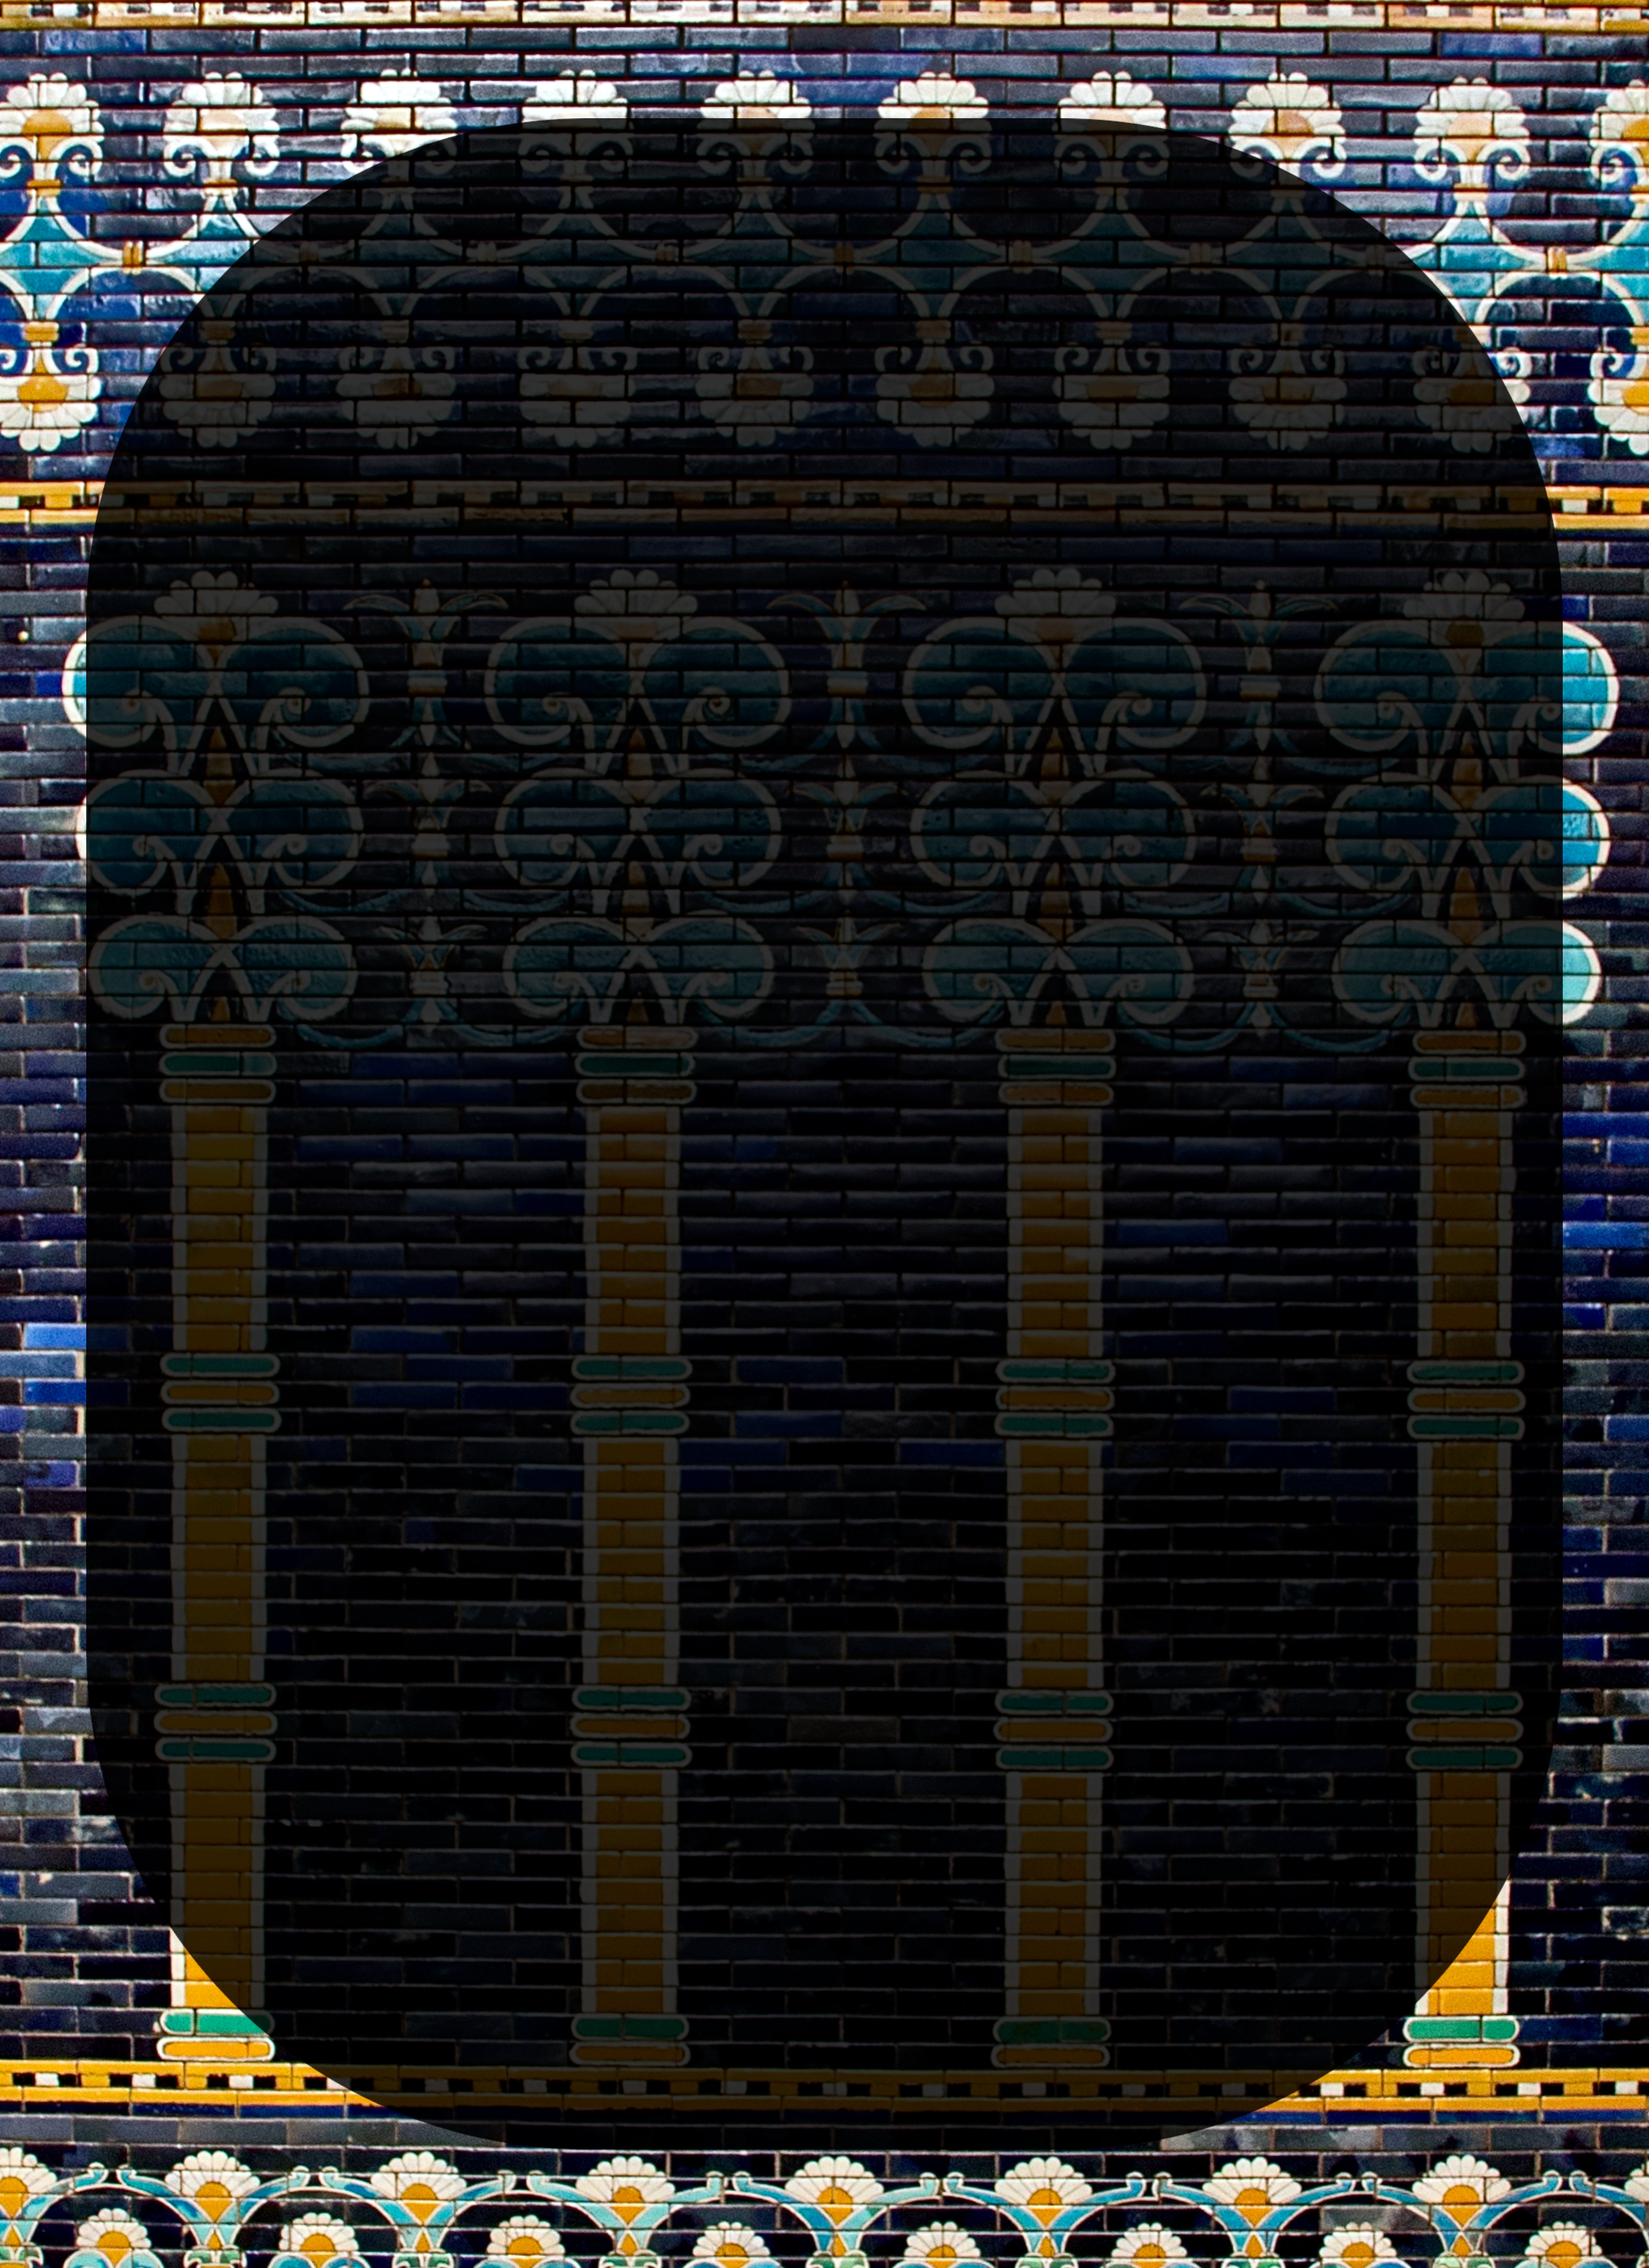
\includegraphics[width=\paperwidth,height=\paperheight]{ishtargate.jpeg}}

\begin{titlepage} % Suppresses headers and footers on the title page
	\centering % Centre everything on the title page
	%\scshape % Use small caps for all text on the title page

	%------------------------------------------------
	%	Title
	%------------------------------------------------
	
	\rule{\textwidth}{1.6pt}\vspace*{-\baselineskip}\vspace*{2pt} % Thick horizontal rule
	\rule{\textwidth}{0.4pt} % Thin horizontal rule
	
	\vspace{1\baselineskip} % Whitespace above the title
	
	{\scshape\Huge La Fin de Babylone}
	
	\vspace{1\baselineskip} % Whitespace above the title

	\rule{\textwidth}{0.4pt}\vspace*{-\baselineskip}\vspace{3.2pt} % Thin horizontal rule
	\rule{\textwidth}{1.6pt} % Thick horizontal rule
	
	\vspace{1\baselineskip} % Whitespace after the title block
	
	%------------------------------------------------
	%	Subtitle
	%------------------------------------------------
	
	{\scshape Par \Large Guillaume Apollinaire} % Subtitle or further description
	
	\vspace*{1\baselineskip} % Whitespace under the subtitle
	
        {\scshape Ouvrage orné de seize illustrations hors texte. \\\small D'après Rubens, Le Dominiquin, Aldegraver, Nicolas Poussin, Antoine Coypel, Eugène Delacroix, Rochegrosse, etc.} % Subtitle or further description
    
	%------------------------------------------------
	%	Editor(s)
	%------------------------------------------------
        \vspace*{\fill}

	\vspace{1\baselineskip}

	{\small\scshape Paris, 1922. Première Édition, 1914.}
	
	{\small\scshape{Bibliothèque des Curieux.\\ 4, Rue de Furstenberg, 4.}}
	
	\vspace{0.5\baselineskip} % Whitespace after the title block

        \scshape Internet Archive Online Edition  % Publication year
	
	{\scshape\small Utilisation non commerciale --- Partage dans les mêmes conditions 4.0 International} % Publisher
\end{titlepage}
\pagestyle{fancy}
\fancyhf{}
\cfoot{\Fontauri{\thepage}}
\Large
\setlength{\parskip}{1mm plus1mm minus1mm}
\clearpage
\tableofcontents
\clearpage
\begin{landscape}
\begin{figure}[H]
\centering
\includegraphics[height=0.91\textheight,keepaspectratio]{plates/Mort_de_Sardanapale_-_Eugène_Delacroix_-_Musée_du_Louvre_Peintures_RF_2346.jpg}
\caption{\Fontauri Pl. 1. --- La Mort de Sardanapale. \emph{Eug. Delacroix.}}
\end{figure}
\end{landscape}
\clearpage
\section{Chapitre Premier. --- Le Départ de Lutèce.}
\begin{center}
\scshape
\small
Les fredaines de Vietrix. --- Un grand industriel gaulois. --- La polychromie. --- Les distractions de Lutèce. --- Petites orgies spéculatives. --- Les caravanes de Phéniciens. --- Les premières invasions celtes. --- Caractère des Parisiens. --- Une fille d'Érin. --- A travers la Gaule. --- Sous un dolmen. --- Le druide. --- Leur culte. --- L'oracle de la croix gammée.
\end{center}
\paragraph{}
Ce fut sans enthousiasme que le jeune Vietrix, au moment où se préparaient les fêtes du Printemps, quitta l'île de Lutèce. Il aimait ce paysage dans lequel il était né, le fleuve sinueux, ses rives couvertes de roseaux, et dans le lointain, au nord et au sud, les deux collines verdoyantes. Il aimait la capitale du pays des Parisiens et ses plaisirs. Mais la volonté paternelle était formelle. Il comprenait lui-même que ses nombreuses fredaines l'obligeaient à une retraite momentanée.

Son père était l'un des industriels les plus riches et considérés de cette partie de la Gaule. Sous sa direction, d'habiles ouvriers apprenaient à travailler artistement le bronze, l'étain, le fer et l'or. De l'Armorique à la Savoie, les pommeaux d'épée et les boucles de ceinturon provenant de la maison Vietrix étaient fort appréciés. Les marchands des régions de l'est où campaient les tribus celtes et des montagnes du sud où avaient pris refuge les Ibères faisaient de nombreux achats chez lui. Et quant aux élégantes de l'île et des environs, elles savaient où trouver les plus élégants bijoux, colliers, pendentifs ou bracelets.

Un art nouveau, celui de la polychromie, venait de faire son apparition dans les Gaules. L'incrustation dans les alliages au bronze présentait un aspect plaisant et dont tous les riches personnages raffolaient déjà. Le travail se faisait principalement au corail rouge.

C'était là le prétexte que le père Vietrix avait trouvé pour éloigner des plaisirs de Lutèce son rejeton, dont la présence n'était d'ailleurs nullement nécessaire à la marche des affaires. Le jeune homme, en effet, ne se sentait pas de goût pour la surveillance des ateliers de la maison paternelle. Certes il appréciait la rare qualité de l'art parisien. Pour lui-même et ses maîtresses il prisait fort les bijoux riches et légers. Mais sa tendance naturelle était à un dilettantisme général. Un travail mécanique et régulier le rebutait. Il se laissait aller à rêver de destinées étranges et fabuleuses. Il appartenait déjà à la génération qui dépense plutôt qu'à celle qui amasse.

Il savait à l'occasion manier les armes, combattre un ennemi corps à corps ou réduire les animaux à la chasse. Il était fort, grand, bien découplé, les cheveux châtains et les yeux clairs. Récemment encore, dans les plaines qui s'étendent au-delà de la colline du nord, il avait détruit, en compagnie de quelques amis, un gros troupeau de ruminants à bosses. Mais il se plaisait surtout aux controverses d'art, de philosophie et de littérature, pour lesquelles il ne trouvait malheureusement pas beaucoup de partenaires. La lutte pour la vie était âpre, les ambitions nombreuses, rares étaient ceux auxquels leurs occupations permettaient de telles distractions. L'esprit public était cependant à Lutèce des mieux cultivés.

Vietrix, féru de discussions, ne manquait point d'inviter tous les notoires étrangers de passage à des repas où les plus graves sujets étaient agités. Ces petites fêtes spéculatives, à la vérité, se terminaient généralement dans l'orgie, Vietrix étant accoutumé de convier à ses agapes un certain nombre de jeunes personnes qui s'efforçaient de faire dévier la conversation et y réussissaient fort bien.

\bigskip
\centerline{\EightStarTaper}
\centerline{\EightStarTaper\EightStarTaper}
\bigskip

Vietrix avait donc dû quitter tous ses bons amis parisiens, sa bande, pour se rendre d'ordre paternel aux Iles d'Hyères, où des pêcheurs récoltaient, disait-on, le corail en grande quantité. Précisément un nombreux cortège de Phéniciens, avec lesquels la maison Vietrix père était depuis longtemps en relations commerciales, venait de passer à Lutèce. Ces hommes bruns arrivaient des pays de Cornouailles où sont les grandes mines d'étain. Leurs navires chargés, ils avaient décidé de regagner à travers les Gaules les rivages de la Méditerranée. En route, chez les Ligures et les Celtes, qui commençaient de déborder vers le Rhin, ils auraient toujours l'occasion de conclure quelque affaire.

Dans le pays, de grands garçons aux corps très blancs, aux larges cheveux blonds, aux yeux bleus rôdaient depuis quelque temps. Ils appartenaient aux tribus des Celtes dont la marche en avant était déjà signalée vers l'est. Ces jeunes gens étaient fort instruits, versés dans la poésie religieuse et profane. Ils cultivaient notamment la satire composant de petits morceaux agressifs que les guerriers devaient réciter à leurs adversaires avant que de se précipiter sur eux la lance en avant. Vietrix, comme il est juste, s'était tout de suite lié avec eux, et cela avait mécontenté les anciens de la tribu, qui accusaient ces Celtes de préparer en sous-main l'invasion de leurs hordes.

Il n'était pas, lui, de race proprement ligure. Déjà tant de populations s'étaient succédé sur les rives de la Seine ! Car si Lutèce était, à la vérité, entourée d'affreux marécages, la situation générale n'en était pas moins sûre au point de vue militaire et avantageuse au point de vue commercial. Les Parisiens formaient déjà un petit groupe spécial, réputé pour ses habiles artisans, ses goûts artistiques et un certain esprit désabusé.

Vietrix avait donc embrassé sa maîtresse, une fillette d'Erin aux longs cheveux roux et aux yeux couleur de mer, fillette tombée dans cette ville on ne sait par quel hasard. Il l'aimait sans doute un peu, il l'aimait parce qu'il avait le premier dompté sa petite âme farouche et plié son corps, ce joli corps d'une blancheur éblouissante, à de savantes voluptés. Mais l'amour est caprice ! Vietrix baisa donc la bouche écarlate de l'enfant qui dormait, la pointe de ses seins menus, s'en fut dire adieu à quelques-uns de ses amis. Puis il prit rang dans la troupe des Phéniciens.

Il emportait un léger bagage, des armes et quelques tuniques de chanvre. Il avait eu soin principalement de se munir à la maison paternelle d'un sac gonflé de poudre d'or. Cette monnaie fut toujours considérée en tous pays comme de première qualité.

\bigskip
\centerline{\EightStarTaper}
\centerline{\EightStarTaper\EightStarTaper}
\bigskip

La route fut pénible. Le cortège suivait de préférence le cours des rivières. Mais une nuit, assaillis par l'orage, les voyageurs se perdirent dans la forêt. Enfin un grand dolmen auprès duquel était construit une bâtisse ronde et basse leur offrit un abri. C'étaient là des monuments funéraires. Le cadavre d'un chef y avait récemment reçu les honneurs. Ils s'installèrent tant bien que mal.

Vietrix dormit cette nuit-là d'un sommeil agité. Des regrets l'assaillirent. Il revoyait la tranquillité de la ville natale, il distinguait l'imprudence de son équipée. Que ce repos, parmi les cadavres, était donc dépourvu de confort ! Ni lui ni ses amis n'avaient osé toucher aux vivres que des mains pieuses avaient disposés à l'usage des morts. Ah ! s'il avait jamais eu l'intention de pousser son voyage au-delà des Iles d'Hyères, il déplorait maintenant son égarement !

Le lendemain matin, la petite troupe, à peine éveillée, vit arriver un homme vêtu d'une longue robe blanche. Il portait à la main une serpe d'or. Vietrix avait déjà entendu dire que dans certaines forêts des rites nouveaux, venus des îles du Nord, s'étaient établis. Sa petite maîtresse lui avait certains soirs raconté de mystérieuses légendes. Sans doute cet homme étrange procédait-il d'un tel culte.

C'était un Druide, en effet. Vietrix fut enchanté de faire sa connaissance. Le prêtre, qui paraissait être chez lui, offrit à tous les souhaits de l'hospitalité. Le Parisien s'étonna de tant de libéralisme, car il savait que les cérémonies funéraires et le culte des pierres remontaient à la plus antique tradition gauloise.

Le Druide, cependant, lui en donna l'explication. Lui aussi reconnaissait les Divinités essentielles du Feu, des Sources et des Bois. Qui donc des humains, depuis les temps les plus reculés, eût négligé d'adorer ces forces de la nature, gracieuses et bienfaisantes ? C'était là l'héritage de tous. Du reste le prêtre estimait qu'il n'avait point le droit de répudier les divinités des pays nouveaux où son culte pénétrait peu à peu. Il acceptait même les sacrifices humains aux divinités redoutables de la guerre et de l'amour. Il convenait en son métier d'être opportuniste.

Vietrix, que les différents problèmes de la vie avaient toujours intéressé, fut enchanté de s'entretenir avec cet homme érudit et éminent. Et en fin de compte il lui confia la singulière neurasthénie dont il souffrait. Plus rien ne le satisfaisait. Quoiqu'il connût Lutèce dans les recoins, il avait quitté la ville avec regret, il ne savait s'il devait arrêter là son voyage, ou bien poursuivre son aventure.

Le prêtre réfléchit longuement. Puis ayant regardé Vietrix dans les yeux, il lui parla ainsi :

--- Mon fils, ton destin n'est pas ici. Tes tourments ne sauraient trouver pour l'heure, parmi les peuples rudes que nous sommes, une satisfaction. Plus tard tu reviendras à nous, sage et expérimenté.

C'est une femme qui doit te sauver. Cette femme, je ne sais qui elle est. Je vois cependant qu'elle est née sous le signe sacré que du bout de ma serpe je trace sur le rocher. Vois. A cet indice tu la reconnaîtras.

--- Et dans quelles régions, mon père ?

--- Là-bas, vers les terres chaudes, vers le pays où chaque jour le soleil fait son apparition.

--- Je n'arrêterai point ma marche avant que de l'avoir rencontrée ?

--- Tu ne connaîtras point le repos avant.

Ce disant le druide s'était éloigné. Vietrix regarda le signe qu'il avait tracé. C'était la croix aux ailes fuyantes :

\begin{figure}[H]
\centering
\includegraphics[width=0.2\textwidth,keepaspectratio]{plates/croixgamee.jpeg}
\end{figure}
\paragraph{}
Mais Vietrix la connaissait bien. Il l'avait vue reproduite sur certains modèles très anciens de bijoux. Et il se souvenait, en effet, qu'une signification religieuse était attachée à cette croix. La tradition, comme tant d'autres, s'en était perdue.

--- Mon destin n'est point ici ! Là-bas, vers l'Orient ... Une femme sous un signe ? Et comment ? Bah ! Je puis toujours essayer ...

\begin{figure}[H]
\centering
\includegraphics[width=0.45\textwidth,keepaspectratio]{plates/fig01.jpeg}
\end{figure}
\clearpage
\begin{figure}[H]
\centering
\includegraphics[width=0.95\textwidth,keepaspectratio]{plates/fig07.jpeg}
\end{figure}
\section{Chapitre 2. --- Vers l'Orient Mystérieux.}
\begin{center}
\scshape
\small
Les gaouls phéniciens. --- Marseille. --- Dans les maisons de prostitution. --- Filles méditerranéennes. --- Le vieux Marseillais. --- Histoire de la belle Gyptis. --- Fâcheuses conséquences de l'ivrognerie. --- Le marchand d'esclaves. --- L'eunuque à la mer. --- Le châtiment de l'esclave. --- L'appareillage.
\end{center}
\paragraph{}
Le sort en était jeté. Des trois hommes de la maison paternelle qui l'avaient accompagné, l'un était de toute confiance. Vietrix le chargea de faire les achats aux Iles d'Hyères, de rapporter le corail à Lutèce et de prévenir son père qu'il s'embarquait à Marseille à destination de l'Orient sur le navire des marchands phéniciens. Que l'on ne s'inquiétât pas ! Il reviendrait un jour ou l'autre au bercail. Il priait simplement l'auteur de ses jours de vouloir bien lui faire parvenir de temps à autre, par le moyen des caravanes, chez le correspondant commercial de Tyr, quelques sacs de la précieuse poudre d'or. Il aurait du reste soin, en ses voyages, de perfectionner ses connaissances industrielles, et la firme Vietrix, à son retour, en profiterait grandement.

Les deux gaouls à voiles et les trois grandes galères qui composaient la petite escadre avaient besoin de réparations au retour de leur voyage en Gascogne. Passé le grand cap d'Armorique, une terrible tempête avait en effet assailli le cortège qui revenait chargé d'étain et quelque peu détérioré le matériel.

Le capitaine Mirabal, qui commandait le convoi, était un géant d'aspect rébarbatif, mais à la vérité doux et poli. Il fit à Vietrix des conditions faciles et le pria de prendre passage sur son propre navire. Cela parut du reste faire un très grand plaisir au commandant du second gaoul, un nommé Canabal, qui regardait l'étranger d'un mauvais œil et ne se fût nullement soucié de lui faire les honneurs de son bord. Fort heureusement Mirabal, le plus ancien en âge, était le maître du convoi.

\bigskip
\centerline{\EightStarTaper}
\centerline{\EightStarTaper\EightStarTaper}
\bigskip

Ces quelques jours, Vietrix les passa à visiter la ville phocéenne et ses environs. Elle avait déjà pris un grand développement commercial ; malheureusement des querelles intestines gênaient la marche des affaires. Les Ligures, qui avaient accepté ces étrangers au début, les voyaient maintenant s'enrichir d'un assez mauvais œil.

Le soir, Vietrix ayant dîné, sur le quai du port, de cette soupe au poisson safranée que savaient si bien préparer les Marseillais, se rendait à l'ordinaire dans les bas quartiers de la ville, vers ces cabarets à tout faire que fréquentaient les gens de mer. Les uns étaient réservés aux armateurs, subrécargues, capitaines et officiers, les seconds aux matelots.

On voyait là des filles de tous les pays, de la Méditerranée orientale, de petites Ligures au corps rose, mais aux cheveux châtains, espiègles, rieuses et trompeuses ; de brunes Étrusques aux traits fins, vives et passionnées ; des esclaves venues des terres de l'extrême sud, noires avec de grands yeux à la fois ensoleillés et sombres. Les filles blondes étaient rares. Vietrix, peu habitué encore à ce genre de femmes, en éprouvait une sorte de crainte. Quoiqu'il eût, certes, à Lutèce, goûté de toutes les beautés possibles, ces prostituées du midi, lascives et impudiques, l'effrayaient. Il les sentait loin de sa race. Il avait comme un sentiment religieux de ne les point approcher. Mais de longues heures, tout en dégustant d'excellentes boissons, il aimait les faire danser nues devant lui.

Ce fut dans un établissement de troisième ordre, fréquenté par la lie du port, matelots marrons et débardeurs levantins, qu'il fit un soir la singulière rencontre d'un vieillard qui, pauvre et miséreux, vivait, paraît-il, depuis de nombreuses années de la charité de la tenancière et de ses prostituées. Vietrix fut intéressé par sa mine grave et triste, et sans préambule le convia à partager son pot d'un excellent vin des côtes du Rhône.

\bigskip
\centerline{\EightStarTaper}
\centerline{\EightStarTaper\EightStarTaper}
\bigskip

--- Hélas ! noble étranger, commença le vieillard, il est rare de rencontrer aujourd'hui une physionomie avenante telle que la tienne. Les gens d'affaires --- que le dieu infernal Gamm les emporte ! --- ont tout envahi. Dans ce beau pays ensoleillé nul n'a plus aujourd'hui le plaisir de rêver en paix. Il faut, pour que l'on vive, travailler, trafiquer, faire des affaires, que sais-je ! Jadis nous n'avions d'autre souci que de déclarer de temps à autre, pour se secouer les sangs, la guerre à nos voisins. La nourriture, l'amour étaient naturellement à notre portée. Ah ! pourquoi les étrangers maudits ont-ils jadis mis les pieds sur cette terre ? Pourquoi les laissâmes-nous débarquer ? Si je porte une part de cette faute, du moins en suis-je aujourd'hui, tu le vois, cruellement puni.

--- Continue, honnête vieillard, tu m'intéresses fort.

--- Eh bien, écoute mon histoire. Le roi Nann, chef de la tribu des Sigobriges, était le plus important monarque de la côte. Je n'étais, moi, qu'un pauvre roitelet, propriétaire d'une colline et d'un cap où poussaient l'olivier et la vigne.

« Nann devait marier sa fille unique, la belle Gyptis, plus blanche que l'écume des vagues, Gyptis aux yeux rieurs, Gyptis sur le sein de laquelle l'empreinte d'une coupe sacrée avait été prise. Qu'est-il de plus parfait, ami, que le sein d'une vierge ? Une vierge ! Hélas ! ce n'est pas en ces lieux que nous en saurions rencontrer beaucoup. »

« De nombreux prétendants étaient sur les rangs. J'étais l'un d'eux. Tout plein de la fougue de la jeunesse, j'avais, à la vérité, quelque peu entamé l'héritage de mes pères. J'avais dilapidé au jeu un certain nombre de récoltes. Ah ! si ma modeste propriété se pouvait arrondir des terres magnifiques de ce golfe ! De plus, j'aimais Gyptis. »

« J'avais, je puis le dire, assez habilement mené ma barque. L'âme de la jeune fille n'était pas moins pure que l'eau de la mer qui baigne mon cap, un clair matin de printemps. Je m'abstins donc des plaisanteries grossières auxquelles se livraient couramment mes collègues. Ce n'est point que je déteste les propos un peu libres. Au contraire ! Ces Grecs, avec tous leurs raffinements de langage, leur préciosité, sont en train de gâter le vieil esprit des Gaules. Mais je ne voulais point risquer de blesser ses oreilles ni son sentiment. Je composai même, à cette époque, un gracieux petit poème qui obtint, j'ose le dire, son suffrage. »

« Mon seul malheur est d'être né sur la colline où pousse en plein soleil une lourde vigne ! »

« A Gyptis n'avait confié à personne, même pas à son père, quel était le fiancé de son choix. Elle l'ignorait sans doute elle-même. Le vieux monarque, bon homme, n'éprouvait nullement le besoin de brusquer sa fille. Aussi elle hésitait toujours. Cependant, au jour de la fête de la Mer, elle avait promis de désigner l'heureux élu. »

« C'était la coutume d'inviter au palais royal les ambassadeurs, capitaines de navire ou gros marchands de passage. Le palais, en ce temps, était, du reste, moins luxueux et confortable que les grandes hôtelleries modernes. Des gens venus de l'est avaient précisément débarqué ces derniers jours. Ils apportaient les étoffes de leur pays dont ils avaient offert des échantillons au roi et à sa fille. Le bénévole Nann pria donc leur chef, qui répondait au nom d'Euxène, au banquet. C'était un petit homme laid et insignifiant. Placé auprès de lui, à un bout de table, je m'aperçus à peine de sa présence. Il est vrai que quelques libations du bon liquide doré de ma colline avaient, dès le début, détaché mon esprit des vaines contingences de ce bas monde. »

« Au dessert, Gyptis se leva. Elle tenait en main une coupe, celte coupe même qui avait été par un artiste modelée sur son sein. Il nous était, du reste, loisible de juger de la qualité exacte du travail. Un léger voile flottait sur les épaules de la vierge, un de ces voiles de gaze fine que ces commerçants de l'est avaient offert au roi. Sa poitrine merveilleuse apparaissait par moments et les lignes souples de son corps se devinaient sous les étoffes estivales. C'était, j'ai oublié de vous le dire, en plein été, au cœur de la canicule, que les fêtes de la Mer avaient lieu. Gyptis était si belle, belle pour tous, que me considérant d'ores et déjà comme son légitime propriétaire, j'en éprouvais une légère jalousie. »

« Et, en effet, la jeune fille avait fait le tour de la salle. Elle avait regardé tous les guerriers, ses prétendants, qui s'efforçaient de prendre des poses avantageuses. Elle les avait regardés et, dédaigneuse, avait passé. Elle était arrivée à l'extrémité de la table où modestement je me tenais étendu. Elle s'arrêta devant moi et lentement abaissa la coupe d'or qu'elle tenait élevée. Ah ! quel orgueil, quelle satisfaction m'emplirent le cœur à cet instant ! Je songeais à la déconvenue de mes concurrents, à ma flamme couronnée, à mon cap, à son golfe ! »

--- Prince de Lassiotâh, me dit-elle --- tel était le nom de mon fief --- prends cette coupe.

« Je m'inclinais et cherchais un joli compliment. »
\clearpage
\begin{landscape}
\begin{figure}[H]
\centering
\includegraphics[height=0.91\textheight,keepaspectratio]{plates/Antoine_Coypel_-_Esther_and_Ahasuerus_-_M.Ob.197_MNW_-_National_Museum_in_Warsawedit.jpeg}
\caption{\Fontauri Pl. 2. --- L'Évanouissement d'Esther. \emph{Ant. Coypel} \emph{J. Audran sc.}}
\end{figure}
\end{landscape}
\clearpage
\paragraph{}
--- Ah ! que n'est-elle emplie de vin ! répondis-je enfin d'un ton que je m'efforçais de faire intelligent et badin.

« Diabolique inspiration ! »

« Le visage de la jeune fille avait eu un imperceptible tressaillement et sa main un recul. »

--- Prends cette coupe, reprit-elle d'un ton lointain et sévère, et donne-la à ton voisin.

« Mon voisin, mais c'était le petit trafiquant grec ! Je crus que la jeune fille avait fait erreur. Mais non ! Son attitude indiquait bien que telle était sa volonté. J'obéis, mais ma main tremblait et le vilain fut quelque peu arrosé du liquide doré. »

« Il n'hésita pas, lui. Tout de suite cet homme d'affaires avait compris. Il vida d'un trait la coupe, se leva et d'un pas ferme fit le tour de la salle au côté de la princesse, qui lui avait offert la main. »
 «  Et voilà comment Euxène, mon ennemi et rival, est devenu le roi de ce pays. Voilà comment les Grecs se sont établis ici. Et voilà pourquoi, de désespoir, je me suis ruiné, moi, à mille folies. Voilà comment j'ai sombré en ces lieux ! Ah ! que l'humeur des femmes est donc singulière ! »

\bigskip
\centerline{\EightStarTaper}
\centerline{\EightStarTaper\EightStarTaper}
\bigskip

Cependant le jour de l'appareillage était venu. Vietrix, ayant réglé le compte de son hôtesse, se rendit avec ses bagages --- quelques robes et objets de toilette qu'il avait achetés à Marseille --- sur le quai du port.

On embarquait sur les deux gaouls et les trois galères des ballots de toutes sortes de marchandises. La colonie phocéenne faisait déjà un nombreux commerce, non seulement avec la république de Grèce, mais aussi avec les pays levantins.

Les marchands phéniciens qui avaient traversé les Gaules se répartirent sur les différents navires. Ils tenaient à surveiller eux-mêmes leurs marchandises.

Vietrix fut fort étonné de voir arriver au dernier moment, à l'échelle de la plus petite galère, un groupe de femmes couvertes de longues robes et de voiles et qu'un homme à l'allure brutale, escorté de deux autres à tête efféminée, semblait conduire.

--- Ce sont, lui expliqua un des marchands phéniciens, des esclaves de ces pays qu'un marchand est venu chercher afin de les vendre à bon compte aux amateurs de Tyr, de Syrie, de Chaldée ...

Vietrix, curieux de son naturel, se posta auprès de l'échelle par laquelle les passagères embarquaient péniblement une è une. Mais comme il examinait de plus près une frêle enfant souple et brune qui s'engageait sur les planches, un des deux eunuques le bouscula violemment. Furieux, Vietrix riposta d'un coup de poing. Le grand diable, mou comme un poisson cuit, manqua le pas et dégringola bruyamment dans l'onde amère.

Tout le monde se précipita. Des gamins, dont le métier était de plonger après les sicles des voyageurs, piquèrent une tête. Enfin, un habile matelot parvint à empoigner l'eunuque avec une gaffe par le fond de son caleçon de lin qui craquait de tous côtés et le hissa à bord.

Le marchand voulait s'en prendre à Vietrix. Mais Mirabal intervint. En fin de compte, le trafiquant donna ordre de faire conduire dans la plus basse cabine la fillette brune, cause indirecte de l'accident, de l'attacher et de ne la délivrer que sur son ordre. La pauvre enfant se prit à pleurer, et Vietrix regretta amèrement son inopportune curiosité. Mais elle lui jeta un long regard plein de reproche qui lui lit un certain plaisir.

Ce qui lui avait déplu souverainement au cours de l'incident, c'était l'attitude de Canabal. Le commandant du second gaoul n'avait pas dit un mot au moment où la querelle semblait devoir mal tourner ; au contraire, il avait cherché à l'envenimer. Il semblait, du reste, fort ami avec le marchand d'esclaves.

--- Elle est gentille, cette petite, lui dit-il négligemment. Tu pourras la faire fouetter, et puis tu me l'enverras.

--- Ah ! pour ça, mon vieux, non, reprit le trafiquant. Lâcher ma marchandise ! Vous ne seriez pas en peine, vous autres, marins, de me détériorer une si belle cargaison. Si je vous cède une femme, ce ne sera toujours pas avant l'escale de Crète ! Et tu peux préparer une bonne pile de talents !

\bigskip
\centerline{\EightStarTaper}
\centerline{\EightStarTaper\EightStarTaper}
\bigskip

Cependant les amarres avaient été larguées. Sur la passerelle, Mirabal lançait les derniers ordres. Ce ne fut point sans émotion que Vietrix vit la frêle coque qui le portait se séparer de la terre ferme, de la terre des Gaules. Vers quelle folle aventure s'embarquait-il ?

La manœuvre achevée, le capitaine s'était penché vers lui.

--- Le jour n'était point faste, lui dit-il. Mais j'ai fait ce matin une offrande à Astarté. Que les dieux cabires, protecteurs de la navigation, soient avec nous !

... Il y avait un tremblement dans la voix du vieux marin.

\begin{figure}[H]
\centering
\includegraphics[width=0.35\textwidth,keepaspectratio]{plates/fig02.jpeg}
\end{figure}
\clearpage
\begin{figure}[H]
\centering
\includegraphics[width=0.95\textwidth,keepaspectratio]{plates/fig03.jpeg}
\end{figure}
\section{Chapitre 3. --- Sur le Gaoul Phénicien.}
\begin{center}
\scshape
\small
La vie à bord. --- De Charybde en Scylla. --- La tempête. --- Escale en Crète. --- Le Temple. --- Achat d'une esclave. --- La vierge tatouée.
\end{center}
\paragraph{}
Les tristes pressentiments du capitaine Mirabal étaient-ils justifiés ? Toujours est-il qu'à la hauteur du détroit de Sicile, une furieuse tempête assaillit la petite escadre.

Jusque-là les journées de navigation s'étaient écoulées paisiblement. Vietrix n'avait plus de regret d'avoir abandonné la terre des Gaules. Il brûlait maintenant de visiter ces pays d'Orient où une civilisation mille fois plus raffinée que celle des Parisiens s'était développée. A Marseille et sur ces bateaux phéniciens il trouvait déjà un luxe, une facilité, une conception moins brutale de la vie qui lui étaient inconnus, mais n'étaient certes pas pour lui déplaire. Le capitaine Mirabal lui-même avait des soucis intellectuels quo l'on eût vainement cherchés chez les plus réputés militaires des tribus gauloises. Ainsi il lui apprit que sur la terre des Etrusques un peuple merveilleusement doué était en train de se développer, dont les conquêtes et l'influence rayonneraient selon toute vraisemblance sur le monde entier. Mirabal se connaissait en hommes. Les républiques de la Grèce elles-mêmes auraient sans doute à souffrir de cette redoutable concurrence. Ainsi, sous le ciel bleu, au bercement de la brise, occupé d'agréables discussions, Vietrix se laissait vivre sans souci. Les figues et raisins secs qui composaient le plus clair des repas lui paraissaient des mets dignes des dieux.

\bigskip
\centerline{\EightStarTaper}
\centerline{\EightStarTaper\EightStarTaper}
\bigskip

Un affreux malheur devait, hélas ! marquer la traversée. On avait avec succès doublé le gouffre de Charybde, mais aux abords de Scylla, le vent redoubla de fureur, la mer s'enfla de lames monstrueuses. Le capitaine avait donné ordre aux passagers et à la plupart des marins de l'équipage de se mettre à l'abri. Il était demeuré seul auprès de l'homme de barre. Soudain, la coque du gaoul se prit à trembler, les flots alentour s'entrechoquaient avec fureur. Un remous se forma et deux vagues monstrueuses qui se heurtaient déferlèrent sur le gaillard d'arrière avec un bruit infernal. On entendit donner un dernier ordre à la barre, puis un juron, « Baal Chamaïm ! » Le flot passa ; mais le capitaine et l'homme de barre avaient disparu !

Le second se précipita vers l'arrière. La barre fut reprise en main. Le gaoul d'un coup vigoureux vint droit au vent et interrompit sa course. Mais c'est en vain que l'on chercha à reconnaître l'endroit où les deux hommes étaient tombés. Le gouffre en quelques secondes avait englouti sa proie !

Le gaoul reprit sa route, car la manœuvre était dangereuse. Cependant la tempête s'était calmée. Le second gaoul et les galères avaient pu modifier leur route, apercevant les dangers auxquels Mirabal, chef de file, s'était trouvé exposé. On signala immédiatement à toute l'escadre l'horrible accident qui venait de se produire. Canabal, sans perdre une minute, répondit : « Je suis maintenant le plus ancien, je prends le commandement général. Ordre au \emph{Mylitan} (c'était le nom de notre gaoul) de se ranger en seconde ligne. »

C'est sous les ordres de Canabal que la petite escadre termina donc sans encombre sa navigation jusqu'à l'île de Crète. Vietrix, du coup, avait perdu sa bonne humeur. Outre que la mort du bon géant Mirabal l'avait douloureusement affecté, il n'augurait rien de bon du nouveau régime. Mais enfin le voyage tirait à sa fin !

La tempête avait fort endommagé les vaisseaux à voiles et les galères, et l'escale dans l'île de Crète ne devait pas durer moins d'une semaine.

On était dans le voisinage de la Grèce. Vietrix se dit qu'il ne trouverait pas une meilleure occasion de se documenter sur cette civilisation. Il s'était livré assidûment à l'étude des pays orientaux, de leurs langues, depuis le départ. Il s'entourait de renseignements. Mais il regrettait de ne pouvoir consacrer plus de temps à visiter ces pays fameux. Les nécessités de son itinéraire --- nécessités monétaires et autres --- l'entraînaient plus loin vers le Levant. Il commençait également à trouver que sa chaste existence de célibataire était dépourvue d'agrément et il avait hâte de rencontrer la mystérieuse créature vouée au signe de la croix gammée que le druide lui avait désignée dans la forêt.

\bigskip
\centerline{\EightStarTaper}
\centerline{\EightStarTaper\EightStarTaper}
\bigskip

Une première excursion fut consacrée à la capitale de l'île, Gnosse. On pouvait y admirer le fameux labyrinthe de Dédale et l'imposant temple de la divinité olympienne. Ce dieu y est présenté sans oreilles, pour marquer que le souverain maître de l'univers n'a pas besoin d'organes corporels pour entendre les plaintes et les prières des humains.

Dans une grande enceinte, au milieu d'un bois sacré, s'élève un magnifique bâtiment. On entre d'abord par un portique de vingt colonnes de granit oriental ; la porte est de bronze d'une riche sculpture ; deux grandes figures ornent le portail ; l'une représente la Vérité, l'autre la Justice.

L'intérieur est une voûte immense, éclairée seulement par le haut, pour dérober à la vue tous les objets du dehors, excepté le ciel ; le dedans du temple est un péristyle de porphyre et de marbre numide.

L'on y voit de distance en distance plusieurs autels consacrés aux dieux célestes, et les statues des divinités terrestres s'élèvent entre chaque colonne. Le dôme est couvert de lames d'argent, et le dedans de ce dôme est orné des simulacres des héros qui ont mérité l'apothéose.

Vietrix entra dans le temple ; le silence et la majesté du lieu le remplissaient de crainte et de respect ; à l'exemple de ceux qui l'accompagnaient et afin de ne point froisser leurs convictions, il fit le simulacre de l'adoration.

Il parcourut ensuite toutes les merveilles de l'art qui éclataient en ce lieu. Il fut moins frappé de la richesse et de la magnificence des autels que de la noblesse et de l'expression des statues. Comme il s'était instruit déjà de la mythologie des Grecs, il reconnut sans peine toutes les divinités et tous les mystères qu'on avait dépeints dans les figures allégoriques qui se présentaient à sa vue.

Il remarqua que chaque divinité tenait dans sa main une table d'or. Sur ces tables étaient gravées les hautes idées de Minos et les réponses que les oracles rendirent à ce législateur lorsqu'il les consulta sur la nature des dieux et sur le culte qu'ils demandent.

Les paroles écrites sur la table du temple le frappèrent particulièrement : « Je donne l'être, la vie et le mouvement à toutes les créatures ; nul ne peut me connaître que celui qui veut me ressembler. »

\bigskip
\centerline{\EightStarTaper}
\centerline{\EightStarTaper\EightStarTaper}
\bigskip

Vietrix apprit que l'illustre philosophe Pythagore se trouvait dans l'île, et sachant qu'il était affable aux étrangers, fit solliciter une audience de la part d'un jeune habitant des Gaules désireux de s'instruire. Il l'obtint sans peine.

\bigskip
\centerline{\EightStarTaper}
\centerline{\EightStarTaper\EightStarTaper}
\bigskip

Cependant de singuliers événements se déroulaient au port. Canabal commençait de faire peser sa tyrannie sur les équipages. Il avait spécialement fait pression sur les marchands d'esclaves afin d'obtenir satisfaction de ses passions. Le pays de Crète était, en effet, à cet égard, dépourvu de ressources, du moins pour les voyageurs. On ne vendait dans ce port, ainsi que dans la plupart des ports, qu'un amour de qualité inférieure.

Les prostituées étaient de grosses matrones d'un âge mûr, connues, patentées et totalement dénuées de fantaisie. Vietrix s'en était, hélas ! également aperçu, et il ne fut pas fâché d'apprendre que les marchands avaient, en fin de compte, consenti à vendre quelques-unes de leurs jeunes filles --- vente définitive ou à la petite semaine --- selon le prix que chacun désirait y mettre.

--- Par la même occasion, dit-il au marchand Aaron, tu feras venir devant moi une de ces fillettes, tiens, la brunette qui fut la cause indirecte du bain de ton gros eunuque en rade de Marseille. Mes affaires sont mal en ordre, mon linge s'use et traîne, mon épée, mon ceinturon, déplorablement astiqués, se rouillent. Je ne serais pas fâché de prendre à ma suite, outre les domestiques mâles, une femme de ménage qui pourrait, le cas échéant, me servir à d'autres usages.

--- Mais, noble étranger du nord, ne préfères-tu pas quelque fille blonde de les régions ? Nous avons des Cimbres aux appas opulents et à la chair d'une riche teinte rouge, nous avons des Scythes aux seins durs et au regard chargé de mélancolie. Elles ne sauraient manquer de te plaire.

--- J'aurais précisément remords à employer à ces bas travaux une fille d'une race proche de la mienne. Tandis que ces moricaudes !

Aaron paraissait embarrassé.

--- Eh bien ! je te donnerai une de ces filles du grand pays des sables.

--- Je désire la petite brune.

--- C'est que, c'est que, seigneur, le capitaine Canabal la réclame à son propre compte, et je ne te cache pas qu'il paraît disposé à me verser un nombre respectable de talents bien sonnants et trébuchants.

--- Mais ce sac que je porte à la ceinture est gonflé de poudre d'or !

Les yeux de l'Israélite s'allumèrent.

--- Eh bien ! je l'ai fait examiner au capitaine tout à l'heure, je vais te la montrer à ton tour.

Ils descendirent dans la cabine, et le gros eunuque y pénétra bientôt suivi de la petite esclave.

Elle se dévêtit et Vietrix put vérifier son corps nu du haut en bas. C'était une fille saine. Ses dents blanches, son visage sans le moindre pli en témoignaient suffisamment. Elle avait de petits seins bruns et durs, le buste étroit, de longues et fines jambes. Mais elle était parfaitement musclée et apte à l'effort, ainsi qu'Aaron le fit remarquer. Le teint brun doré de sa peau apparaissait bleuté par endroits. Ces reflets singuliers étaient dus à de nombreux tatouages.

--- Singulière habitude, remarqua Vietrix.

--- Ce sont les prêtres de son pays qui lui ont tracé sur le corps ces divers ornements. Le traitement est réservé, m'a-t-on dit, aux filles de bonne race. Celle-ci est de l'extrême sud du pays des Ibères. Elle fut enlevée, je suppose, à la suite de quelque guerre.

Vietrix examina curieusement le corps de la jeune fille, que ce marchandage semblait, à la vérité, quelque peu gêner. Il y avait, gravés des seins aux talons, des ornements divers, fruits, fleurs, profils humains. Ces derniers semblaient se concentrer vers le ventre rond et poli. Là, parmi de gracieuses arabesques, trois jambes humaines étaient dessinées, orientées dans le même sens autour d'un point situé à mi-distance entre le nombril et le temple de la virginité. Car l'enfant, dans sa quinzième année, était vierge, ainsi qu'Aaron le fit soigneusement remarquer.

--- Le capitaine Canabal, disait-il, a voulu me la louer pour douze lunes à raison de sept talents et cinq cents sicles par lune. Nous avons finalement traité à neuf talents dont quarante-cinq comptant. Ma parole est engagée, cependant si tu désires me la prendre ferme ...

--- Je n'y mettrai pas plus de trois cents talents.

--- Trois cents talents ! Tu plaisantes, seigneur, mais où trouveras-tu esclave plus jolie, plus soumise, plus apte à la besogne ? Pas une once de chair inutile, l'habitude de l'obéissance. C'est une perle. Je ne puis te la laisser à moins de cinq cents talents.

Ils tombèrent finalement d'accord à trois cent soixante-quinze talents, dont la moitié payable tout de suite, la seconde dès l'arrivée à Tyr. Un traité fut rédigé en bonne et due forme sur un papyrus d'Égypte.

--- Le capitaine n'a pas voulu signer tout de suite, tant pis pour lui !

La poudre d'or fut pesée dans la petite balance qu'Aaron portait toujours sur lui. Mais Vietrix n'avait pas, pour le moment, le loisir de s'occuper de son esclave. Le soleil indiquait déjà, en effet, la méridienne, et il devait se hâter de se rendre à Gnosse. Cet après-midi même, en effet, il avait rendez-vous avec Pythagore.

--- Je crois que je viens de faire une gaffe ! se dit-il.

Il enfourcha son cheval et partit en hâte.
\clearpage
\begin{landscape}
\begin{figure}[H]
\centering
\includegraphics[height=0.91\textheight,keepaspectratio]{plates/Raphael_Sadeler_I_after_Joos_van_Winghe,_Sardanapalus_among_the_Concubines,_1589,_NGA_66779edit.jpeg}
\caption{\Fontauri Pl. 3. --- Orgies de Sardanapale. \emph{J. van Winghen inv.} \emph{R. Sadeler sc.}}
\end{figure}
\end{landscape}
\clearpage
\begin{figure}[H]
\centering
\includegraphics[width=0.95\textwidth,keepaspectratio]{plates/fig10.jpeg}
\end{figure}
\section{Chapitre 4. --- Petit Entretien avec Pythagore.}
\begin{center}
\scshape
\small
La route de Babylone. --- Interprétation scientifique de la croix gammée. --- Le destin de Babylone. --- Éducation des jeunes gens et jeunes filles. --- L'âge d'or. --- Comment naquirent la pudeur et la volupté. --- Dans le Labyrinthe. --- Traîtrise de Canabal.
\end{center}
\paragraph{}
Le philosophe fit au jeune voyageur le plus cordial accueil.

--- Sous les ombrages frais de ce bois sacré, nous pourrons causer à l'aise, lui dit-il, et tout à l'heure nous rendre au Labyrinthe dont je vous ferai les honneurs avec le plus grand plaisir.

--- Je n'ai pas voulu traverser ces régions, les Iles Fortunées du pays grec, sans rendre visite à l'illustre savant et philosophe dont en mon lointain et misérable village j'avais cependant déjà entendu le nom.

--- Sans doute les habitants de Crète, de nos États lacédémoniens, corinthiens, athéniens, etc., donnent-ils au monde l'exemple d'une civilisation assez perfectionnée et d'une relative tenue intellectuelle. Hélas ! la sagesse des philosophes est cependant déjà soumise à de rudes épreuves ! Mais je vous conseille, jeune étranger, de poursuivre votre chemin plus encore vers l'orient. Si vous désirez connaître le monde, hâtez-vous de vous enfoncer dans les pays sablonneux et brûlés de soleil qui sont au-delà du royaume phénicien. Hâtez-vous. Il est temps, car des oracles nous ont appris que la destruction des grandes cités de la Chaldée et de l'Assyrie est prochaine. Du centre de l'Asie et des plaines qui sont au nord de la Grèce, des conquérants vont venir qui feront des pays de la grande Babylone un désert.

--- Babylone ?

--- C'est vers celte ville que l'activité du monde se concentre. D'autres pays sont simplement pays d'artistes ou de guerriers ou de marchands. Allez à Babylone, et vous connaîtrez, avant qu'elles ne disparaissent, les fastueuses, les grandioses merveilles que les mains des hommes ont pu édifier. Ensuite, vous pourrez revenir parmi nous discuter avec les penseurs et les rhéteurs d'esprit facile des vertus de l'espèce et de sa vanité.

\bigskip
\centerline{\EightStarTaper}
\centerline{\EightStarTaper\EightStarTaper}
\bigskip

--- Hélas ! grand philosophe, un prêtre en une forêt de mon pays natal m'a prédit que je ne trouverais le repos et la paix de l'esprit ...

--- Supérieurs à la connaissance, mon enfant ...

--- Qu'après avoir rencontré celle qui naquit et vit quelque part sous le signe que je dessine sur le sable, signe que vous connaissez sans doute.

Et Vietrix figura une croix gammée :

\begin{figure}[H]
\centering
\includegraphics[width=0.2\textwidth,keepaspectratio]{plates/croixgamee.jpeg}
\end{figure}
\paragraph{}
Pythagore réfléchit un instant :

--- Je puis affirmer sans fausse modestie, dit-il enfin, que j'ai poussé à ses dernières limites l'étude des lignes et des angles. Cet assemblage me paraît, tel que vous l'avez tracé, se rapporter à cette science. J'entrevois, en la combinaison de ces lignes droites, un nombre infini de beaux théorèmes. L'aspect de l'angle droit est au savant digne de ce nom particulièrement sympathique. Néanmoins, le sens symbolique de ce signe ne saurait m'être dévoilé à première vue. Mais je crois que vers les régions orientales où ces sciences absconses, contraires à notre clair génie grec, firent toujours florès, vous trouveriez précisément une solution. Mon interprétation propre ...

--- Parlez, maître, je vous en prie. Je partage --- religieusement, je puis le dire --- votre enthousiasme à la vue de cette croix, mais depuis quelque temps mon sommeil en est exagérément hanté. Parlez, je vous en prie ...

--- Non, mon interprétation propre ne vaudrait pas celle que pourraient vous donner les Mages des pays chaldéens et hindous. Eux vous désigneront sans peine la femme ...

--- Du moins, est-ce là, ainsi que le Druide me l'affirma, un présage de bonheur ?

--- Des poètes sensibles à la lointaine et mystérieuse beauté du signe, pourraient se livrer à ce sujet à d'abondantes digressions poétiques. Une croix gammée d'un aspect analogue appartient du reste au culte de certaines de nos divinités ... Pour moi, je vous dirai simplement que la loi suprême du monde est de géométrie pure. L'essence de la géométrie est ici représentée. Je pense en effet, mon enfant, que bienheureux sont ceux et celles qui vivront sous ce signe prédestiné.

\bigskip
\centerline{\EightStarTaper}
\centerline{\EightStarTaper\EightStarTaper}
\bigskip

--- Le père Pythagore ne se compromet pas, pensa Vietrix. Ou bien serais-je rebelle à son explication ? Je vous remercie de cette lumineuse interprétation, fit-il à haute voix. J'irai donc vers la ville babylonienne, selon votre conseil, à la recherche de celle qui me fut destinée ... Mais, si je n'abuse point de votre érudition, pourquoi cette grande cité serait-elle d'ores et déjà condamnée à périr ?

--- Qui peut pénétrer la colère des dieux ? J'entends par ce terme les sourdes puissances qui, avec une rigueur à la vérité peu mathématique, régissent nos destinées. Mais je crois que les peuples, les civilisations qui se sont trop éloignés de la vie naturelle des premiers hommes sont destinés à périr. Tenez, ici, dans ces pays de Grèce, des efforts insensés sont faits pour que les passions de l'homme demeurent en conformité de la nature. L'ordre social est à ce prix. Trop de raffinement mène à la perversion, et la perversion à la mort. Voilà pourquoi il est ordonné à Lacédémone que jeunes gens et jeunes filles s'entraînent nus à la course et à tous les sports susceptibles de développer leurs corps en beauté et en force.

--- Ce spectacle doit être d'un gracieux effet.

--- Il importe surtout que les uns et les autres reviennent à une conception plus simple de l'amour. Il importe encore d'empêcher cette jeunesse de passer son temps en ces discussions oiseuses auxquelles nous sommes, nous autres, Grecs, trop portés. D'ores et déjà, si nous ne voulons que le sort réservé, selon les oracles, à la puissante Babylone, ne nous atteigne, revenons à la nature, à l'âge d'or.

\bigskip
\centerline{\EightStarTaper}
\centerline{\EightStarTaper\EightStarTaper}
\bigskip

--- Et sous quel aspect se présentait cet âge d'or, exact et pénétrant philosophe ? En mon pays, chez ceux que vous nommez les barbares, j'ai vu déjà, hélas ! bien des passions déchaînées. Et nous n'avons même pas atteint, à Lutèce, au degré de perfectionnement de cette Marseille que vous avez fondée ! Je devrais donc connaître un peu ce qu'est une grande civilisation et une civilisation pervertie. Veuillez donc auparavant me parler de ces temps privilégiés de la terre. Ainsi un cerveau neuf tel que le mien saura juger plus sainement.

Cependant les deux interlocuteurs et leur suite étaient parvenus au Labyrinthe et s'engageaient dans ses voies compliquées. Chacun écoutait les paroles évocatrices tombées de la bouche du philosophe, qu'un souffle poétique semblait animer maintenant :

--- Pendant le siècle d'or, fit-il, les habitants de la ville vivaient dans une innocence parfaite. Tels sont les Champs-Élysées pour les héros, tel était alors l'heureux séjour des hommes ; on n'y connaissait point les intempéries de l'air ni les combats des éléments ; les aquilons n'étaient pas encore sortis de leurs grottes profondes ; les zéphyrs seuls animaient tout par leurs douces haleines. On n'y ressentait jamais ni les ardeurs de l'été, ni les rigueurs de l'hiver ; le printemps, couronné de fleurs, s'unissait à l'automne, chargée de fruits. La mort, les maladies et les crimes n'osaient approcher de ces lieux fortunés.

« Tantôt ces premiers hommes, se reposant dans les bocages odoriférants, sur des gazons toujours verts, goûtaient les plaisirs purs de l'amitié ; tantôt, assis à la table des dieux, ils se rassasiaient de nectar et d'ambroisie. Quelquefois Zeus, suivi de toutes les divinités, attelait son char ailé et les conduisait au-dessus des cieux : les poètes n'ont point connu ni célébré ce lieu suprême. Là, les âmes voyaient la vérité, la justice et la sagesse dans leur source ; là, elles contemplaient, par les yeux du pur esprit, l'essence première dont Jupiter et les autres dieux ne sont que des rayons ; là, elles se nourrissaient de cette vue jusqu'à ce que, n'en pouvant plus soutenir la splendeur, elles redescendaient dans leur séjour ordinaire. »

« Les dieux fréquentaient alors les jardins des Hespérides et prenaient plaisir à converser avec les hommes. Les bergères étaient aimées des dieux et les déesses ne dédaignaient point l'amour des bergers ; les grâces les accompagnaient partout, et ces grâces étaient les vertus mêmes. Mais, hélas ! ce siècle d'or ne dura pas longtemps. »

« Un jour, les hommes ne suivirent point le chariot nuageux de Zeus ; ils restèrent dans le champ d'Hécate, s'enivrèrent de nectar, perdirent leur goût pour la vérité pure et divisèrent l'amour du plaisir avec l'amour de l'ordre. Les bergères se regardaient dans les fontaines et devinrent idolâtres de leur propre beauté ; chacune ne fut plus occupée que d'elle-même. Elles miraient dans l'eau claire des fontaines leurs cuisses blanches, elles recherchaient dans le gazon la forme de leur croupe, elles modelaient, pâmées, la paume de leurs mains aux formes de leurs seins. Jalouses, elles dissimulèrent leurs appas sous des voiles. Les hommes n'osèrent plus, au grand jour, témoigner d'un désir. L'esprit mortel d'analyse était entré en eux. L'amour abandonna la terre et, avec l'amour, toutes les divinités célestes disparurent ; les dieux sylvestres furent changés en satyres, les napées en bacchantes et les naïades en ménades ; les vertus et les grâces se séparèrent et le faux amour de soi-même, père de tous les vices, enfanta la volupté, source de tous les maux ... »

\bigskip
\centerline{\EightStarTaper}
\centerline{\EightStarTaper\EightStarTaper}
\bigskip

Pythagore en était là de ce champêtre tableau qui emplissait d'un inexprimable ravissement l'âme de ses auditeurs. Soudain quelqu'un s'avisa que la nuit commençait d'envelopper le Labyrinthe de ses ombres ...

--- La volupté, source de tous les maux ! se répétait Vietrix.

Mais il s'agissait de trouver la sortie. Ce ne fut point aisé. Le Labyrinthe avait été construit avec une infernale habileté. La partie de cache-cache se prolongea fort tard. Pythagore se perdait en calculs, traçant de son stylet des figures compliquées sur les murs. Enfin Vietrix sentit l'orientation et se hasarda à l'indiquer. Il était tombé juste.

--- Voilà qui ne vous arrivera plus bientôt, dit le philosophe avec un air goguenard. Ce n'est point par ici, en tout cas, que nous saurions découvrir des hommes capables de si simplement sentir. Ah ! ils ne se fatiguaient point les méninges, nos ancêtres de l'Age d'Or ... Quoi qu'il en soit, adieu ; nous reprendrons plus tard, jeune homme, cette petite discussion ... Mais méfiez-vous des rhéteurs orientaux.

\bigskip
\centerline{\EightStarTaper}
\centerline{\EightStarTaper\EightStarTaper}
\bigskip

Une désagréable surprise attendait Vietrix quand il arriva, bride abattue, au port. Les cinq vaisseaux avaient levé l'ancre. Et le départ n'était fixé qu'au lendemain ! Il se renseigna dans une taverne où fréquentaient les matelots phéniciens. L'appareillage avait eu lieu tout de suite après midi.

Ainsi, ce bandit de Canabal l'avait froidement lâché, il abandonnait son passager sans crier gare. Et la petite esclave qui l'attendait ce soir dans sa cabine, parée, parfumée, mise à point par les soins du gros eunuque ! Le discours de Pythagore, c'était évidemment très joli, mais à un gaillard de l'âge de Vietrix cela ne suffisait point ! A tous les dieux infernaux de la Gaule et de quelques autres pays il voua le traître capitaine. Au fait, mais ne l'aurait-il pas fait exprès ? Cette petite esclave, précisément !

Bah ! cela n'avait pas d'importance ! Un léger retard ! Et quant à la femme !... Cependant, dans la mauvaise chambre qu'il avait louée rue des Calfats, Vietrix se sentit toute la nuit bizarrement furieux ...

\begin{figure}[H]
\centering
\includegraphics[width=0.45\textwidth,keepaspectratio]{plates/fig11.jpeg}
\end{figure}
\clearpage
\begin{figure}[H]
\centering
\includegraphics[width=0.95\textwidth,keepaspectratio]{plates/fig09.jpeg}
\end{figure}
\section{Chapitre 5. --- La Poétesse et son Esclave.}
\begin{center}
\scshape
\small
Sur le quai. --- Les deux dames du « Retour d'Ulysse. » --- Un ménage féminin. --- Sopphâ et Isé. --- La bonne à tout faire. --- La navigation. --- Poèmes d'amour. --- Découverte de Nephtali. --- Caresses au clair de lune. --- Babylone et le monde oriental.
\end{center}
\paragraph{}
Vietrix dès le lendemain s'inquiéta d'un mode de transport pour le pays phénicien. Il n'avait aucun goût de demeurer en Crète. Les sévères discours de Pythagore l'avaient désenchanté sur la Grèce. Dans ce pays évidemment l'on raisonnait un peu trop pour lui. Avant que de connaître la civilisation, il ne pouvait décemment en dénier le principe. Il évita de retourner auprès du philosophe et se préoccupa de plaisirs plus directs, plus immédiats que la pure spéculation.

\bigskip
\centerline{\EightStarTaper}
\centerline{\EightStarTaper\EightStarTaper}
\bigskip

Le hasard le servit. Il rencontra enfin sur le quai une galère phénicienne qui, venue de l'est, s'apprêtait à poursuivre son chemin vers Tyr. Vietrix s'enquit auprès du capitaine des conditions du passage.

--- Je te prendrais bien, lui répondit celui-ci, mais ma galère a été louée jusqu'à l'île de Chypre où je dois faire une brève escale de quelques heures.

--- Et par qui ?

--- Deux dames. Si tu peux conclure arrangement avec elles, je mettrai à ta disposition la petite cabine. Elles ont retenu la grande, et quant à leurs domestiques, une racaille d'esclaves, je les fourre tous à l'entrepont.

--- El où donc habitent-elles ?

--- « Au Retour d'Ulysse, » la belle auberge que tu peux apercevoir là-bas à l'extrémité du quai.

Enfin Vietrix découvrit une société charmante qui lui permit de passer agréablement ces derniers jours en l'île de Crète et qui abrégea jusqu'à Chypre les longues heures du voyage en mer. Car tout de suite les deux femmes, qui voyageaient seules, indépendantes de l'espèce masculine par principe, avaient acquiescé à sa demande. Elles quittaient Athènes pour se rendre dans l'île où elles pourraient vivre en paix selon leurs goûts. Le rigorisme des législateurs rendait la vie intolérable sur le continent. Elles n'étaient pas fâchées néanmoins d'être accompagnées en leur voyage d'un homme solide qui saurait les défendre au besoin et qui après leur débarquement continuerait sa route sans autre explication. Ce qu'elles reprochaient aux hommes, c'était en général de ne vouloir s'en aller, disparaître au bon moment. Avec celui-ci, rien de tel à craindre.

\bigskip
\centerline{\EightStarTaper}
\centerline{\EightStarTaper\EightStarTaper}
\bigskip

Sopphâ était une grande fille au profil régulier, aux yeux doux, aux cheveux blond-châtain. Son corps, jadis, à Sparte, avait été entraîné, selon les principes de Lycurgue, à tous les exercices. Elle avait pratiqué la culture physique. Mais l'indolence qui était dans la nature de cette poétesse n'avait point tardé de prendre le dessus. Sa chair avait repris les aspects opulents qui lui étaient le mieux favorables, ses seins gonflés, sa croupe puissante et blonde se plaisaient aux repos dans le désordre des divans.

--- Ton philosophe n'est qu'un théoricien comme les autres, dit-elle un jour à Vietrix. L'éducation selon la nature, jeunes gens et jeunes hommes nus, a toujours donné les plus déplorables résultats. L'âge d'or est bien passé. C'est, aujourd'hui, le mystère, c'est-à-dire le désir, qui fait l'amour. Les jeunes gens n'ont pas été attirés vers les filles, mais vers les autres jeunes gens. Et moi je n'aime personne au monde mieux que ma brune esclave Isé qui est devenue peu à peu ma maîtresse.

Et elle caressait l'Égyptienne, dont le corps maigre et brun, souple et musclé, faisait contraste avec le sien et dont les grands yeux noirs fixaient sauvagement l'étranger. Elle la caressait comme on caresse un jeune fauve dont on redoute la morsure.

--- Je vois que vous ne vous ennuyez pas, fit Vietrix. Ah ! la vie du célibataire est bien compliquée par ici !

Il avait entrepris à ses premières visites de leur faire un doigt de cour, mais quelques démonstrations du genre de celles-ci lui en avaient fait passer l'envie. Cependant la poétesse Sopphâ était une âme compatissante, et elle lui fit cadeau pour le voyage d'une de ses domestiques, sa propre camériste, une assez jolie fille de la race des montagnards du nord de la Grèce. Vietrix s'empressa d'en user et abuser. La jeune Iphigénie devint bientôt amoureuse folle de son maître.

\bigskip
\centerline{\EightStarTaper}
\centerline{\EightStarTaper\EightStarTaper}
\bigskip

Les jours de la navigation furent remplis d'agrément. Le ciel était merveilleusement bleu, à l'horizon passaient des îles au profil escarpé et gracieux, la terre ne fut pas un seul jour perdue de vue. Le soir, réunis à l'arrière, sur les coussins que la poétesse avait fait installer, ils causaient ou bien récitaient des vers.

Le répertoire de Vietrix était plutôt religieux et guerrier. Il écoutait avec une étrange curiosité les poèmes brûlants de passion de la courtisane femme de lettres. Sopphâ chantait l'amour d'Isé et toutes les merveilles et tous les spasmes de leurs jolis corps réunis.

\bigskip
\centerline{\EightStarTaper}
\centerline{\EightStarTaper\EightStarTaper}
\bigskip

Mais au troisième jour on fit à bord une singulière découverte. L'aide-cuisinier, un beau vieillard à la barbe fleurie, embarqué en Crète, se découvrit être un vieux Juif que seuls des malheurs de fortune avaient condamné à ce rapatriement misérable. Sopphâ fut enchantée de faire sa connaissance. Elle le tira de sa misérable condition. Personne n'y perdit du reste, car la cuisine trop parfumée du vieil homme était légèrement écœurante. Elle fit vêtir le bon père d'un grand manteau de voyage et lui permit de prendre place sur le gaillard d'arrière, réservé aux passagers.
%custom clear page
\clearpage
\paragraph{}
La venue de ce quatrième compagnon enchanta Vietrix qui, blasé sur son énamourée femme de chambre, éprouvait, sous la douceur énervante de ce ciel d'été, le désir de plus en plus violent de se jeter sur les deux belles filles qui, presque nues et toujours enlacées, paraissaient le narguer des heures entières, de se jeter sur elles et de leur faire sentir, par quelque argument direct, le droit imprescriptible du mâle.

\bigskip
\centerline{\EightStarTaper}
\centerline{\EightStarTaper\EightStarTaper}
\bigskip

Il retrouva une relative paix d'esprit quand le vieillard eut été introduit dans la petite société. Celui-ci se fit bientôt un plaisir de le renseigner sur les pays que le Gaulois devait bientôt visiter.

« Le sort de l'Égypte, de la Phénicie, de ma belle Judée, dépendent aujourd'hui étroitement de Babylone. Babylone rayonne sur le monde. Les rois ont suivi les chars de son triomphe. L'impie, adorateur de Baal, a le pas sur tous les vrais croyants. Est-ce la colère de Jéhovah qui s'est ainsi manifestée ? Je l'espère ... »

Vietrix écoutait fort intéressé. Il recherchait toujours la conversation des vieillards. La vision des jeunes gens est courte. Le vieux Nephtali, tel était le nom de l'Israélite, avait promis de leur réciter quelques-unes des prophéties sacrées de sa nation. Il concevait que Vietrix, avant d'entreprendre sa longue randonnée, fût au courant de l'histoire de ce peuple juif dont les uns lui parlaient avec crainte, les autres avec haine ; race privilégiée, race maudite ? On ne savait au juste, l'histoire de la grande Babylone était du reste liée à celles de Juda et des autres nations orientales depuis pas mal d'années. Vietrix avait déjà entendu dire cela. Le vieillard l'affirmait à nouveau.

Sopphâ, la poétesse, prêtait également à l'ordinaire une oreille attentive. Ne saurait-elle tirer de ces récits épiques une fructueuse leçon ? Cependant, la tête indifférente de son esclave noire posée sur son ventre blanc, elle paraissait ce soir un peu nerveuse, agacée ...

\begin{figure}[H]
\centering
\includegraphics[width=0.45\textwidth,keepaspectratio]{plates/fig04.jpeg}
\end{figure}
\clearpage
\vspace*{\fill}
\begin{figure}[H]
\centering
\includegraphics[width=0.85\textwidth,keepaspectratio]{plates/DP855464-edit.jpg}
\caption{\Fontauri Pl. 4. --- Suzanne au Bain. Surprise par les Vieillards. \emph{Georges Pencz inv. et sc.}}
\end{figure}
\vspace*{\fill}
\begin{figure}[H]
\centering
\includegraphics[width=0.85\textwidth,keepaspectratio]{plates/DP855459edit.jpg}
\caption{\Fontauri Pl. 4. --- Suzanne au Bain. Surprise par les Vieillards. \emph{Georges Pencz inv. et sc.}}
\end{figure}
\vspace*{\fill}
\clearpage
\begin{figure}[H]
\centering
\includegraphics[width=0.95\textwidth,keepaspectratio]{plates/fig05.jpeg}
\end{figure}
\section{Chapitre 6. --- Nabuchodonosor contre les Juifs.}
\begin{center}
\scshape
\small
Destinées du peuple juif. --- Jérusalem. --- Le temple. --- Premiers exploits de Nabuchodonosor. --- Nechao. --- Jérusalem menacée. --- Jérémie et Baruch. --- Savantes caresses d'Isé. --- Les prophéties de Jérémie. --- Jérusalem prostituée. --- Nuit d'amour et de littérature.
\end{center}
\paragraph{}
« Je ne veux point rappeler, commença le vieillard, quelles sont les hautes destinées du peuple juif auquel Jéhovah, le tout-puissant, a daigné tracer lui-même, aux premiers temps du monde, une ligne de conduite. Hélas ! Pourquoi s'en est-il écarté ? Je veux seulement aujourd'hui vous dire comment ce peuple, sur les coutumes et sur l'histoire première duquel je me réserve de t'éclairer, jeune étranger, et vous, poétesse digne d'être chantée par une voix plus éloquente que la mienne, fut amené, à la suite d'une longue guerre, en captivité, et comment je me trouve, moi, en cette pénible situation. »

« Jérusalem, notre capitale, était située au point le plus élevé des montagnes de Judée que l'olivier embellit, sur les anciennes limites des tribus de Benjamin et de Juda. Car nous étions divisés jadis en tribus. Aujourd'hui, comment distinguer ceux de Lévy de ceux de Manassé ? »

« Trois belles collines formaient l'emplacement de Jérusalem, les collines de Sion, d'Acier et de Moria. De tous côtés s'étendaient des constructions immenses. Trois murailles entouraient notre ville. Une seule, la plus ancienne, que David, Salomon et les rois avaient consolidée maintes fois, paraissait inexpugnable. »

« Au sommet du mont Moria se trouvait le temple qui avait été bâti par le roi Salomon. Si tu veux avoir une idée de sa magnificence, sache que l'enceinte centrale, sise au milieu d'un immense parvis, mesurait soixante coudées de longueur du levant au couchant, vingt coudées de large et trente de hauteur. Le mur se composait de trois rangées de pierres de taille, surmontées d'une espèce de balustrade en bois de cèdre. La surface était couverte de fleurs de lys en relief. Sept chaînes, qui entourent cette surface, y formaient une sorte de treillage. A chacun des deux bords des chapiteaux, il y avait, sur une chaîne, cent grenades. Le temple tout entier était couvert de bois de cèdre. »

« Le temple, à l'intérieur, était divisé en deux parties : le devant appelé \emph{Hekal} et le derrière \emph{Debir}, qui est le saint des saints. Il y avait sur les murs un lambris de bois de cèdre sculpté de chérubins, de branches de palmiers, de coloquintes et de fleurs épanouies. »

« Au milieu du parvis se trouvait le grand autel d'airain. »

« Dans le hekal, devant l'entrée du saint des saints, se dressait l'autel des parfums, en bois de cèdre, couvert de lames d'or, le chandelier à sept branches et la table des pains de proposition. »

« Dans le Debir, il n'y avait que l'arche sainte, aux deux extrémités de laquelle se trouvaient deux chérubins de bois d'olivier sauvage couverts d'or. »

« D'autres palais ornaient notre belle Jérusalem. Le fort de Sion, conquis sur les Jébuscéens, par Joab, général de David, et le palais de Salomon, surnommé la Maison de la forêt du Liban, à cause de la grande quantité de bois de cèdre qui entrait dans sa construction. »

« Toutes ces magnifiques bâtisses et le temple sacré de Jéhovah devaient être détruits de fond en comble ! »

\bigskip
\centerline{\EightStarTaper}
\centerline{\EightStarTaper\EightStarTaper}
\bigskip

« Jeune étranger, tu te diriges vers la grande Babylone, là où mes frères gémissant dans la captivité. Il est un nom qui emplira bientôt les oreilles, car ce nom est fameux des rivages de la Phénicie aux lointaines contrées de l'Inde, celui du roi Nabuchodonosor ! Il n'est pas lieu ici de te conter sa merveilleuse histoire, je veux seulement te dire la part que ce souverain redoutable prit à la destruction de Jérusalem. »

\bigskip
\centerline{\EightStarTaper}
\centerline{\EightStarTaper\EightStarTaper}
\bigskip

« Dans la quatrième année du règne de notre roi Joachim, Néchao, souverain d'Égypte, après avoir soumis successivement tous les peuples qui habitaient en deçà de l'Euphrate, crut pouvoir entreprendre un nouveau siège. Mais au même moment, Nabuchodonosor, alors prince royal de Babylone, associé au gouvernement de son père Nabopalassar, s'avança vers l'Euphrate et rencontra l'armée de Néchao ; il la mit en déroute et obligea le roi d'Égypte à abandonner ses entreprises. »

« Le peuple juif, qui avait craint pour sa propre sécurité en présence des conquêtes de Néchao, se trouva ainsi délivré de l'ennemi le plus direct et célébra la victoire de Nabuchodonosor. Malgré cela, il n'était pas sans inquiétude sur la marche des Chaldéens. »

« Dans l'année qui suivit la défaite de Néchao, Nabuchodonosor s'avança vers les frontières de l'Égypte jusqu'à Peluse, il s'empara de la Syrie, sans toutefois toucher à la Judée, et contraignit les Égyptiens à rentrer dans leurs frontières. C'est alors que la Judée, seule en présence de la puissance chaldéenne, commença à trembler. »

\bigskip
\centerline{\EightStarTaper}
\centerline{\EightStarTaper\EightStarTaper}
\bigskip

« Nous ne sommes pas, nous autres Juifs, un peuple guerrier. Nous sommes des poètes et des gens d'affaires, les uns et les autres peu belliqueux, soumis à la loi divine. J'étais jeune alors, bien jeune, mais j'ai gardé le souvenir de ces jours douloureux. Les années de la souffrance --- elles n'ont pas cessé de s'égrener depuis --- commençaient pour le peuple choisi. »

« Nous vîmes les Rébachites eux-mêmes qui, depuis Jéhu, vivaient sous les tentes de la vie de nomades, obligés de se réfugier dans Jérusalem ! »

« Le danger devenait si pressant que dans le neuvième mois de la cinquième année de Joachim on proclama un jeûne public pour implorer Jéhovah contre les Chaldéens. Jérémie, prévoyant les dangers qui menaçaient sa patrie, profita de cette circonstance pour faire lire par Baruch, dans le parvis du temple, les livres qu'il avait composés l'année précédente contre le développement de la puissance chaldéenne, sur laquelle les conseillers de Joachim semblaient fermer les yeux. Jérémie et Baruch étaient nos deux plus illustres prophètes. Sous leurs doigts la lyre sacrée du poète vibrait harmonieusement. Ces discours firent une grande impression dans le public. On en parla au roi qui ordonna de saisir les manuscrits de Jérémie ; il les fit lire devant lui. Cette lecture exaspéra le monarque qui donna ordre de brûler aussitôt les livres du prophète, puis de mettre en état d'arrestation Jérémie et Baruch. Heureusement parvinrent-ils à se dérober à ses recherches ! »

\bigskip
\centerline{\EightStarTaper}
\centerline{\EightStarTaper\EightStarTaper}
\bigskip

--- Mais, dis-moi, noble vieillard, interrompit Vietrix, quelles étaient ces imprécations que l'éloquent prophète Jérémie lançait ainsi contre les mœurs de son temps ?

Le vieillard parut un peu embarrassé.

--- Je ne suis pas rigoriste, fit-il, et loin de moi l'idée d'attribuer à quelques excès sexuels cette longue série de catastrophes dont nous fûmes victimes. Nous avons, au contraire, par tradition, une véritable vénération religieuse pour celles qui se consacrèrent exclusivement à l'amour. Aussi, mesdames, je vous prie de m'excuser si dans la récitation de ces versets une certaine aigreur apparaît parfois contre l'amoureuse licence. C'était l'opinion des prophètes, au demeurant les meilleurs fils du monde, non tout à fait la mienne. Je leur en laisse la responsabilité.

--- Eh oui, ma petite Isé, fit Sopphâ d'un ton rieur, c'est toujours à nous que l'on s'en prend quand arrive un malheur ... Cela n'a point d'importance ... Pour moi, quoi que l'on dise, je préférerais à tous les discours des grincheux la caresse de ta langue sur la pointe de mes seins ... Va, chérie, ne te gêne pas. Cela n'est-il point d'un galant effet, jeune homme ?

« Et vous digne vieillard, veuillez continuer ... »

Nephtali s'était penché aux bastingages. L'œil perdu dans les constellations, il réfléchit quelques instants, puis, ému, il reprit :

\bigskip
\centerline{\EightStarTaper}
\centerline{\EightStarTaper\EightStarTaper}
\bigskip

« Le Seigneur avait dit à Jérémie : Je rétablirai sur tout le pays, comme une ville forte, une colonne de fer, une muraille d'airain contre le roi de Juda, contre ses chefs, contre ses sacrificateurs et contre le peuple du pays. Ils te feront la guerre, mais ils ne te vaincront pas et je serai avec toi pour te délivrer ! »

« Je me souviens, dit Jéhovah, de l'amour de la jeune Israël, »

« De sa douce affection quand elle était ma fiancée. »

« Elle me suivit jusqu'au désert, dans une terre inculte ... »

« Mais aujourd'hui Israël a dit : Je ne veux plus être dans la servitude. »

« Et ce disant elle commença de se courber comme une prostituée. »

« Elle s'est inclinée devant le temple de tous les Baals. »

« Eux, leurs rois, leurs chefs, leurs sacrificateurs et leurs prophètes, »

« Ils disent au bois : Tu es mon père ! »

« Et à la pierre : Tu m'as donné la vie ! »

« Pourquoi mon peuple insensé a-t-il dit : Nous sommes libres ! »

« La jeune fille oublie-t-elle ses ornements ? »

« La fiancée sa ceinture ? »

« Où ne t'es-tu pas prostituée, Israël ? »

« Tu te tenais sur le chemin, attendant, comme l'Arabe dans le désert attend le voyageur. »

« Je vous ai offert le repentir, je t'ai offert le repentir à toi Israël, comme l'amant à sa maîtresse infidèle. »

« Je vous ai dit : Revenez, enfants rebelles. »

« Jurez : l'Éternel est vivant ! »

« Défrichez un champ nouveau. Mais ne continuez pas de semer parmi les épines. »

« Dites cela, hommes de Juda, habitants de Jérusalem. »

« Dites cela, sinon, à cause de la méchanceté de vos actions, »

« Ma colère éclatera comme le feu. »

« Et s'enflammera sans que rien puisse l'éteindre. »

\bigskip
\centerline{\EightStarTaper}
\centerline{\EightStarTaper\EightStarTaper}
\bigskip

Ainsi le vieillard parlait-il. Et sa voix dans la nuit prenait des accents surhumains. Vietrix goûtait le charme de cette haute poésie sacrée. Et les deux femmes maintenant se tenaient immobiles. La parole merveilleuse avait agi sur elles. La petite Égyptienne elle-même, qui ne comprenait guère, avait pris devant sa maîtresse étendue une pose de recueillement et de respect.

\bigskip
\centerline{\EightStarTaper}
\centerline{\EightStarTaper\EightStarTaper}
\bigskip

« Voici maintenant que sont annoncées par le prophète l'invasion des rois de Babylone, l'arrivée du redoutable Nabuchodonosor : »

--- Je fais venir, dit Jéhovah, du septentrion un malheur.

« Le lion s'élance de son taillis. »

« La destruction des nations est en marche. »

« Tes villes seront ruinées. »

« Couvrez-vous de sacs, pleurez et gémissez. »

« Mes entrailles ! mes entrailles ! je souffre au-dedans de mon cœur. »

« Le cœur me bat, je ne puis me taire. »

« Tu entends, mon âme, le bruit de la trompette ! »

« Jusqu'à quand entendrai-je ce son ? »

« Nation dévastée, que feras-tu ? »

« Tu te revêtiras de cramoisi, tu te pareras d'ornements d'or. »

« Tu mettras du fard à tes yeux. »

« Mais c'est en vain que tu t'embelliras. »

« Tes amants te mépriseront toujours ! »

« Ils en veulent à ta vie ! »

« J'entends des cris comme ceux d'une femme en travail, »

« Des cris d'angoisse comme dans un premier enfantement. »

« C'est la voix de la tille de Sion ! Elle soupire, elle étend les mains ! »

« Malheureux que je suis, je succombe sous les meurtriers ! »

« La nation qui viendra est une nation forte, une nation ancienne, »

« Une nation dont tu ne connais pas la langue, »

« Et dont tu ne comprendras point les paroles. »

« Son carquois est comme un sépulcre ouvert. »

« Elle dévorera ta moisson et ton pain. »

« Elle dévorera tes fils et tes filles. »

« Elle dévorera tes brebis et tes bœufs. »

« Elle dévorera ta vigne et ton figuier. »

« Alors, vous me craindrez, dit l'Eternel. Vous tremblerez devant moi. »

« Car c'est moi qui ai donné à la mer le sable pour limite. »

« Limite qu'elle ne doit pas franchir ! »

« Ses flots s'agitent, mais ils sont impuissants. »

« Voilà ton sort, Israël, voilà ton sort, puisque tu m'as abandonné. »

« Je vous disperserai comme une paille emportée par le vent du désert. »

« Je relèverai les pans de ta robe jusque sur ton visage, »

« Afin que tu voies ta honte, »

« Toi qui fus ma fiancée. »

« J'ai vu aujourd'hui tes adultères, »

« Tes criminelles prostitutions et sur les collines et dans les champs. »

« J'ai vu tes abominations. »
%custom clear page
\clearpage
\paragraph{}
« Malheur ! Malheur sur toi, Jérusalem ! »

\bigskip
\centerline{\EightStarTaper}
\centerline{\EightStarTaper\EightStarTaper}
\bigskip

Nephtali s'arrêta de parler. Il était tard dans la nuit. Déjà les constellations pâlissaient aux premières lueures du matin. Chacun regagna sa cabine.

Vietrix comptait retrouver dans la sienne la jeune Iphigénie. Il fut déçu d'apprendre qu'elle avait rejoint les autres esclaves sur l'avant. Il n'est de tel que l'amour pour remettre des grandes émotions. Cependant, comme il poussait sa porte, une voix l'appela. C'était celle de Sopphâ.

--- Le vieillard a dit vrai, lui glissa-t-elle à l'oreille. Ses accents ont jeté l'effroi dans mon âme. Ah ! que l'humanité est peu de chose devant les grandes forces de la nature. Et je suis, moi, femme, si faible. Viens, Isé repose, brisée par nos amours et la langueur de cette nuit d'Orient. Viens, j'ai besoin ce soir de l'étreinte forte d'un homme. En tes bras j'oublierai que d'autres maîtres veillent jalousement sur mon humble destin.

Vietrix la suivit sans se faire prier.

« Littérature ! se disait-il cependant. Cela n'est que littérature ! Pourquoi a-t-elle éloigné l'esclave ? »
\clearpage
\begin{figure}[H]
\centering
\includegraphics[width=0.95\textwidth,keepaspectratio]{plates/fig05.jpeg}
\end{figure}
\section{Chapitre 7. --- Conquêtes de Babylone.}
\begin{center}
\scshape
\small
Voluptueux secrets des femmes grecques. --- Tristesse d'Isé. --- Retour de Nabuchodonosor. --- Révolte de Sédécias. --- Consultation des devins. --- Prophétie contre Tyr. --- Jérémie et le parti militaire. --- Débordements à Jérusalem. --- Les courtisanes aux abois. --- Les vierges impudiques. --- L'amoureuse du prophète. --- Courroux de Jérémie. --- Châtiment de l'esclave Isé. --- Nuit d'amour compliquée.
\end{center}
\paragraph{}
Le lendemain soir, Nephtali reprit son récit. Vietrix avait passé une délicieuse journée. Ses membres et son cerveau se ressentaient avantageusement des caresses passionnées de Sopphâ. Car la poétesse connaissait tous les raffinements de la volupté. Elle lui révéla de troublants secrets, de magiques recettes qui prolongent et varient à l'infini les amoureux efforts. Vietrix avait eu l'impression qu'un certain détraquement intellectuel devait être la véritable cause des coutumes unisexuelles de l'altière Sopphâ. Elle s'était donnée entière à lui, comme une vierge que le désir a tourmentée des mois. Mais elle l'avait prié de ne point divulguer leur secret. Évidemment, elle tenait à sa réputation.

\bigskip
\centerline{\EightStarTaper}
\centerline{\EightStarTaper\EightStarTaper}
\bigskip

Nephtali reprit son récit. Sopphâ avait revêtu une belle tunique dorienne, transparente et ornée d'étoiles d'or. Isé, selon son habitude, se tenait quasi nue. Elle n'était vêtue que de quelques pierreries rares et portait aux bras et aux chevilles de longs bracelets d'or à têtes de serpents. Il y avait ce soir une douleur dans ses yeux. Ses regards allaient de sa maîtresse à Vietrix, pleins d'anxiété et de trouble. Ceux-ci se préoccupaient seulement de prendre sur les coussins de confortables poses.

\bigskip
\centerline{\EightStarTaper}
\centerline{\EightStarTaper\EightStarTaper}
\bigskip

« En effet, commença Nephtali, les événements s'accomplirent. Nabuchodonosor, qui avait déjà fait une première apparition en Judée, revint deux années plus tard à la tête d'une forte armée. De quels éléments disparates n'était-elle pas composée ! elle contenait, avec son noyau d'infanterie chaldéenne et babylonienne, des escadrons de cavalerie scythe et mède et même des hoplites grecs. Ainsi des mercenaires de tous pays accouraient au service de la grande Babylone. »

« Joachim, qui avait livré au roi une partie des trésors du temple, se prépara à résister selon ses moyens. Mais, sur ces entrefaites, à la suite d'une maladie, il dut se coucher avec ses ancêtres. »
\clearpage
\vspace*{\fill}
\begin{figure}[H]
\centering
\includegraphics[width=0.9\textwidth,keepaspectratio]{plates/DP836635edit.jpg}
\caption{\Fontauri Pl. 5. --- L'Histoire de Suzanne. 1. --- Suzanne surprise au bain par les deux vieillards. \emph{H. Aldegraver inv. et sc.}}
\end{figure}
\vspace*{\fill}
\clearpage
\paragraph{}
« Son fils Joakin n'était âgé que de dix-huit ans. Il ne fit qu'une tentative de résistance. Un beau jour il sortit des murs avec sa mère Nekhousta, les officiers de sa maison, ses ministres, ses eunuques et alla se prosterner aux pieds du maître. Nabuchodonosor témoigna d'une certaine clémence, par politique. Il exila à Babylone toute cette cour séditieuse. Plus de trois mille personnes, prises parmi l'élite de la nation, les accompagnèrent ; les gens de métier les plus habiles furent choisis. Mais le clergé et le peuple entiers demeurèrent à Jérusalem. »

« J'accompagnai les prisonniers. Ma renommée de scribe et ma réputation d'érudit m'avaient valu cette triste faveur. Chargé de missions plus tard, je revins à Jérusalem où avait été établi le dernier des fils de Josias qui prit le nom de Sédécias. J'aurais pu obtenir les plus hautes faveurs ainsi que Daniel et d'autres. Mais je n'étais point fait pour les compromissions. J'estimai que certaines complaisances étaient des trahisons. Errant, exilé, j'ai parcouru bien des pays. Et je retourne aujourd'hui à Israël, afin que mes os ne sèchent au soleil d'une terre étrangère ! »

\bigskip
\centerline{\EightStarTaper}
\centerline{\EightStarTaper\EightStarTaper}
\bigskip

« Mais reprenons le récit des douloureux événements qui devaient aboutir à la ruine de Juda et au triomphe de Babylone. »

« Sédécias, qui, huit années, avait gouverné sagement, écouta les conseils de ceux qui voulaient rétablir l'indépendance israélite. Des envoyés de Tyr et d'Égypte intriguaient à sa cour. Dès cet instant, le conflit éclata entre le parti des philosophes à la tête duquel se trouvait Jérémie, parti qui conseillait la temporisation, et le parti des militaires qui voulaient une action immédiate. »

« Sédécias hésita longtemps, mais enfin il se décida pour la révolte. »

« Cette alliance conclue avec Tyr et les Ammanites d'une part, l'Égypte de l'autre, fut une folie. Nabuchodonosor n'était point homme à s'oublier parmi les plaisirs du harem. Mais auquel devait-il s'attaquer d'abord ? Ézéchiel, alors en exil, m'a raconté à moi-même quelles hésitations il éprouva sur la route. »

« Au carrefour du grand chemin, il s'arrêta ; il mêla dans les airs les flèches divinatoires, il interrogea les Teraphim, il inspecta longuement les foies des victimes. Mais il réfléchit que Juda se trouvant au milieu, il couperait net la coalition en s'attaquant d'abord à cet adversaire. C'était là qu'il ferait porter son principal effort. »

« Je te dirai un mot seulement de cette Tyr où tu vas bientôt aborder et dont notre prophète Ézéchiel, en des vers magnifiques, avait dès longtemps annoncé la déchéance : »

\bigskip
\centerline{\EightStarTaper}
\centerline{\EightStarTaper\EightStarTaper}
\bigskip

--- O Tyr, toi qui es assise au bord de la mer,

« Et qui trafiques avec les peuples d'un grand nombre d'îles, »

« Tu étais parfaite en beauté. »

« Ceux qui t'ont construite ont fait tous tes lambris avec des cyprès de Senir. »

« Ils ont pris des cèdres du Liban pour t'élever un mât. »

« Ils ont fabriqué les rames avec des chênes de Bazan. »

« Et tes bancs avec de l'ivoire travaillé dans du buis. »

« Le lin fin d'Égypte et ses broderies te servaient de voiles. »

« Tu faisais commerce avec le monde entier, ô Tyr ! »

« Tu étais pleine de beauté. »

« Tu étais en Éden, le jardin de Dieu. »

« Tu étais couverte de toute espèce de pierres précieuses, »

« De sardoine, de topaze, de diamant, »

« De chrysolithe, d'onyx, de jaspe, »

« De saphir, d'escarboucle, d'émeraude et d'or, »

« Mais ton éclat a corrompu ta sagesse. »

« Tyr, j'amènerai du septentrion contre toi Nabuchodonosor, roi de Babylone, le roi des rois, avec des chevaux, des chars, des cavaliers et une grande multitude de peuples. Il tuera par l'épée tes filles sur ton territoire ; il fera contre toi des retranchements, il élèvera contre toi des terrasses, il dressera contre toi le tablier. Il dirigera les coups de son bélier contre tes murs, il renversera tes tours avec ses machines. La multitude de ses chevaux te couvrira de poussière ; les murs trembleront au bruit des cavaliers, des roues et des chars lorsqu'il franchira les portes. Il foulera toutes les rues avec les sabots de ses chevaux, il tuera ton peuple avec l'épée et les monuments de ton orgueil tomberont à terre. On enlèvera tes richesses, on pillera tes marchandises, on abattra tes murs, on renversera tes maisons de plaisance et l'on jettera au milieu des eaux tes pierres, ton bois et ta poussière. »

« Je ferai cesser le bruit de tes chants et l'on n'entendra plus le son de tes harpes. Je ferai de toi un rocher nu, un de ces rochers où les pêcheurs font sécher leurs filets ! »

\bigskip
\centerline{\EightStarTaper}
\centerline{\EightStarTaper\EightStarTaper}
\bigskip

« Ainsi avait parlé Ézéchiel contre Tyr. Nous avions oublié ses sages paroles et nous nous étions laissé aller à conclure une alliance contre la volonté divine. Mais je reprends mon récit. »

« La principale armée donc marcha contre l'orgueilleux Sédécias. Les villages et les villes ouvertes furent d'abord incendiés, les Philistins et les Edomites firent fureur dans les campagnes. Les hommes étaient passés par les armes, les femmes données aux soldats. Les chefs se faisaient livrer les vierges de Juda. »

« D'Égypte, Apriès cependant était venu à notre secours. Le siège à ce moment s'installait devant la ville. Le Chaldéen fit brusquement volte-face. On crut que son départ était définitif et la joie se répandit en ville. Le seul Jérémie n'avait point confiance. --- L'armée de Pharaon qui est venue à votre secours retournera dans son pays d'Égypte, --- répétait-il. Et, en effet, Apriès battit en retraite et à nouveau le siège fut mis devant Jérusalem. »

« Nous n'étions pas secourus, la chute n'était, en fait, qu'une question de jours. Les prêtres exhortaient à la patience, et de longs gémissements se faisaient entendre sous les murailles du temple. Il eût été fou d'espérer en la clémence des vainqueurs. Les passions s'étaient exaspérées el grandies. Autour des maisons de prostitution, une foule d'hommes se pressaient. Nos grandes courtisanes ne savaient où donner de la tête. »

« La mort était proche et cependant beaucoup n'en avaient pas le souci. La hâte de jouir les tenait. Des hommes que l'on avait vus jusque-là posés, dignes, considérés, se livraient aux pires débordements. On n'avait ni à manger, ni à boire ; cependant des orgies se célébraient en secret chez les riches. Des époux unis depuis de longues années se séparaient. La pudeur disparaissait. On vit des vierges se donner à des passants. Les prières des uns ne pouvaient que difficilement compenser les excès des autres. »

« La force et la beauté triomphaient, s'étalaient. En dépit de mesures rigoureuses, les lois n'avaient plus leur effet. Et quant à l'argent, hélas ! hélas ! des banquiers qui avaient travaillé des années vérifiaient la vanité de l'or qu'ils avaient entassé. Nul ne se souciait même de les dévaliser. La mort était proche : la nourriture était aux plus forts, l'amour aux plus beaux. »

« Jérémie, dont la situation auprès des autorités était assez difficile, et que de tels débordements effrayaient, avait tenté de fuir pendant ce bref armistice afin de rejoindre sa tribu natale de Benjamin. Mais il fut arrêté à la porte et accusé de trahison. On le jeta en prison, on le roua de coups. Le roi, qui commençait à croire en lui, n'osa cependant pas le délivrer. On l'interna dans le coin du palais qui servait de geôle et on lui assigna une ration d'un petit pain par jour pour sa nourriture. Le lieu était public. Qui voulait pouvait s'entretenir avec les prisonniers. Le prophète ne cessa pas d'y prêcher et d'y exhorter le peuple à la pénitence. »

--- Celui qui s'enfermera dans cette ville mourra par l'épée, disait-il, ou par la famine, ou par la maladie, mais celui qui sortira vers les Chaldéens vivra ; son âme lui sera pour butin et il vivra. Car ainsi a dit Jéhovah.

« Les ministres et les capitaines et d'autres que cette voix discordante gênait se plaignirent : »

--- Qu'on le fasse mourir, dirent-ils, car il rend lâches les mains des hommes de guerre et le peuple par ses paroles. --- Le roi, en fin de compte, l'abandonna à ses accusateurs. Ceux-ci lui enlevèrent ses vêtements, l'exposèrent aux rires des hommes et des filles, puis le firent plonger dans une citerne envasée.

« Mais une femme était amoureuse du prophète. Elle n'avait point usé à son égard de coquetteries et ne lui avait point fait les habituelles avances : avec le vieil homme, cela eût été vain. Mais elle connut, par un officier auquel elle s'était donnée, où se trouvait la citerne. Elle ordonna à un de tes eunuques, sous peine de mort, de s'y rendre. C'était dans un terrain vague, non loin des remparts où jadis campaient ces nomades qui passent, faisant de la prestidigitation ou vendant des bricoles. »

« L'eunuque se rendit à la citerne. Par un heureux hasard, tous les officiers avaient été appelés à leur poste pour repousser une forte attaque au bélier que tentaient les régiments de génie de l'armée de Nabuchodonosor. Il appela le prophète. Celui-ci se fit d'abord prier, mais, en fin de compte, suivit l'eunuque. Il devait poursuivre sa mission. »

« Sa maîtresse reçut le vieillard et le vêtit d'une belle tunique. Quelques jours après, à la stupéfaction générale, il reparaissait sur la place publique et reprenait de plus belle ses invectives. On crut à une intervention divine et pour l'instant on le laissa tranquille. »

« Le roi le fit même mander secrètement afin de le consulter. Mais il ne put lui tirer de la bouche que des menaces. --- Si tu sors volontairement, cette ville se sera pas consumée par les flammes, tu vivras, toi et ta maison. Mais si tu ne sors pas vers l'état-major du roi de Babel, la ville sera livrée aux Chaldéens, qui y mettront le feu, et tu ne réussiras pas à te soustraire à leurs mains ! »

« Sédécias n'aurait pas demandé mieux que de suivre ce sage avis, mais il était maintenant trop tard pour reculer. La famine vint enfin, le pain manqua partout ... »

« Je m'arrêterai ici ce soir. Demain vous connaîtrez quel affreux châtiment devait s'abattre sur Israël. »

\bigskip
\centerline{\EightStarTaper}
\centerline{\EightStarTaper\EightStarTaper}
\bigskip

Le vieillard regagna sa couchette devant Vietrix. Sopphâ et Isé descendirent ensuite. Mais la poétesse lui jeta un regard complice. Le Parisien demeura donc sur le gaillard d'arrière, humant la brise chargée des senteurs de la terre. La galère naviguait maintenant assez près des côtes.

Cependant Sopphâ ne paraissant point, il se décida à descendre. En passant près de la grande cabine, il crut entendre des gémissements. Une de ces dames serait-elle malade ? Il frappa doucement.

Sopphâ ouvrit.

--- C'est toi, lui dit-elle. Vois. Cette fille jalouse a osé me faire des reproches. Je l'ai moi-même fouettée jusqu'au sang. Baise mes mains, Isé.

La petite Égyptienne, quelques jours avant si fière et à laquelle Sopphâ semblait obéir, s'avança en tremblant.

--- Pardonne-moi, Sopphâ, lui dit-elle, pardonne-moi, car maintenant je t'aime plus que jamais.

Son joli corps brun était tout marbré des coups de lanière.

--- Ah ! tu m'aimes et tu n'aimes point les hommes ! Eh bien ! tu souffriras encore. Etranger, prends-la, je veux que tu la prennes sous mes yeux.

\begin{figure}[H]
\centering
\includegraphics[width=0.45\textwidth,keepaspectratio]{plates/fig06.jpeg}
\end{figure}
\clearpage
\begin{figure}[H]
\centering
\includegraphics[width=0.95\textwidth,keepaspectratio]{plates/fig07.jpeg}
\end{figure}
\section{Chapitre 8. --- Cruautés et Triomphe de Babylone.}
\begin{center}
\scshape
\small
Lendemain d'amour. --- Jérusalem prise par Nabuchodonosor. --- Les supplices. --- La vierge violée et empalée. --- Humiliation de Sédécias. --- Sa torture. --- Destruction méthodique de Jérusalem. --- Orgueil de Juda. --- Tyr vaincue. --- Histoire d'Agnès et d'Ahmasis. --- Triomphe général de Babylone.
\end{center}
\paragraph{}
Quoique le système nerveux ne fût pas en excellent état chez l'homme inquiet qu'était Vietrix, il devait cependant être considéré comme un solide gaillard.

Il fut donc étonné, au lendemain matin, de se trouver quelque peu courbaturé. Il n'avait pas cru devoir refuser les réitérées politesses que ces dames lui avaient demandées. Car tout s'était bien vite arrangé à l'amiable, comme bien on pense. Isé, petite esclave, dès l'enfance accoutumée à subir toutes les complaisances de l'homme, pouvait encore en remontrer à sa maîtresse. Hors l'amour, elle ignorait exactement tout. Mais sur ce chapitre, elle était de première force.

--- Et dire que j'étais regardé, à Lutèce, pour un débauché ! pensa Vietrix.

\bigskip
\centerline{\EightStarTaper}
\centerline{\EightStarTaper\EightStarTaper}
\bigskip

L'après-midi se passa de la plus agréable manière. On devait le lendemain arriver à Chypre. Il y avait certes une nuance de mélancolie dans les yeux des trois amoureux de rencontre. Mais la séparation était inévitable.

\bigskip
\centerline{\EightStarTaper}
\centerline{\EightStarTaper\EightStarTaper}
\bigskip

« Le siège de Jérusalem, reprit Nephtali à la demande générale, ne dura pas moins d'une année et demie. Je ne vous attristerai point du récit de nos misères morales et surtout matérielles durant ces interminables mois. »

« Nos plus belles courtisanes, jadis exigeantes et fières, se fussent prostituées pour un morceau de pain. Mais nul homme entre leur beau corps et le froment n'eût hésité. Je crois pouvoir dire après expérience, et sans vouloir vous blesser, illustre poétesse, que la faim en pareil cas l'emporte nettement sur l'amour. »

« Le génie avait multiplié ses travaux. De Babylone les ingénieurs accoutumés à lutter par de puissantes machines contre les crues de l'Euphrate étaient venus rejoindre l'armée qui assiégeait Jérusalem. Ils avaient dressé des béliers gigantesques que nos pierres et nos flèches ne pouvaient entamer. »

« Enfin une nuit on entendit un sourd ébranlement. Tous tressaillirent, effrayés. Une grande portion du mur venait de s'écrouler ! C'était, si j'ai bonne mémoire, la onzième année de Sédécias, onzième mois et quatrième jour. »

« L'armée chaldéenne entra par la brèche. Sédécias rassembla ses derniers soldats et délibéra afin de se frayer un chemin au-delà du Jourdain. A la faveur de la nuit, il s'évada par la poterne qui fait face à la piscine de Silo. Mais là il se heurta à une patrouille de soldats chaldéens qui s'emparèrent de sa personne. Il fut ramené à Riblah, où Nabuchodonosor attendait patiemment l'issue des opérations. Alors commencèrent les supplices dont le souvenir me fait frémir encore. »

\bigskip
\centerline{\EightStarTaper}
\centerline{\EightStarTaper\EightStarTaper}
\bigskip

« Des pals furent dressés de tous côtés. Des soldats y furent passés par milliers. Les femmes qui refusaient de se soumettre bénévolement à leurs caprices subirent également cette torture. Je me souviens d'une jeune fille qui était demeurée pure tandis que tant de ses compagnes, par un mariage hâtif, avaient perdu leur virginité ! C'était une douce enfant grandie à l'ombre du temple. Le roi la fit plusieurs jours plonger dans les parfums. Puis il se la fit amener et la prit de force. Ce fut ensuite le tour de ses généraux, puis des officiers. Enfin elle fut exposée nue et livrée à ceux des soldats dont leurs chefs étaient contents. Je vois encore son beau corps crispé par la douleur et la honte. Quand les soldats babyloniens l'eurent violée à leur tour, comme elle n'était plus qu'un morceau de chair inerte et inutile, elle fut mise au pal. Mais, affreuse abomination ! par un raffinement criminel, nul d'entre eux, de Nabuchodonosor au dernier archer, ne l'avait prise selon la nature ! Ah ! que la vengeance divine descende sur cette race pervertie et maudite ! »

\bigskip
\centerline{\EightStarTaper}
\centerline{\EightStarTaper\EightStarTaper}
\bigskip

« Les plus nobles prisonniers et les fils de Sédécias furent écorchés vifs, puis égorgés sous les yeux de leurs pères. Le roi lui-même ne subit que quelques petits supplices superficiels. On ne lui arracha pas la langue selon l'usage, on la lui perça seulement, puis il comparut devant le roi. Nabuchodonosor fit mettre son ennemi à genoux devant lui. Une joie mauvaise éclairait sa face. Le frémissement de ses mains, le plissement mauvais de sa bouche indiquaient qu'il était en pleine jouissance de sa vengeance. Son regard était celui de la bête de proie qui va assouvir sa faim. »

« De nocturnes bêtes de proie, voilà l'effet que me produisirent toujours ces gens de Babylone. Ils se plaisent à la cruauté, jusque dans la luxure. On a dit que dans les temps passés, nous nous pouvions rattacher à de communes origines. Il est de fait que, durant cette captivité, nos sages ont retrouvé au pays chaldéen grand nombre de légendes semblables à celles de nos livres sacrés, le déluge, Babel, Moïse ... »

« Je ne crois pas néanmoins que nos aspirations profondes soient les mêmes. Le peuple juif est doux, ceux-ci bruyants, notre religion toute spirituelle, celle de ces hommes du désert matérielle et brutale ... »

« Sédécias s'était donc mis à genoux devant le roi. Dans sa main gauche celui-ci tenait la chaînette qui s'attachait à la langue traversée d'une boucle d'or de notre infortuné souverain. Alors Nabuchodonosor prit une fourche à deux branches que lui présenta le bourreau. Il tenait à opérer lui-même. Les deux extrémités de la fourche avaient été rougies au feu. »

--- Sédécias, lui dit-il, je t'avais élevé sur le trône. Tu t'es révolté contre moi. Tu n'as pas voulu écouter la voix des prophètes qui cherchaient à t'arrêter en ta folle entreprise. Je t'avais exposé en pleine lumière, que les ténèbres soient désormais autour de toi !

« Et ce disant il lui plongea dans les yeux, avec une précision de professionnel, les deux branches rougies. On entendit un rauque gémissement, car Sédécias ne pouvait pas parler. Plus malheureux que Joachim, notre souverain se trouvait maintenant aveugle ! »

\bigskip
\centerline{\EightStarTaper}
\centerline{\EightStarTaper\EightStarTaper}
\bigskip

« Quant à la ville, il fut décidé qu'elle serait démolie et brûlée. Mais non au hasard de la fureur des soldats ! Un des grands officiers de la couronne, Nabasharadar, fut délégué pour en effectuer la destruction méthodique. Le temple fut dépouillé de ses lambris précieux, les colonnes et les ouvrages d'airain du temps de Salomon furent brisés et les morceaux empaquetés dans des sacs afin de prendre le chemin de la Chaldée. La maçonnerie fut ensuite renversée. Les blocs roulèrent au pied de la colline dans le ravin de Cédron. »

« Ceux qui restaient de la garnison, les prêtres, les scribes, les gens de la haute classe durent prendre le chemin de l'exil. La mortalité fut si cruelle que le convoi ne comprenait guère plus de huit cents personnes ! Le petit peuple de la banlieue fut épargné. On lui distribua les terrains des bannis. »

\bigskip
\centerline{\EightStarTaper}
\centerline{\EightStarTaper\EightStarTaper}
\bigskip

« Nous n'étions pas au bout de nos peines. La discorde se mit encore parmi ces misérables. Jérémie et Baruch durent émigrer en Égypte. Ezéchiel multipliait ses imprécations contre les derniers habitants des ruines. »

--- A juste titre avez-vous été dépossédés. Car vous haussez les yeux vers les idoles et vous versez le sang. Vous vous fiez à votre épée, vous commettez des abominations, vous déshonorez la femme de votre prochain !

« Jéhovah le dit à nouveau : Ceux qui sont dans ces décombres tomberont par l'épée. Ceux qui sont dans les campagnes, je les donnerai aux bêtes pour les dévorer. Ceux qui sont dans les forts et les cavernes mourront de la peste. »
\clearpage
\vspace*{\fill}
\begin{figure}[H]
\centering
\includegraphics[width=0.9\textwidth,keepaspectratio]{plates/DP836636edit.jpg}
\caption{\Fontauri Pl. 6. --- L'Histoire de Suzanne. 2. --- Les vieillards accusent Suzanne d'adultère. \emph{H. Aldegraver inv. et sc.}}
\end{figure}
\vspace*{\fill}
\clearpage
\paragraph{}
« Qu'il était grand, l'orgueil d'Israël ! Ainsi Jérusalem avait été détruite, mise à sac ; ainsi le royaume terrestre de Juda avait été détruit. Ce qu'il restait de pur, de noble de la race gémissait en captivité à Babylone. Vous pourrez les y voir, jeune homme. »

« Les prophètes triomphaient. Les maux qu'ils avaient annoncés s'étaient abattus sur la race. Et cependant l'impiété persistait dans les cœurs. »

--- C'est en vain que tu nous parles au nom de Jéhovah, disaient les réfugiés d'Égypte à Jérémie, nous ne t'écouterons point. Nous persisterons à offrir l'encens à la reine des cieux, à lui verser des libations !

\bigskip
\centerline{\EightStarTaper}
\centerline{\EightStarTaper\EightStarTaper}
\bigskip

--- Et quel fut le destin des alliés, de cette Tyr où je dois débarquer bientôt ? demanda Vietrix au vieillard que ces tristes souvenirs paraissaient accabler.

--- Tyr assiégée résista longtemps. Treize années s'écoulèrent avant que l'autorité de Nabuchodonosor eût été établie en Phénicie. Ithobal 3 y régna sous le contrôle babylonien.

« Les guerres avec l'Égypte furent de longue durée. Contre les flottes égyptiennes Nabuchodonosor usa des flottes tyriennes. »

« Cependant le monarque babylonien ne serait pas venu à bout de la résistance égyptienne si la guerre civile ne s'était mise dans ce pays. »

« Ahmasis, un des officiers d'Apriès, acquit peu à peu une grande popularité. Bon compagnon, adorant le vin, d'esprit facile, il s'était conquis de nombreuses sympathies. Apriès laissa son influence grandir. Pourquoi ? Au jour de la naissance du roi, Ahmasis lui avait fait cadeau d'une magnifique couronne de fleurs. J'incline à penser, quant à moi, que cet Ahmasis, beau, jeune, efféminé, et dont les orgies étaient célèbres, n'avait reculé devant aucune complaisance à l'égard d'Apriès. Prostitué au roi, il ne tarda pas à le trahir. »

« Dans une fête, un soldat lui posa sur la tête le casque bombé des Pharaons. Apriès entra en fureur. Mais il était trop tard ! »

« Les troupes d'Apriès et celles d'Ahmasis se livrèrent un grand combat et l'usurpateur triompha. Apriès fut livré à la populace de Saïs, qui mit son corps en lambeaux. »

« Ahmasis légitima sa couronne par une série de mariages politiques. Dans le nord de l'Égypte, il épousa des princesses de la famille saïte et dans le sud la fille adoptive de Nitokris qui répondait au nom d'Ankhnasnofiribri. »

--- Voilà, lit la poétesse, un précieux argument en faveur de la polygamie. On nous accuse d'user de nos charmes pour arriver à nos fins. Ce gaillard-là me paraît avoir fait flèche de tout bois pour s'élever à sa haute situation. Je composerai sur ce sujet un poème en faveur de la cause féministe !

--- Les intrigues d'Ahmasis ne devaient point réussir indéfiniment. Nabuchodonosor, c'est à lui que je voulais en venir, quitta Babylone pour l'Égypte la trente-septième année de son règne. Ahmasis fut vaincu et dut accepter les fonctions plus modestes de satrape.

« Tout cela pour vous expliquer la prodigieuse expansion de la Chaldée depuis une cinquantaine d'années. La Phénicie, l'Égypte, la Judée, ainsi que je vous l'ai déjà dit, ne sont plus aujourd'hui que ses vassales. »

« Oui, Babylone, grisée de victoires, gorgée d'or et de dépouilles, ivre de toutes les luxures, Babylone rayonne sur les empires et sur les mers ! »

\begin{figure}[H]
\centering
\includegraphics[width=0.45\textwidth,keepaspectratio]{plates/fig01.jpeg}
\end{figure}
\clearpage
\begin{figure}[H]
\centering
\includegraphics[width=0.95\textwidth,keepaspectratio]{plates/fig07.jpeg}
\end{figure}
\section{Chapitre 9. --- En Phénicie.}
\begin{center}
\scshape
\small
La croix gammée d'après Sopphâ. --- Mœurs unisexuelles. --- Double séparation. --- Chypre, terre du libre amour. --- Derniers jours de navigation. --- Débarquement à Tyr. --- La ville commerçante. --- Sacrifices humains. --- A la recherche de l'esclave. --- Expéditions infructueuses. --- Vers Babylone.
\end{center}
\paragraph{}
--- O ma maîtresse, dit Vietrix à Sopphâ, vois ce signe que d'aucuns nomment la croix gammée. Tu as étudié en de vieux livres, tu as été instruite par les paroles des sages athéniens, tu possèdes toi-même ce don merveilleux de divination que l'on nomme la poésie. Quelle est sa signification ? J'attends avec anxiété ton avis. Là où je trouverai l'exacte application du symbole, je dois m'arrêter. »

Sopphâ réfléchit, puis un sourire illumina son visage.

--- Ce signe est relatif, lui dit-elle, à l'amour que je nommerais stérile, à l'amour qui n'enfante point. Ne figure-t-il pas exactement deux êtres humains en la voluptueuse posture que tu appris ces dernières nuits à connaître ? Ce signe est un symbole obscène. A l'exacte symétrie de deux lignes brisées qui figurent évidemment des corps agenouillés, les bras étendus en avant, je distingue de plus qu'il s'agit d'un acte entre personnes du même sexe, c'est-à-dire entre hommes.

Et Sopphâ riait à gorge déployée.

--- Si tel est ton signe, certes, en tous les pays qui bordent cette mer tu trouverais satisfaction. En Grèce, je te l'ai déjà dit, la mode actuelle est aux passions unisexuelles. De même que je fais mariage avec la jeune Isé, de même les hommes se sont-ils acoquinés entre eux. Ils sont bien éloignés les temps innocents de l'âge d'or !

La poétesse se pressait amoureusement contre le jeune Gaulois.

--- Partout, te dis-je, tu saurais rencontrer des mignons qui se feraient un plaisir de figurer le signe en ta compagnie. Il n'y a pas à le nier, tu es plutôt beau gars.

--- Je ne me sens malheureusement aucune disposition pour ce genre de volupté, répondit Vietrix, un peu effarouché.

--- Qui le sait ? Rien n'est pire que de regimber contre son destin. Je distingue clairement le tien. Et dussé-je en souffrir, je n'y ferai pas opposition. Chypre, la luxurieuse Chypre est devant nous. Ici, toute licence est donnée aux humains, même et surtout en amour. Le signe qui te guide trouve en ces lieux son immédiate application. »

Vietrix, inquiet, tendit l'oreille. La voix de Sopphâ se faisait plus caressante.

--- Et puis ici, dit-elle, si tu te refuses au commerce du mâle, ce que je comprends, ma foi ! assez bien, du moins trouveras-tu à la jolie villa que j'habite avec Isé une hospitalité tendre et complète.

--- Certes, je suis touché. Mais je croyais que tes principes ...

--- Les hommes de mon pays, en dépit de leurs pratiques sportives, ont rompu déjà l'équilibre entre la chair et l'esprit. Leur corps, par d'artificiels procédés, se maintient assez fort. Mais leur âme est perverse, leur étreinte est toujours calculée. Malgré que ton esprit ne soit plus déjà tout à fait pur, il y a en toi une jeunesse et une force spontanées que par ici nous ne connaissons plus. Je t'aime, Vietrix, demeure avec moi. Isé sera notre docile esclave.

--- Hélas ! où serais-je mieux que dans ta maison, auprès de toi, Sopphâ ? ... Mais non, je sens que mon destin m'entraîne pour quelque temps encore vers les régions de l'est ... Pythagore me l'a dit ...

--- Pythagore est un âne.

--- Quand j'aurai visité cet Orient lointain, la grande Babylone, je reviendrai vers toi. Et l'un et l'autre nous saurons composer sur mon voyage quelque poème d'une riche matière. »

Cet argument parut faire impression sur la poétesse.

--- Et puis, ajouta Vietrix, j'ai une petite querelle à régler à Tyr qui me tient fort au cœur. Je suis, ainsi que tu l'as dit, un homme. Je ne saurais laisser une injure impunie.

\bigskip
\centerline{\EightStarTaper}
\centerline{\EightStarTaper\EightStarTaper}
\bigskip

Bref, la séparation s'était faite sans trop de mal. Vietrix, l'esprit troublé par les visions voluptueuses des dernières nuits, avait eu quelque peine à résister à la tentation. Certes, il eût visité cette belle Chypre. Mais l'interprétation de la croix gammée de la poétesse lui apparaissait tout à fait fantaisiste. Il devait, ainsi que le lui avait dit le druide, poursuivre encore son chemin. A peine s'arrêterait-il à Tyr, le temps de châtier Canabal et de retrouver la fillette tatouée qu'il avait bel et bien payée de ses écus.

Ce fut aussi l'avis de Nephtali.

--- Cette poétesse a le cerveau tortu, lui dit le vieillard. La croix gammée ne se rapporte point à de telles amours. Ne te laisse pas prendre dans les filets des courtisanes. Je ne puis te renseigner sur ce signe, il procède de cultes anciens que nous avons rejetés en Juda. Je souhaite seulement que ce ne soit point-là manifestation d'un esprit du mal ! A Babylone, dans la cité des mages, tu ne saurais manquer d'en découvrir le sens caché.

\bigskip
\centerline{\EightStarTaper}
\centerline{\EightStarTaper\EightStarTaper}
\bigskip

Les derniers jours de la navigation se passèrent sans encombres. La galère faisait force de rames. Il tardait à chacun de parvenir au port. Enfin la citadelle de Tyr apparut.

--- L'ancienne Tyr se trouvait au rivage, à une trentaine de stades de l'île que tu aperçois, dit Nephtali à Vietrix. Mais Nabuchodonosor, roi de Babylone, a passé comme un ouragan sur l'antique cité. Et c'est en mer que les Phéniciens ont réédifié leur ville.

Cependant la galère déjà était entrée dans le port et accostait au quai. Enfin Vietrix foulait le nouveau continent vers lequel son goût de l'aventure et sa mystérieuse destinée l'avaient conduit. L'aspect de la nouvelle ville était des plus imposants et riches.

Au milieu du môle, un vaste portique, soutenu de douze rangs de colonnes, formait plusieurs galeries. C'était là que chaque jour s'assemblaient les négociants de tous pays pour faire la cote des marchandises. On y entendait parler toutes sortes de langues.

Un nombre prodigieux de vaisseaux couraient en mer. Vietrix regarda longuement ce spectacle sur le quai. Les uns partaient, les autres arrivaient. Ici l'on repliait les voiles, tandis que les rameurs, fatigués, goûtaient le repos ; là on lançait à la mer des bâtiments nouvellement construits. Une foule innombrable de peuple inondait le port ; ceux-ci s'occupaient à décharger des navires, ceux-là à transporter les marchandises, d'autres à remplir les magasins. Tous étaient en mouvement, tous s'empressaient au travail, tous s'intéressaient au commerce.

\bigskip
\centerline{\EightStarTaper}
\centerline{\EightStarTaper\EightStarTaper}
\bigskip

Vietrix avait donc décidé de faire à Tyr un bref séjour. Cette ville cosmopolite ne lui plaisait du reste, qu'à demi. Il avait l'impression de se trouver encore sur le quai du port de Marseille.

\bigskip
\centerline{\EightStarTaper}
\centerline{\EightStarTaper\EightStarTaper}
\bigskip

Il ne fit qu'un tour aux temples de Baal et d'Astarté. Le caractère cruel de ces cérémonies, où l'on faisait périr les victimes humaines par centaines et milliers, ne lui plaisait guère. Un sacrifice humain est une chose sacrée qui doit être perpétrée avec un grand luxe de précautions. Ces gens-là en abusaient. Ils ne semblaient pas à Vietrix, qui avait étudié les sacrifices en Gaule, avoir gardé le sens des vieilles traditions de l'humanité. Ils se faisaient égorger, brûler, sans motif, pour le plaisir. Ils n'avaient pas le sentiment de la mesure.

\bigskip
\centerline{\EightStarTaper}
\centerline{\EightStarTaper\EightStarTaper}
\bigskip

Le jeune Gaulois avait été furieux d'apprendre que Canabal avait d'ores et déjà repris la mer. Il songea un instant à se lancer à sa poursuite. Mais son ennemi s'était embarqué sur une escadre qui devait tenter à nouveau le tour de l'Afrique. Il ne serait vraisemblablement pas de retour avant trois ou quatre ans !

Quant au marchand d'esclaves, il n'avait fait que passer. Sa clientèle était fort dispersée. Il avait notamment des commandes pour des harems de l'intérieur et était parti livrer sa marchandise.

--- Celui-là, si je le rattrape, il payera pour l'autre ! se dit Vietrix.

Il erra plusieurs soirs dans les quartiers des prostituées, espérant vaguement qu'il y rencontrerait la petite esclave qui lui appartenait.

Le marchand phénicien, correspondant de la maison paternelle de Lutèce, lui avait en effet affirmé qu'une fille vendue sur parchemin ne saurait avoir été écoulée qu'en fraude sur la place. Toute esclave avait ses papiers d'identité et la loi punissait celui qui se serait permis de vendre plusieurs fois la même personne. En ce pays de marchands, toutes les mesures étaient prises pour éviter la contrefaçon.

Chez le marchand, Vietrix se lesta donc de bons talents de Phénicie. Il compléta sa garde-robe et, profitant d'une caravane, prit résolument le chemin de Babylone.

\begin{figure}[H]
\centering
\includegraphics[width=0.35\textwidth,keepaspectratio]{plates/fig02.jpeg}
\end{figure}
\clearpage
\begin{figure}[H]
\centering
\includegraphics[width=0.95\textwidth,keepaspectratio]{plates/fig03.jpeg}
\end{figure}
\section{Chapitre 10. --- A Travers le Désert.}
\begin{center}
\scshape
\small
La caravane. --- Les courtisanes du désert. --- Les Arabes et les lions. --- La prostituée livrée aux fauves. --- L'entrée à Babylone. --- La ville et sa banlieue. --- Les fortifications de Nabuchodonosor. --- La tour de Babel. --- Les quais. --- Le travail. --- Oisifs et courtisanes. --- A l'hôtel.
\end{center}
\paragraph{}
Vietrix vit avec satisfaction se profiler sur l'horizon du désert les grandes tours de Babylone. Il était las de voyager depuis des semaines à travers les sables interminables. Tous, soldats, touristes, commerçants, avaient envie de prendre un légitime repos.

La caravane comptait trois à quatre cents personnes. Toutes les nations du bassin de la Méditerranée y étaient représentées : Grecs et Scythes à la peau blanche, Phrygiens d'Asie Mineure ; Égyptiens bruns de Memphis et quasi noirs de Thèbes ; des Israélites qui partaient retrouver un père, un fiancé, une épouse, une sœur ; Phéniciens embarrassés de ballots et enfin des envoyés des tribus du sud, chefs africains et arabes. Tous refluaient vers Babylone, la grande Babylone, la suzeraine, poussés par le désir du lucre ou du plaisir.
%custom clear page
\clearpage
\paragraph{}
Deux à trois cents soldats, commandés par un général qui revenait de mission, faisaient escorte. Le voyage n'était pas sans danger. Aussi tout était organisé militairement : civils et militaires devaient étroitement se conformer aux règlements.

\bigskip
\centerline{\EightStarTaper}
\centerline{\EightStarTaper\EightStarTaper}
\bigskip

La caravane formait vraiment un petit monde. Toutes les castes, dans chaque nationalité, avaient leur place. Il y avait même des courtisanes qui faisaient, disait-on, sans cesse le va-et-vient de la côte à Babylone. La concurrence était si forte dans les villes ! C'étaient pour la plupart des filles arabes, nées et grandies au désert. Sous le ciel de feu, parmi les réverbérations éblouissantes du sable, elles ne ressentaient pas la lassitude qui accablait les étrangers. Le soir, à la halte, elles se donnaient, indifférentes, pour quelque argent.

Vers le milieu du trajet, des bandes furent signalées dans le sud. C'étaient des Arabes nomades, détrousseurs professionnels de voyageurs. Ils s'approchèrent à diverses reprises, puis revinrent plus nombreux.

La surveillance fut redoublée. Tandis que le camp reposait, les sentinelles avaient ordre de donner l'éveil à la première alerte.

Une nuit, le général, faisant une ronde, ne trouva point à son poste la sentinelle qui avait été mise de faction dans le sud. Ce fut au rebord de l'oasis qu'il l'aperçut, en compagnie d'une courtisane.

Se priver d'un homme ? Il ne le devait pas en de si périlleuses conjectures. Mais sa colère ne pouvait supporter d'attendre. Il fit réveiller les troupes et leur ordonna de se masser autour de lui. Quelques voyageurs, dont Vietrix, firent le cercle avec les soldats.

Un magnifique clair de lune éclairait, cette nuit-là, le désert. Le silence tombait à l'infini sur les plaines. Il n'était troublé de temps à autre que par le cri d'un oiseau de nuit ou le rugissement de quelque fauve.

La fille fut mise nue. C'était une longue créature aux jambes fortes et fines de marcheuse. Elle avait les reins cambrés et la taille souple. Mais ses pauvres seins, qui avaient allaité jadis des enfants de hasard et que tant de misérables avaient pressés amoureusement, pendaient sur sa poitrine flétrie.

Le général fit attacher par une chaîne les deux lourds anneaux qu'elle portait aux jambes et aux bras. Et comme il n'avait pas de temps à perdre, il se contenta de la faire fustiger par plusieurs soldats.

Puis il dit à celui qu'il avait surpris en faute : « Prends cette fille sur ton dos, derrière nous est la source où viennent se désaltérer les animaux du désert. Tu l'attacheras là. Et je veux que tu me rapportes son œil droit arraché, son sein gauche coupé. La besogne sera facile, ajouta-t-il avec un rire terrible. Fais vite, car non seulement les Arabes de la race de cette créature rôdent autour de nous, mais aussi de grands lions qui ont soif de sang. Ta vie sera le prix de ton obéissance et de ton habileté. »

Une heure après le soldat revint. Il rapportait les lambeaux du corps de la malheureuse. Le général, satisfait, se contenta de lui faire entraver les jambes pour la durée de l'étape. Il devait ainsi suivre le convoi. A la première défaillance, il serait lui-même la proie des pillards ou des bêtes.

Avant que le camp fût levé, le lendemain matin, Vietrix et quelques voyageurs se rendirent à la source. De grands oiseaux se levèrent à leur approche. Du corps de la courtisane il ne restait plus qu'un amas d'os sanglants que tous les animaux du désert s'étaient disputé pendant la nuit !

Nul autre incident digne de remarque n'avait signalé le voyage.

\bigskip
\centerline{\EightStarTaper}
\centerline{\EightStarTaper\EightStarTaper}
\bigskip

Les grandes tours s'élevèrent peu à peu dans le ciel, les remparts prirent corps et, vers le milieu de l'après-midi, le cortège franchissait une des portes d'airain de la ville.

Ce ne fut pas sans émotion que Vietrix pénétra dans Babylone.

Ce que l'on nommait le pays babylonien était plutôt une province qu'une ville. L'enceinte enfermait, en effet, une superficie de cinq cent treize kilomètres carrés. Cet immense espace n'était pas tout entier recouvert de maisons. Les grands faubourgs de la ville proprement dite, massée autour du temple de Baal, étaient couverts de cultures. Vietrix traversa des champs de blé, de seigle, des palmeraies entières. Chaque quartier de cette ville extérieure correspondait généralement à une nationalité, émigrants ou captifs venus de tous les coins de l'Asie. Tout était calculé, même en cas de mauvaise récolte, pour que la ville pût supporter un siège de vingt ans sans craindre la famine.

C'est que Babylone n'avait existé dans les temps que comme une ville guerrière. Vietrix avait déjà entendu à cet égard de curieux récits historiques qu'il se proposait bien d'approfondir. Les invasions avaient passé sur elle. Elle avait été détruite, pillée, incendiée un grand nombre de fois au cours des siècles. Mais toujours l'orgueilleuse cité avait relevé la tête.

Ainsi la ville avait été tracée au cordeau, mathématiquement, dans le sens que les astronomes avaient soigneusement déterminé. Aux cent portes d'airain, vingt-cinq sur chaque face du carré parfait de l'enceinte, cent grandes artères aboutissaient.

\bigskip
\centerline{\EightStarTaper}
\centerline{\EightStarTaper\EightStarTaper}
\bigskip

La plupart des grands travaux de fortification de cette enceinte étaient dus à Nabuchodonosor. Pendant le siège qui avait précédé la chute de Ninive, la Babylonie avait eu à souffrir d'atroces épreuves. Anéantie par Sennachérib, saccagée par Assourbanipal, elle avait, en outre, subi de nombreux pillages partiels au cours de ses révoltes. Les canaux s'étaient envasés, les digues écroulées, les eaux, mal dirigées, s'étaient déversées hors de leur lit et des bas-fonds depuis longtemps acquis à la culture étaient retournés à l'état de bourbiers. La tâche de trente générations était à recommencer, Nabopolassar avait exécuté des terrassements considérables. Nabuchodonosor continua l'œuvre ébauchée et l'acheva sans jamais se laisser décourager. Il remania le système d'irrigation et de navigation que les rois du premier empire avaient combiné vingt siècles plus tôt, il rectifia et approfondit le cours des fleuves principaux.

Enfin il voulut que la ville fût inexpugnable. Il redoutait surtout les grandes invasions des barbares de l'Iran qui avaient détruit Ninive. Il éleva sur le front septentrional une banquette revêtue de briques liées avec du bitume ; en avant et en arrière, il creusa quatre ou cinq tranchées amples et profondes, qu'on franchissait sur des levées ou des ponts de bateaux d'une rupture facile dès le début d'une invasion. Il garnit la ligne est d'un rempart précédé d'une rigole très large, selon le contour de terrains bas faciles à inonder. Le secteur ouest était couvert de lacs et de marais ; il multiplia les digues et en régla le régime de manière à produire à volonté la submersion de la campagne.

La tour de Babel formait comme le réduit du vaste camp fortifié. Une triple enceinte la cuirassait. Un fossé immense, aux parois maçonnées, alimenté par l'Euphrate, longeait l'avant-mur. Le mur véritable, qui se dressait derrière, dominait la plaine de trente mètres et semblait une chaîne de montagnes crénelée.
%custom clear page
\clearpage
\paragraph{}
L'Euphrate coulait au milieu de Babylone. Un pont, construit sur ce fleuve avec un art surprenant, joignait les deux parties de la ville. Aux deux extrémités de ce pont se voyaient les deux palais royaux, le vieux à l'orient, le nouveau à l'occident.

\bigskip
\centerline{\EightStarTaper}
\centerline{\EightStarTaper\EightStarTaper}
\bigskip

Vietrix s'enquit d'un hôtel. On lui en indiqua un précisément sur les quais de l'Euphrate, où étaient accoutumés de descendre les capitaines des navires qui faisaient le trafic du fleuve.

L'animation qui régnait dans cette partie de la ville l'émerveilla. Sur les quais magnifiques construits do briques émaillées, une foule nombreuse se pressait. Des barques de toutes tailles couraient sur le fleuve. De lourds chariots transportaient les marchandises le long des quais. Les débardeurs, les colporteurs travaillaient par milliers. On déchargeait du blé, des étoffes. Ici des bœufs que l'on hissait avec de grandes précautions, là des chèvres, plus loin toute une ménagerie d'animaux féroces enfermés en de solides cages. Les grandes grues pivotaient sans cesse, les cordages grinçaient. Les uns travaillaient en robe courte : c'étaient les ouvriers libres ; les autres nus sous le fouet : c'étaient les esclaves. Toute cette foule multicolore s'agitait en poussant des cris divers. Vietrix eut tout de suite l'impression que toutes les langues du monde se croisaient ici.

Des promeneurs circulaient parmi cette fourmilière en travail. C'était, en effet, l'heure voisine du crépuscule, et les Babyloniens de la haute classe ou de la bourgeoisie, travailleurs ou oisifs, venaient chercher un peu de fraîcheur au bord du fleuve. Les uns, très élégants, marchant à pied, se faisaient escorter d'esclaves avec des parasols ou des chasse-mouches ; les autres passaient paresseusement étendus dans de jolis chars. Il y avait là des officiers en tunique courte, la chevelure bouclée débordante de leur casque doré : c'étaient ces messieurs de la cavalerie. Il y avait de riches banquiers accompagnés de femmes en toilettes voyantes. Les dames de l'aristocratie passaient rapidement en char ou en chaise, échangeant parfois un coup d'œil discret avec leurs connaissances. Il y avait aussi, visiblement nues sous leurs tuniques aux mailles larges, de nombreuses courtisanes. Les plus riches faisaient la roue, cherchant à attirer l'attention des gros personnages, hommes d'affaires ou fils de famille ; les autres, timides encore à cette heure, attendaient simplement que les mariniers et débardeurs eussent fini leur travail.

Vietrix loua une chambre qui donnait juste sur le quai. Il se fit servir un fin repas : poulet farci, tranche de bosse de chameau, sauterelles grillées, but quelques verres d'un excellent vin de pays et, la conscience tranquille, s'en fut coucher.

\begin{figure}[H]
\centering
\includegraphics[width=0.45\textwidth,keepaspectratio]{plates/fig04.jpeg}
\end{figure}
\clearpage
\begin{figure}[H]
\centering
\includegraphics[width=0.95\textwidth,keepaspectratio]{plates/fig09.jpeg}
\end{figure}
\section{Chapitre 11. --- La Vie Babylonienne.}
\begin{center}
\scshape
\small
La vie chère à Babylone. --- Le commerce du fleuve. --- Les grands magasins. --- Les artisans. --- Costume des promeneurs. --- Les élégantes en courses. --- Un capharnaüm de races et de langues. --- Dans le quartier juif. --- Chez Jérémie. --- Complainte de la captivité.
\end{center}
\paragraph{}
Le lendemain de son arrivée, Vietrix sortit de bonne heure. Il avait hâte, avant tout, de s'installer, car l'hôtellerie était vraiment trop bruyante et les mariniers, qui dépensaient l'argent sans compter, avaient fait monter le prix des chambres et repas. Sur le conseil d'un de ses camarades de voyage, il décida donc de se rendre vers les quartiers où logeaient les Phéniciens, non loin des Juifs. A la limite de la banlieue, il trouverait une petite maisonnette à louer dans de bonnes conditions, avec un jardin. Prendre un appartement dans les grandes maisons à trois et quatre étages du centre de la ville ne lui plaisait guère. A Lutèce, on ne voyait pas encore de semblables monuments. Il préférait de l'air et son indépendance. Du reste, le prix des loyers du quartier central avait augmenté, depuis quelque temps, dans de formidables proportions. De nombreux habitants de la banlieue extérieure avaient pris logis à l'intérieur des murailles. Le bruit des conquêtes de Cyrus se répandait partout, et ses projets n'étaient pas sans inquiéter les paisibles citoyens. Il en était résulté une crise de vie chère contre laquelle les pouvoirs publics étaient sans défense.

\centerline{\EightStarTaper}
\centerline{\EightStarTaper\EightStarTaper}
\bigskip

Vietrix, dès la sortie, admira encore une fois les quais de l'Euphrate. Il fut particulièrement intéressé à la vue des singuliers bateaux sur lesquels faisaient commerce les marchands de l'Arménie. La carène était faite d'un saule grossièrement taillé, mais l'intérieur était soigneusement radoubé de peaux. Ces petits bateaux naviguaient au fil du courant, et leur équipage ne comprenait que deux hommes qui maniaient le gouvernail fait d'un pieu et d'une planche. Il y en avait de toutes tailles : les plus forts pouvaient porter cinq mille talents pesants. A bord de chaque navire se trouvaient un ou deux ânes. Quand le marchand avait liquidé sa marchandise, il vendait le bois de son bateau aux menuisiers de Babylone, puis chargeait les peaux sur le dos de ses ânes. Il reprenait ainsi, les animaux devant lui, le chemin de l'Arménie. La vitesse du courant n'eût pas permis, en effet, de remonter aisément jusqu'à la région des montagnes.

\bigskip
\centerline{\EightStarTaper}
\centerline{\EightStarTaper\EightStarTaper}
\bigskip

Vietrix traversa les quartiers à angle droit où s'élevaient les belles bâtisses de briques à multiples étages d'une construction toute moderne. Il passa devant la porte d'airain du temple de Bel. L'animation était très grande dans les rues. Des artisans, des travailleurs, toute une foule bariolée se pressait autour de lui, à la devanture des boutiques. Tous ces gens du peuple portaient une tunique de lin qui leur descendait à mi-jambe et quelquefois jusqu'aux pieds ; certains avaient par-dessus un manteau de laine ; les mieux vêtus portaient encore un petit manteau de léger tissu blanc.
\clearpage
\vspace*{\fill}
\begin{figure}[H]
\centering
\includegraphics[width=0.9\textwidth,keepaspectratio]{plates/DP836637edit.jpg}
\caption{\Fontauri Pl. 7. --- L'Histoire de Suzanne. 3. --- Les vieillards convaincus de faux témoignage par le jeune David. \emph{H. Aldegraver inv. et sc.}}
\end{figure}
\vspace*{\fill}
\clearpage
\paragraph{}
Vietrix admira les belles boutiques : marchands d'étoffes aux couleurs éclatantes, de riches tapis, de meubles précieux. Il s'arrêta longuement devant la boutique d'un potier qui faisait de l'émail et d'un orfèvre qui travaillait la ciselure. Il se promit d'étudier --- dès qu'il en aurait le temps ! --- ces procédés qui intéresseraient l'auteur de ses jours plus encore que lui-même.

L'alimentation était abondamment représentée. Les boutiques des confiseurs se distinguaient par leur nombre et leur élégance. On y trouvait des amandes à la rose, de la noix d'arec, des biscuits sucrés, des lys confits. Tandis qu'ils dégustaient d'un geste précieux toutes ces confiseries, les jeunes gens riches de Babylone devisaient à l'intérieur des boutiques. Avec leurs joues fardées, leurs yeux noircis, leurs lèvres peintes, leurs barbes dégoûtantes de nard, ils paraissaient mieux à leur place ici que sur ces champs de bataille où leur race s'était illustrée. Ces hommes-là étaient cependant les mêmes qui se grisaient de meurtres, de crimes et de tortures ; ces buveurs de liqueur à la rose étaient les mêmes qui, à d'autres heures, se grisaient de sang. Quel singulier mélange d'extrême raffinement et de sauvagerie ! se disait Vietrix. Je ne regrette point d'être venu de ma simple Lutèce jusque dans ces déserts pour considérer une humanité si différente !

Une boutique de boucher montrait, au loin, de gigantesques quartiers de viande crue, chameau, cheval, taureau, mouton, des paons, des canards et des poulets cuits. Plus loin, chez le boulanger, c'étaient les pains à l'eau ou au lait, à volonté. Chez les fruitiers, tous les légumes : les melons muscats embaumaient l'air.

Les marchands ambulants étaient nombreux : chacun avait son cri qu'il poussait, qu'il hurlait tant bien que mal. Celui-ci offrait de la marinade de limon, des piments multicolores ou du gingembre ; cet autre des colombes et des perroquets du sud ; ce troisième offrait l'onguent magique ou une séance de jonglerie, à volonté.

Vietrix vit encore de grands bazars où l'on vendait tous les objets possibles, depuis les harnachements de chevaux des cavaliers du Caucase jusqu'aux parfums de l'Inde et de l'Arabie, le safran, l'ambre et la myrrhe.

Les grands magasins de nouveautés où s'achetaient les ornements féminins étaient très courus. Les élégantes faisaient, devant ces boutiques, arrêter leurs chars ou leurs chaises. On voyait aux devantures de délicieux bijoux travaillés à la manière de Suze, colliers, pendentifs en or ornés de pierres ; on y admirait des statuettes et de ces petits riens destinés à orner les appartements : déesses nues d'ivoire au poil frisé, phallus de terre cuite, colombes votives en lapis-lazuli incrusté d'or.

\bigskip
\centerline{\EightStarTaper}
\centerline{\EightStarTaper\EightStarTaper}
\bigskip

Que d'argent coulait ici chaque jour ! La plupart de ces marchands, de ces industriels étaient d'origine étrangère. Il avaient pu se faire naturaliser Babyloniens, mais des différences de types se remarquaient aisément. Il y avait là des hommes du nord à la peau plus blanche, mais à la barbe carrée non moins fournie que celle des Chaldéens purs ; des Perses gros et replets : des Phéniciens, des Egyptiens, des Phrygiens d'Asie Mineure, des Grecs, des Juifs à l'œil triste qui faisaient de la brocante ; des Arabes vendeurs d'arachides ; des Élamites soupçonneux ; des grands gaillards Aryas de l'est, bruns aussi, mais d'un type nettement différent de celui des autres commerçants ; de petits hommes jaunes enfin, à la barbe rare, venus des extrêmes régions où se lève le tout-puissant soleil. Le monde entier, pensait Vietrix, est donc ici représenté ?

\bigskip
\centerline{\EightStarTaper}
\centerline{\EightStarTaper\EightStarTaper}
\bigskip

Le jeune Gaulois déjeuna dans un restaurant dont il y avait un grand nombre. La chère était bonne à Babylone. Chaque année, les rives de l'Euphrate, couvertes et découvertes par le fleuve, fournissaient un merveilleux terrain d'élevage et de culture. On y trouvait en abondance tous mets animaux et végétaux.

\bigskip
\centerline{\EightStarTaper}
\centerline{\EightStarTaper\EightStarTaper}
\bigskip

Ayant commandé divers objets d'habillement dont il avait grand besoin, il se dirigea décidément vers le quartier juif dont une des extrémités touchait au fleuve. C'était un quartier très particulier de la ville, car les captifs, en principe, étaient encore soumis à une surveillance militaire. Il fallait un laissez-passer en règle à quiconque des anciens royaumes d'Israël et de Juda voulait sortir de la ville, et les autorisations de voyage au pays natal ne se donnaient que très difficilement. Cependant, à travers les rues proprettes du quartier, Vietrix remarqua que les soldats préposés à la surveillance des captifs se prélassaient d'un air plutôt indifférent. Évidemment, les règlements sévères édictés par Nabuchodonosor s'étaient quelque peu relâchés sous ses successeurs.

Vietrix se rendit au domicile de la famille de Nephtali, qui lui avait donné une recommandation. Quelle ne fut pas sa surprise d'y rencontrer le vieillard lui-même ! Par une longue caravane, parmi les chameaux aux regards tristes, Nephtali était arrivé à Babylone plusieurs jours avant lui. Il se mit immédiatement à sa disposition et lui fit le plus gracieusement du monde les honneurs de sa maison.

Ils visitèrent tout le quartier et firent même une brève visite à Jérémie, auquel Vietrix fut enchanté d'être présenté. Ils passèrent devant la maison où habitait Daniel qui était, sans conteste, la plus imposante de toutes.

--- Ah ! celui-là ! il a su faire sa pelote ! se contenta de remarquer le bon Nephtali. Quelque jour je vous conterai par le menu certaines de ses aventures. Il nous a servis, certes, sa tactique opportuniste fut peut-être la bonne, mais il ne s'est pas oublié !

Cependant le soir tombait. Sur les bords de l'Euphrate, les habitants du quartier juif, leur travail terminé, venaient prendre l'air. La fraîcheur, ce soir-là, était délicieuse. Des groupes se formaient. Les uns ici causaient avec animation, d'autres, en groupe, écoutaient une fois de plus la complainte fameuse qu'un prêtre, aux premiers temps de la captivité, il y avait plus de soixante ans, avait composée :

« Sur les bords des fleuves de Babylone, nous nous étions assis et nous pleurions en souvenir de Sion. »

« Nous avions suspendu nos harpes aux saules des rivages. Nos oppresseurs nous demandaient des chants. Nos ennemis voulaient des cris joyeux : »

--- Chantez, nous disaient-ils, chantez quelques cantiques de Sion !

« Mais comment ferions-nous entendre la langue de Jéhovah sur la terre étrangère ? »

« Si je t'oublie, ô Jérusalem, que ma droite se dessèche ! Que ma langue s'attache à mon palais si je ne me souviens plus de toi, si je ne place pas Jérusalem au-dessus de toutes mes joies ! »

\begin{figure}[H]
\centering
\includegraphics[width=0.45\textwidth,keepaspectratio]{plates/fig11.jpeg}
\end{figure}
\clearpage
\begin{figure}[H]
\centering
\includegraphics[width=0.95\textwidth,keepaspectratio]{plates/fig10.jpeg}
\end{figure}
\section{Chapitre 12. --- Chez le Prince Méretçar.}
\begin{center}
\scshape
\small
Quelques relations babyloniennes. --- La question des esclaves. --- La vie nocturne. --- L'éveil de l'aristocratie. --- Dans le palais de Méretçar. --- Concours de coiffure. --- Petit lever du prince. --- Léger repas. --- Le problème de la croix gammée. --- Départ au lupanar.
\end{center}
\paragraph{}
Vietrix ne mit pas moins d'un mois à parfaire son installation. Il est vrai que, l'hôtellerie quittée, il ne se hâta point. Nephtali lui fut d'un précieux secours. Le vieillard se chargea de toutes les commandes. Sur chacune il parvenait à obtenir des rabais importants. Hélas ! cet infortuné érudit sur la terre d'exil n'avait guère de moyens d'existence. Son mauvais caractère l'avait éloigné des charges. Le jeune Gaulois fut enchanté que son vénérable cicérone pût, par ce moyen, se procurer quelques honnêtes commissions.

Les meubles en place, il songea à s'assurer d'un personnel. Ses moyens lui permettaient un service décent, et il tenait à donner réception à ceux qui l'invitaient. Car, fort sociable, il avait tout de suite étendu ses relations. Il s'était particulièrement lié avec le célèbre poète Dhi-Sor, l'historien Poladamastor, le philosophe Mat-Shan. Nephtali l'avait également présenté à un vieux Chaldéen du nom de Phalazar, conservateur d'un musée où se trouvaient de nombreuses antiquités arrachées au sol depuis une centaine d'années. Vietrix, désireux de s'instruire, prisait fort la compagnie de ces hommes éminents, les plus distingués esprits de la Babylonie.

\bigskip
\centerline{\EightStarTaper}
\centerline{\EightStarTaper\EightStarTaper}
\bigskip

Il jugea que trois esclaves seraient pour le moment suffisants à son train de maison : un homme, une femme et quelque enfant pour les menus travaux. Nephtali se fit fort de les lui procurer dans les meilleures conditions :

--- C'est aujourd'hui le marché, lui dit-il. Ce soir, tu trouveras chez toi ton personnel. Donne-moi seulement de ce stylet ta griffe afin que je puisse rédiger les contrats.

--- Ah ! combien je te remercie, mon bon Nephtali ! Tu as carte blanche pour m'acheter tous les nègres qu'il te plaira. J'ai fort à faire aujourd'hui. Je te charge de tout.

Vietrix n'était pas précisément un homme d'organisation. Les détails de la vie quotidienne l'avaient toujours fatigué. Il savait que les marchandages avec les trafiquants d'esclaves étaient les plus pénibles. Comme tous ceux de sa race, il ne savait pas marchander. Il se ferait rouler inévitablement. Et puis une question de domesticité, cela n'avait vraiment pas d'intérêt ! Il s'en rapportait au vieux Juif.

Il avait du reste un projet précis. Mat-Shan, Dhi-Sor et Poladamastor, en compagnie de quelques représentants de la jeunesse dorée de Babylone, avaient décidé de faire une petite tournée dans les quartiers où l'on s'amuse et Vietrix, fort continent depuis son arrivée, n'eût eu garde de manquer à l'invitation.

\bigskip
\centerline{\EightStarTaper}
\centerline{\EightStarTaper\EightStarTaper}
\bigskip

Vietrix, depuis son arrivée, s'était rendu compte d'une foule de coutumes singulières qu'il n'eût point soupçonnées de prime abord. Il avait été étonné les premières nuits d'entendre les mêmes bruits que le jour. Il s'aperçut bientôt que la vie à Babylone était beaucoup plus nocturne que diurne. Certes, la chaleur extrême du jour était la raison principale de cet usage contraire \emph{a priori} aux lois de la nature, mais beaucoup de gens de la classe riche mettaient leur point d'honneur à ne se point lever avant que le soleil eût totalement disparu de l'horizon. Mat-Shan, Dhi-Sor, que Vietrix s'était primitivement étonné de ne jamais rencontrer l'après-midi, étaient des gens qui n'avaient point vu depuis plusieurs années un rayon de l'astre bienfaisant qu'ils vénéraient cependant de temps à autre, comme tout le monde, au temple de Bel.

Les gens du sud, Arabes, Indous, Égyptiens, Israélites, voire Phéniciens, pouvaient vivre en plein jour, mais les Chaldéens de vieille famille étaient véritablement rebelles à ce mode d'existence. Il ne faut jamais en voyage s'indigner de quoi que ce soit. Vietrix comprit bientôt que c'était pour ce motif, plutôt que par perversion essentielle, que ces gens avaient pris l'habitude de se peindre ainsi le visage. Comme tous ceux qui vivent au clair de lune, les Babyloniens de leur naturel étaient d'une affreuse pâleur. Les peintures dont ils s'ornaient la face étaient un hommage rendu par eux à la bonne santé, au teint frais, au sang généreux dont les habitudes ancestrales les avaient privés peu à peu et pour jamais. Il partagea bientôt l'opinion de l'antiquaire Phalazar, que les premiers occupants sérieux de la région durent être des peuplades du nord. Les gens du sud sont habitués par des milliers d'années d'accoutumance à endurer le soleil torride et ne portent point ainsi poil épais au visage.

Ainsi la haute société babylonienne, composée des grands seigneurs, des ministres, des gouverneurs, des satrapes, des principaux fonctionnaires, avait coutume, lorsque l'Etat ne guerroyait pas, de se reposer le jour et de se livrer à l'activité pendant la nuit. Tout au plus certains vaquaient-ils à leurs affaires deux ou trois heures le matin pour se laisser aller ensuite à la sieste jusqu'à la tombée du jour.

\bigskip
\centerline{\EightStarTaper}
\centerline{\EightStarTaper\EightStarTaper}
\bigskip

Vers la sixième heure du soir en moyenne, l'aristocratie, ses clients, tous les oisifs se levaient. Dans les superbes palais de brique crue séchée au soleil et revêtue de pierre, dans ceux de Barker, de Chedorm ou de Benissur entre autres, se déployait bientôt une activité turbulente. La toilette ne prenait pas moins d'une ou deux heures. Vietrix, au début, avait trouvé un tel soin exagéré, il comprit bientôt que la nécessité du climat, le désir d'entretenir beauté et force, obligeaient les Babyloniens à en agir ainsi. Là-bas, en Gaule, puis en Grèce, il avait vu hommes et femmes conserver leur jeunesse de corps jusqu'à la soixantaine. Vers cinquante ans, ceux qui avaient normalement vécu, travaillé et combattu au plein air se trouvaient les uns et les autres dans la plénitude harmonieuse de leur développement. Mais par ici, dans ces grandes villes, Vietrix avait déjà remarqué une tendance de l'espèce à vieillir plus vite. Mat-Shan, qui n'avait point doublé son demi-siècle, ne se plaignait-il pas de dégringoler déjà sur le mauvais versant ? Des soins artificiels devaient aider la nature.

Au coucher du soleil donc, tout le peuple des grands seigneurs, les médecins juifs que l'on préférait à ceux de la Chaldée, les pédicures, les manucures, les masseurs hindous aux formes athlétiques, les coiffeurs et parfumeurs d'Égypte, les devins privés, astrologues ou lecteurs de présages, se partageaient leurs offices dans chaque palais.

\bigskip
\centerline{\EightStarTaper}
\centerline{\EightStarTaper\EightStarTaper}
\bigskip

Dans le palais du jeune prince Méretçar, un des plus riches seigneurs de Babylone dont le luxe avait maintes fois porté ombrage au prince héritier Balthazard son cousin, ces serviteurs se trouvaient au nombre de cinq cents. Méretçar tenait le sceptre de la mode. Chaque semaine, cent cinquante des plus illustres coiffeurs de Babylone comparaissaient devant lui pour lui soumettre de nouveaux projets de coiffure à son usage personnel, à l'usage des femmes de son harem et de ses mignons. Six artistes, trois peintres, trois sculpteurs, étaient spécialement attachés à sa personne pour donner leur avis à cet instant critique. Poladamastor et Dhi-Sor avaient également été conviés jadis par le prince à remplir ces hautes fonctions, mais peu aptes à de régulières obligations et redoutant par ailleurs les lourdes responsabilités, ils y avaient renoncé. En cas de désaccord entre les juges, Mat-Shan était seul convoqué d'urgence. Il prononçait et son jugement était sans appel.

C'était cependant chez Méretçar que devait avoir lieu un léger dîner, une collation, avant la visite aux courtisanes dont Vietrix se faisait un si grand plaisir. Le prince avait été enchanté de recevoir en son palais un étranger de marque, venu de pays **Si** lointain qu'à Babylone même, les plus distingués géographes en ignoraient les mœurs. Méretçar se flattait d'être le protecteur, l'ami des gens de lettres et d'art.

\bigskip
\centerline{\EightStarTaper}
\centerline{\EightStarTaper\EightStarTaper}
\bigskip

Sa toilette faite, baigné, frictionné, épilé, coiffé, fardé, peint, poudré, pomponné, ayant revêtu une tunique élégante mais sobre, Méretçar reçut ses invités. Il eut pour chacun un mot aimable, spécialement pour Vietrix, et sans plus tarder on se mit à table.

Le repas fut léger. Des fritures d'œufs de crocodile composaient l'entrée, puis des marmelades de cervelles de paon et d'ibis, de petites tortues à la broche, des langues de bélier farcies au thym et à la menthe sauvage, un confit sucré de trochibus et des fruits de palmier cuits au miel. Le tout préparé d'un art incomparable par le fameux cuisinier du prince, originaire du pays de Cathaï.

\bigskip
\centerline{\EightStarTaper}
\centerline{\EightStarTaper\EightStarTaper}
\bigskip

Au cours du repas, quand le vin léger de Chypre et de Syrie porta à la confidence, Vietrix exprima son anxiété quant à celle fameuse croix gammée dont son destin dépendait en quelque sorte.

--- Je ne crois point, quant à moi, fit le prince, que la femme née sous un tel présage puisse offrir de sérieuses garanties. Ce signe, en effet, me paraît représenter deux serpents enlacés, et l'on sait que ces tristes animaux ...

--- C'est-à-dire, reprit en riant Poladamastor, que toutes les femmes sont marquées de ce signe ! Il y a de vieilles histoires à ce sujet.

--- Je croirais plutôt, quant à moi, fit Dhi-Sor, que cette croix gammée figure le squelette d'un coq.

--- Un coq ! reprit Vietrix, mais alors j'aurai eu grand tort de chercher si loin la solution. Car le coq est un animal sacré de mon propre pays ...

--- Nous n'en sortirons pas, messieurs, remarqua le pondéré Mat-Shan. De fait, nous avons tous vu ce signe ... mais son sens exact ? ... Il y a du coq, il y a du serpent, à mon humble avis, il y a bien autre chose encore ... Peu probable m'apparaît-il, mon cher Vietrix, que dans les endroits où nous avons décidé de nous rendre ce soir nous puissions découvrir la compagne d'élite que les dieux, en leur infinie bonté, vous réservèrent.

--- Erreur ! fit Dhi-Sor, je n'ai jamais rencontré qu'au bordel, moi, des femmes vraiment chastes et de caractère amène ...

--- Mais, reprit Mat-Shan, je vous conduirai un de ces jours chez un des mages les mieux avertis de ce pays. Lui, je l'espère, saura vous révéler le sens de ce sombre mystère.

--- Quoi qu'il en soit, messieurs, dit le jeune prince, je crois que nous sommes à point. Il est l'heure. Partons !

--- C'est cela, filons au lupanar ! grommela Poladamastor en sa barbe.
\clearpage
\begin{figure}[H]
\centering
\includegraphics[width=0.95\textwidth,keepaspectratio]{plates/fig09.jpeg}
\end{figure}
\section{Chapitre 13. --- Petite Orgie Babylonienne.}
\begin{center}
\scshape
\small
Le quartier des prostituées. --- Variétés d'amour. --- Maisons mixtes. --- Chez la courtisane Anouké. --- Toilette d'une Égyptienne. --- La maitresse et ses élèves. --- Les musiciennes et les danseuses. --- Les poses hiératiques. --- Tristesses du poète. --- L'exhortation interrompue. --- La guerre et la prostitution --- Le souper. --- Danses lascives. --- L'orgie. --- L'amour de la patronne. --- Un secret de callipygie. --- L'instant psychologique.
\end{center}
\paragraph{}
Le quartier des prostituées était situé à la limite de la ville et de la campagne, en sorte que celles de ces dames qui avaient réussi pouvaient jouir d'un petit cottage sans toutefois perdre leur clientèle.

Mais l'animation demeurait dans les rues en ville. Toutes les maisons étaient brillamment illuminées, offrant leurs portes grandes ouvertes aux passants. Vers le fleuve, dans les plus basses ruelles, les femmes se tenaient même sur l'entrée, exhibant leurs charmes aux matelots, toujours bons clients. D'autres se promenaient enlacées. En principe, chaque maison et même chaque pâté de maisons correspondait à une nationalité. Chacun en amour a ses goûts et pour les personnes et pour le travail. Quelques tenanciers, --- c'étaient, en général, des eunuques de grands seigneurs retirés des affaires après fortune faite, --- avaient réussi à monter des établissements mixtes, où étaient entassées pêle-mêle des filles de toute nationalité : Arméniennes, Lydiennes, Scythes du sud, Phéniciennes, Israélites, Égyptiennes, négresses, Arabes, Persanes, et d'autres venues du pays des Aryas et du mystérieux Cathaï. Toutes les prostituées et tous les grands amateurs de luxure avaient reflué vers Babylone depuis que Nabuchodonosor l'avait rétablie en sa splendeur. Il y avait des maisons de vieilles courtisanes, masseuses expertes, de fillettes à peine nubiles ; les gitons occupaient un bon morceau du quartier et on trouvait même, pour les amateurs des deux sexes, des maisons d'animaux dressés. Toute cette population d'amour s'éveillait au soir et braillait toute la nuit. Ce n'étaient, dans les quartiers réservés, que chants, ivrognerie, querelles en toutes langues, coups et souvent meurtres.

\bigskip
\centerline{\EightStarTaper}
\centerline{\EightStarTaper\EightStarTaper}
\bigskip

Méretçar et ses amis ne firent que traverser ces rues bruyantes et se rendirent chez une de leurs connaissances, parmi les splendides villas égyptiennes. Le prince avait annoncé sa visite. La maison avait donc été réservée ce soir-là. Ils furent reçus au haut de l'escalier de marbre par la patronne et ses sous-maîtresses et conduits dans son ravissant boudoir personnel.

Anouké, la maîtresse de maison, était de taille haute et élancée. Son visage rond, aux pommettes saillantes, était marqué par deux grands yeux noirs et des fortes lèvres rouges. Il y avait au coin de sa bouche un pli qui dénotait une certaine pratique de l'amour et quelque perversité.

Elle était parée avec une recherche infinie, recherche que jamais Vietrix n'avait remarquée auparavant chez les Babyloniennes les mieux raffinées. Cinq heures par jour étaient en effet consacrées par elle aux soins du corps. Les Égyptiennes avaient fait de la toilette à la fois une science et un art.

A travers la tunique, à mailles démesurément larges, qui la couvrait, on pouvait juger de son corps. Il offrait quelques caractéristiques particulières à la race : les seins menus étaient placés haut sur la poitrine et à une certaine distance l'un de l'autre, les bras étaient très longs, les jambes offraient peu de saillie et d'un galbe correct. Mais le trait saillant du corps d'Anouké était l'extrême développement de ses parties charnues. Son bassin étroit donnait naissance à deux blanches cuisses dont l'ampleur était considérable, démesurée même par rapport à la partie qui se reliait aux genoux.

Mat-Shan, qui n'aimait point les femmes callipyges, lui demanda, d'un ton assez brutal, par quel procédé elle obtenait un tel développement.

--- Celui d'entre vous qui me plaira le connaîtra tout à l'heure, se contenta-t-elle de répondre énigmatiquement.

La chevelure d'Anouké était divisée en un nombre incalculable de tresses, terminées par des verres de perles ou de métal, par quoi elles se maintenaient indépendantes l'une de l'autre. Ses sourcils, au moyen d'une longue aiguille d'ivoire et d'ébène, terminée par une boule, avaient été peints au noir d'antimoine ; les lèvres et les pommettes avaient été avivées par des pâtes de garance ; les extrémités des mains et des pieds étaient rougies au henné ...

\bigskip
\centerline{\EightStarTaper}
\centerline{\EightStarTaper\EightStarTaper}
\bigskip

Cependant les visiteurs avaient pénétré du petit salon d'Anouké dans le grand. C'était une jolie salle peinte au milieu de laquelle étaient disposés des fleurs et des jets d'eau qui lançaient des liquides délicieusement odorants. Mais Dhi-Sor, qui était un peu nerveux, pria que l'on voulût bien arrêter ces appareils, dont le bruit troublait l'ordonnance de ses propos. Quoiqu'il eût des ennuis, il était ce soir assez en forme.
%custom clear page
\clearpage
\paragraph{}
--- Eh bien, tout se passera sans bruit, puisque ces messieurs sont des discoureurs, dit Anouké d'un ton où perçait à la fois la défiance et le mépris ...

\bigskip
\centerline{\EightStarTaper}
\centerline{\EightStarTaper\EightStarTaper}
\bigskip

Cependant, à travers les escaliers, les cris des esclaves retentissaient :

--- Toutes ces demoiselles au salon !

Elles entrèrent, ondoyantes et légères. Ces petites Égyptiennes étaient de tout âge, mais elles avaient été choisies avec habileté, et toutes semblaient des réductions de la patronne. Il était facile d'en juger, car elles étaient les unes et les autres vêtues d'une simple ceinture ornée de pierreries. Chacune avait sa pierre, selon le signe sous lequel elle était née. Anouké tenait en grand respect ces messieurs mages, et chaque jour de vieilles devineresses venaient chez elle prédire l'avenir à ses pensionnaires.

Elles s'approchèrent du prince, de Mat-Shan, de Dhi-Sor, de Poladamastor, de Vietrix et des quelques jeunes gens qui les accompagnaient, elles montèrent sur de hauts tabourets et, en riant, leur versèrent sur les épaules des fleurs odorantes et entourèrent leur cou de guirlandes fleuries ; d'autres répandaient sur leur front des parfums ; de petites échansonnes leur versaient dans des coupes serties de pierres un nectar que Vietrix jugea immédiatement de première qualité.

--- Mais j'ai l'air maintenant d'être un petit jeune homme pour vieux messieurs ! dit Mat-Shan, se mirant dans la glace.

--- Ça c'est un comble ! appuya Dhi-Sor.

\bigskip
\centerline{\EightStarTaper}
\centerline{\EightStarTaper\EightStarTaper}
\bigskip

Cependant chacun prenait place sur les coussins et les fillettes, sagement, s'installèrent, accroupies, sur les genoux de ces messieurs. Une musique douce de cithare et de cymbales s'élevait dans l'appartement voisin. Les danseuses professionnelles entrèrent.

En Égypte, musiciennes et danseuses formaient une caste à part, élevées dans des couvents où on leur enseignait tous les arts et même ceux de l'amour. Jolies, cultivées, elles se vendaient fort cher. Anouké, pour son compte, en possédait en location une demi-douzaine. Mais elle se gardait de les prostituer à ses clients de passage. Chacune de ces petites avait un amant sérieux en titre et un amant de cœur.

Vêtues de robes collantes mais relativement épaisses, elles exécutèrent des pas compliqués et d'un sentiment assez voluptueux. Elles prenaient surtout admirablement les poses hiératiques : leurs yeux se perdaient dans un immobile délire et leurs bras se levaient comme des serpents.

Vietrix goûtait assez peu le raffinement un peu maladif que trahissait une telle chorégraphie et ainsi que ses collègues, blasés, il se satisfit d'une brève séance.

\bigskip
\centerline{\EightStarTaper}
\centerline{\EightStarTaper\EightStarTaper}
\bigskip
\clearpage
\vspace*{\fill}
\begin{figure}[H]
\centering
\includegraphics[width=0.9\textwidth,keepaspectratio]{plates/DP836638edit.jpg}
\caption{\Fontauri Pl. 8. --- L'Histoire de Suzanne. 4. --- Les vieillards lapidés par le peuple. \emph{H. Aldegraver inv. et sc.}}
\end{figure}
\vspace*{\fill}
\clearpage
\paragraph{}
Tandis que se faisaient les préparatifs du léger souper, caressés par les expertes petites fillettes silencieuses, le verre de nectar à la main, en la société d'Anouké, qui, de son métier, savait tenir tête aux plus habiles rhéteurs, ils causèrent à bâtons rompus.

--- Vous connaissez les nouvelles ? dit le prince. L'armée de Cyrus avance. Nos troupes de couverture du nord, qui étaient campées depuis six mois dans la plaine, en prévision des événements, ont abandonné du terrain.

--- Mais alors, c'est le siège ? dit Poladamastor.

--- C'est le siège. J'ai vu l'autre jour mon cousin Balthazar, mais il a du danger la plus singulière inconscience. Quel type singulier ! C'est moi qu'il a traité d'utopiste, de rêveur, de poète !

--- Poète ! Hélas ! fit Dhi-Sor, la vie ne va pas être gaie pour les poètes. En temps de siège, on se moque bien de la poésie ; et les plus riches amateurs gardent leur argent pour une autre cause. Je reconnais, du reste, qu'ils n'ont point tort. De quoi vais-je bien vivre, je vous le demande ?

--- Mon cher Dhi-Sor, dit le prince, vous savez que vous aurez toujours chez moi chambre et table. Vous mîtes l'autre jour le feu, vous étant endormi le flambeau à la main, à dix-huit mille papyrus, les \emph{Lettres à un Cavalier}, œuvres complètes de notre illustre ami Ramidegourmanzor, mais je ne vous en veux pas.

--- Les domiciles, ils ne me manquent point ! J'en ai dix-neuf en ville, mais, par un singulier caprice de mon esprit, c'est du vingtième que j'ai toujours envie.

--- Écoute, Jahq --- c'était un surnom familier que ses amis se plaisaient à donner au poète --- la guerre va commencer. Tu sais que l'ardeur des chefs et des soldats a besoin d'être excitée. Réunis en vers harmonieux les exploits des plus grands rois babyloniens, glorieux ancêtres du prince qui nous héberge ce soir. Compose ces petits morceaux que l'on nomme, sur les plus vieilles stèles des palais enfouis, des \emph{ekos}. Et puis, devant le roi Balthazar, qui ne saurait manquer de récompenser ton zèle par de riches présents, tu les jetteras au vent. Fais des \emph{ekos}, Jahq, fais des \emph{ekos} !

Une généreuse flamme illuminait le bon Mat-Shan, tandis que, sous sa belle tunique flottante, la jeune enfant au corps d'éphèbe qu'il avait choisie, disparaissait de plus en plus.

--- Tu sais, poursuivit-il, quelle belle collection de briques, de cylindres, de papyrus je possède, grâce à la générosité et à la science de notre ami Phalazar. Elle est tout entière à ta disposition pour ton travail. Fais des \emph{ekos}, Jahq, fais des \emph{ek} ... !

Il n'acheva pas. Il s'était raidi en un spasme. L'habileté de la jeune Égyptienne avait brusquement détourné vers d'autres voies le flot d'enthousiasme qui bouillonnait en l'impétueux philosophe.

--- Et nous autres, gémissait Anouké, qu'allons-nous devenir si la guerre est déclarée ?

--- Mais vous savez bien, dit le prince, que la ville peut tenir assiégée. Nous avons, grâce à Bel, du blé en abondance, et les champs continueront de nous donner des légumes et des fruits. Balthazar dit vingt ans, trente ans ! Illusions ! Mais je crois, d'après les statistiques qui m'ont été données par le distingué général en retraite Dinosor, qui surveille tous les marchés, que nous ne serons pas en peine avant cinq ou six ans. A condition que la discipline soit dans l'armée et l'ordre en ville, bien entendu.

--- Vous n'avez rien à craindre, dit Poladamastor ; en temps de siège, il règne une atmosphère de rut, un désir ambiant, une frénésie des plus favorables à votre industrie. Les masses cherchent vers l'amour leur dérivatif. L'âme collective du troupeau descend vers le bas-ventre et ainsi le mystère des foules est percé.

--- Charmante soirée ! soupirait Mat-Shan.

--- Vous en avez de bonnes ! reprit Anouké. Je sais parbleu bien que l'orgie bat son plein dès que la guerre menace. Avant que de retourner rejoindre des dieux hypothétiques ...

--- Le mot est peut-être un peu léger, remarqua Mat-Shan par simple politesse.

--- Les hommes, poursuivit la jolie tenancière, se livrent au plaisir. Mais au bénéfice de qui ? C'est là que je vous arrête, prince, et vous, messieurs les littérateurs. Au bénéfice des prêtres du temple et de leur clientèle. Ils profitent des temps troublés pour multiplier leur cérémonies, ils assemblent les fidèles, leur montent la cervelle, les gonflent d'aphrodisiaques, puis lâchent dans le tas leurs hiérodules. Les hiérodules ! Des professionnels, hommes et femmes, qui de tout temps gâtèrent le métier ! Des gens qui ne respectent pas l'amour ! Les seuls qui n'y comprennent rien ! Ils se donnent par devant, par derrière, en veux-tu ? en voilà ! trente-six heures de suite ! Parbleu ! chacun, en partant, est satisfait. Mais chez nous, à la porte il n'y a plus personne ! Et c'est la faillite à brève échéance !

\bigskip
\centerline{\EightStarTaper}
\centerline{\EightStarTaper\EightStarTaper}
\bigskip

Cependant le souper était servi et les convives passèrent dans la salle à manger.

Le menu était fin et ils y firent honneur. On servit un exquis vin de palme et une fraîche bière de sagho que Vietrix, déjà fort en train, goûta cependant. Mais il n'oubliait pas son nectar favori.

La conversation, sous les fumées de l'alcool, se poursuivit sur un ton de plus en plus fantaisiste. Mais les cerveaux se troublaient : on fit revenir les danseuses qui, nues maintenant, merveilleusement lascives et graciles, exécutèrent des danses lentes où leur petit ventre rond et brun jouait le principal rôle. La patronne, évidemment, savait graduer ses effets.

Il y eut une discussion dont Vietrix ne saisit pas très bien le sens, quoiqu'il en fût le héros.

--- Tu es une femme méditerranéenne ! protestait Poladamastor. Parbleu, tu aimes les blonds du Nord et tu dédaignes les camarades. Il faut de l'étranger à mademoiselle ! Anouké, je voulais te mettre dans mon prochain roman ! Je te supprime, je te remplace par une génisse, une génisse qui va vêler !

Vietrix entrevit un cratère d'étain qui volait en l'air et allait s'aplatir sur le crâne de Poladamastor.

\bigskip
\centerline{\EightStarTaper}
\centerline{\EightStarTaper\EightStarTaper}
\bigskip

Il reprit ses sens dans une jolie chambre où il ne sut jamais comment il était monté. Trois fortes filles l'avaient dévêtu, plongé dans un bain parfumé, mais plutôt froid, et étaient en train de le masser consciencieusement.

« Ça va mieux, » se dit-il, revenant à la réalité et percevant une molle langueur dans les membres.

Cependant, Anouké était devant lui et l'embrassait d'un long baiser sur les lèvres :

--- Oui, tu as un mystère dans tes yeux bleus, lui disait-elle. Je n'ai jamais vu des yeux tels que les tiens. Je t'aime. Pour toi je dénoue ma ceinture !

Mais suivie de Vietrix, elle passa à son tour dans la salle de bain et se fit quelques brèves ablutions. Contrairement à ses habitudes, cette belle fille, parfaitement maîtresse d'elle-même, avait ce soir également fait honneur au nectar.

Les masseuses promenèrent agilement leurs mains sur son épiderme qui frémissait au contact, elles l'inondèrent d'essences au parfum subtil. Puis elles tirèrent ses membres, faisant craquer les articulations une par une. Alors, Anouké étendue sur le ventre sur le tapis de chanvre, une forte servante s'agenouilla à califourchon sur ses reins, la saisit par les épaules, tirant sa maîtresse en avant, en arrière, de façon à assouplir le système vertébral.

En même temps deux autres femmes frappaient à coups redoublés avec des verges étoffées de soie les magnifiques fesses de leur maîtresse. Cela dura un bon moment. Puis soudain, Anouké se releva, rapide comme une tigresse, d'un geste congédia ses femmes et entraîna Vietrix sur son lit qui n'était ni trop doux ni trop dur, juste à point.

--- Il n'y a pas une minute à perdre, lui dit-elle, ouvrant les bras et écartant ses jambes magnifiques. C'est par ce procédé que je possède ces larges cuisses, et c'est à cet instant seul que je puis aimer. Viens ...

--- Mais, mais, disait Vietrix, qui avait un scrupule ...

--- Ne t'inquiète pas, mon chéri. Mon baiser coûte cher si je me vends. Mais à toi je me donne. C'est gratuit. N'aie crainte. Tu dois être homme de lettres comme ces messieurs. Je sais bien que vous n'avez pas le sou ! ... Et puis, après tout, le prince est là pour un coup ! ... Pas plus, par exemple, fit-elle après une minute de réflexion.

\begin{figure}[H]
\centering
\includegraphics[width=0.45\textwidth,keepaspectratio]{plates/fig06.jpeg}
\end{figure}
\clearpage
\begin{figure}[H]
\centering
\includegraphics[width=0.95\textwidth,keepaspectratio]{plates/fig03.jpeg}
\end{figure}
\section{Chapitre 14. --- Les Esclaves à Babylone.}
\begin{center}
\scshape
\small
Les acquisitions de Nephtali. --- Les esclaves de guerre. --- Les peuples captifs. --- Les esclaves royales. --- Balthazar et ses belles captives. --- Humiliation des vierges de sang royal. --- Condition des esclaves dans la vie privée. --- Les esclaves mâles. --- L'examen de la petite esclave.
\end{center}
\paragraph{}
L'orient pâlissait déjà légèrement quand le char du prince déposa Vietrix à sa porte. Il se sentait, à la vérité, le cerveau quelque peu brouillé, la langue pâteuse. L'Égyptienne l'avait rompu en sa seule caresse. La vie, néanmoins, lui apparaissait assez belle.

Il fut bien étonné d'être reçu à sa porte par un grand diable tout noir et une vigoureuse commère à la face réjouie. Derrière eux se trouvait Nephtali.

--- Voici tes esclaves, lui dit le vieux Juif, je les ai eus à bon compte, ainsi que tu peux le voir sur la facture globale. Il y a encore une petite fille, mais nous l'avons envoyée dormir. Ces deux-ci sont loués pour une durée renouvelable de six mois.

--- Parfait ! parfait !

--- L'homme provient de l'expédition d'Égypte. C'était un mercenaire que les gens de Thèbes avaient recruté très loin, très loin au sud de leur pays. Cette race est tout à fait noire. Quant à l'intendante-cuisinière, elle est, ma foi, originaire d'Assyrie, d'une bonne famille d'esclaves de Ninive. Elle saura tenir ta maison en ordre et te préparer de bons plats. Désires-tu vérifier leur état physique ? Je les ai moi-même longuement examinés au marché.

--- J'ai pleinement confiance.

--- Mais la fillette, il faut que tu la juges toi-même. Je vais la faire réveiller et tu donneras ton avis. C'est à mon sens une petite merveille. Tu ne peux attendre, car aujourd'hui seulement le marché est résiliable. Celle-ci, je l'ai acquise ferme. J'ai eu bien des difficultés avec le marchand, mais j'ai fini par lui tirer un contrat clair sur ce cylindre.

\bigskip
\centerline{\EightStarTaper}
\centerline{\EightStarTaper\EightStarTaper}
\bigskip

... Il y avait à Babylone plusieurs catégories d'esclaves. Les populations civilisées qui étaient amenées par milliers en long cortège après la victoire jouissaient d'un sort relativement heureux, ainsi que Vietrix l'avait vu dans le quartier juif. Nabuchodonosor voulait que les talents des ouvriers, la science des professeurs fussent acquis par son peuple. Il éprouvait un certain respect pour tout genre de culture.

Et c'est pourquoi Jérémie, aux premiers temps de la captivité, avait écrit à ses compatriotes dont il se trouvait alors séparé : « Bâtissez des maisons et demeurez-y ; plantez des jardins et mangez-y des fruits. Prenez des femmes et ayez des fils et des filles ; donnez aussi des femmes à vos fils et vos filles à des hommes, pour qu'elles enfantent des fils et des filles. Multipliez dans ce lieu et n'y demeurez pas. Cherchez la paix de la ville dans laquelle je vous ai fait transporter et priez l'Éternel pour elle, car dans sa paix vous aurez la paix. »

Mais le sort des Juifs était privilégié. Des autres nations vaincues, les princes seuls avaient une position matérielle pénible. Ceux-ci étaient embrigadés au palais dans la haute domesticité. Ainsi le roi avait toujours présents sous les yeux les témoins de ses victoires.

\bigskip
\centerline{\EightStarTaper}
\centerline{\EightStarTaper\EightStarTaper}
\bigskip

Quant aux femmes, aux filles, aux sœurs de ces princes vaincus, il les réservait pour son harem. Il procédait lui-même à un examen minutieux de toutes les princesses dont la filiation était incontestable. Malheur à celui qui aurait tenté de lui soustraire quelque fille de sa maison ! Il ne choisissait pas seulement celles qui étaient belles, il tenait à avoir dans son harem des filles de race, des filles cultivées avec lesquelles il pût s'entretenir le cas échéant, se délasser l'esprit aussi bien que le corps. Des belles filles, un roi de Babylone pouvait s'en faire livrer à discrétion ! Les filles de sang royal, issues d'une dynastie quinze et vingt fois séculaire, étaient plus rares. La plupart des esclaves royales, celles qui avaient au harem des appartements particuliers, procédaient des plus hautes lignées.

Les rois de Babylone, d'une filiation souvent moins sûre et moins ancienne, se faisaient une particulière coquetterie de peupler ainsi le quartier réservé de leur palais.

\bigskip
\centerline{\EightStarTaper}
\centerline{\EightStarTaper\EightStarTaper}
\bigskip

Quand ces femmes altières lui étaient amenées, Balthazar se plaisait à les soumettre à mille traitements susceptibles de les humilier dans leur cœur et dans leur chair. Parfois il montait dans les jardins merveilleux qu'il avait fait construire précisément au-dessus de son harem. Là poussaient des arbres rares, des fruits exquis, là chantaient des oiseaux à la voix mélodieuse, dont on avait rogné les ailes.

Suivi de son eunuque, à la tombée du soir, Balthazar s'installait confortablement sur un long fauteuil. La jeune princesse à l'œil farouche et fier était amenée devant lui. Il la priait de retirer le voile qui couvrait les épaules et les seins et de s'incliner devant lui. Elle obéissait généralement. Alors le roi lui demandait d'enlever sa tunique et de se mettre nue. La femme, déjà vexée du premier affront, se révoltait. Balthazar faisait alors monter quelques petits esclaves sans importance et, par un eunuque ou une matrone, donnait ordre de fustiger cette comparse jusqu'au sang. Il daignait même parfois lui-même saisir le fouet.

La princesse comprenait et domptant ses sentiments elle se mettait nue, cachant sa tête d'une main, sa pudeur de l'autre.

--- Fille orgueilleuse, disait Balthazar, viens baiser, à genoux, le pied de ton maître.

La pauvre fille, rouge et confuse, mais déjà vaincue presque, consentait parfois à l'acte d'adoration.

Balthazar, demi-nu lui-même, s'était à nouveau étendu sur sa chaise et des esclaves féminins, que ce spectacle emplissait de joie, l'éventaient légèrement.

--- Je suis ton maître, disait Balthazar. Fille vierge, ta virginité m'appartient. Mais il convient que tu fasses les premières avances à ton seigneur. Approche-toi de moi et que tes caresses éveillent en moi le désir !

Jamais une princesse n'avait consenti de prime abord à un tel office.

Alors Balthazar, à titre d'exemple toujours, faisait exécuter sur le corps de l'esclave secondaire quelques légères et savantes tortures, écorchement à la cuisse, trouée de la langue, entrée du pal.

Personne, jusqu'à ce moment, n'avait touché à la princesse.

Si la fille ne se soumettait point, Balthazar la faisait alors prendre et fustiger. Puis elle était ramenée dans son magnifique appartement pour quelques jours. Si l'expérience suivante était sans effet, c'était un châtiment plus dur.

Quand les belles princesses, enfin domptées, avaient consenti à s'approcher de l'indolent despote, dès que leur main timide et hésitante avait frôlé sa chair, quand elles s'étaient tendues pour le baiser, Balthazar, satisfait, les priait de s'arrêter et leur offrait un riche cadeau. Il ne prenait pas ses maîtresses en public, même devant le personnel intime du harem. Mais la joie resplendissait sur son visage d'avoir vaincu la fierté et la pudeur des filles de race, élevées en des cours plus rigides que la sienne.

--- Je ne les ai jamais violentées, avait-il coutume de dire en riant ; toujours elles se sont offertes à moi !

Il n'ajoutait pas que certaines de ces créatures, irréductibles, n'avaient jamais consenti à sa première exigence et avaient péri sous le fouet !

\bigskip
\centerline{\EightStarTaper}
\centerline{\EightStarTaper\EightStarTaper}
\bigskip

L'esclave féminin appartenait corps et âme à son maître. C'était un grand affront quand le maître de maison refusait son amour à une femme quelconque en son pouvoir.

De la femme légitime à la petite servante, par les concubines, les femmes de chambre, toutes devaient passer par le lit du chef de famille. C'était du reste une garantie d'obéissance. Les femmes ne demandaient guère d'autre récompense que de satisfaire de temps en temps le désir de l'homme dont elles étaient la chose. On avait vu des esclaves que leur maître avait méprisées se suicider. Elles portaient toutes au cou une chaîne scellée avec une plaque de bronze sur laquelle était marqué le nom de leur propriétaire et la date de l'achat.

\bigskip
\centerline{\EightStarTaper}
\centerline{\EightStarTaper\EightStarTaper}
\bigskip

Les esclaves mâles, à Babylone, qui ne travaillaient point à la maison, les esclaves d'état étaient utilisés aux grands travaux de la ville. Sous la direction des chiourmes, le fouet de cuir à la main, ils peinaient du matin au soir à élever les monuments gigantesques, les palais merveilleux, les temples incomparables. On ne leur reconnaissait pas le droit à la fatigue ni à la maladie. Quand un esclave refusait de travailler, on le battait et on le laissait mourir.

La révolte, l'évasion étaient sévèrement punies, chez le particulier aussi bien que dans les services publics. C'étaient le boulet, la mise en cage, l'empalement, l'écorchement vif, la mise en croix, le crèvement des yeux, la mutilation des organes génitaux.

La loi était assez sévère à l'égard de l'esclave rebelle. Le Babylonien qui tuait son esclave sans motif était passible d'une simple amende d'une demi-mesure de blé.

\bigskip
\centerline{\EightStarTaper}
\centerline{\EightStarTaper\EightStarTaper}
\bigskip

--- Eh bien ! je vais examiner la petite, dit Vietrix, puisque tu y tiens, mon bon Nephtali. Une petite merveille, me dis-tu ? Je crains malheureusement d'être difficile, car ce soir certaine courtisane égyptienne m'enleva de l'esprit et du corps pour quelques heures au moins toute concupiscence.

La petite esclave dormait, en effet, à poings fermés quand la grosse Assyrienne que Vietrix venait de promouvoir aux fonctions de cuisinière vint l'éveiller. Elle se leva péniblement, mais, habituée au manque d'égards, suivit docilement.

--- Cette satanée Égyptienne ! poursuivait Vietrix le cerveau toujours empli des fumées du nectar. Tiens, en son souvenir, je nommerai l'enfant Anouké. Anouké ! qu'en penses-tu, vieux Nephtali ?

--- Si tu comptes la conserver hors toute religion, c'est un nom évidemment. La seule philosophie ...

--- La philosophie ! non, à demain la philosophie, fit Vietrix. Ce soir je suis dans les affaires sérieuses. Eh bien ! que cette enfant laisse donc tomber ses voiles !

La fillette était apparue devant son maître. Mais comme elle aperçut Vietrix, une sorte de crainte sembla la saisir. Elle se cacha la tête dans ses mains et se détourna.

--- En voilà des manières ! faisait la cuisinière. Et elle saisissait violemment la tunique de l'enfant et s'efforçait de la lui retirer, selon les ordres du maître.

Mais la petite résistait et maintenant se laissait aller à une véritable crise de sanglots.

--- Je n'y comprends rien, fit Nephtali. Elle était nue à ce marché ; nue je l'ai examinée, palpée, vérifiée ; nue la cuisinière l'a parfumée et habillée ; nues vivent les esclaves à Babylone et même les honnêtes femmes. Je ne comprends rien à cette crise de pudeur.

--- Faut-il la fouetter ? interrogea la cuisinière qui maintenant s'efforçait de relever la robe de la fillette par le bas.

--- Laisse-la tranquille, ordonna Vietrix. Qu'elle retourne se coucher ! Malgré ses larmes j'ai vu que sa mine m'était sympathique. Cela suffit. C'est un type assez répandu par ici, n'est-il pas vrai, Nephtali ?

--- Ma foi, je n'en ai jamais vu de pareille.

--- C'est que tu ne regardes pas les femmes. J'ai déjà rencontré quelque part sa sœur ou sa cousine. Quoi qu'il en soit, je la nomme Anouké. Ce nom léger et doux lui convient mieux qu'à la courtisane égyptienne dont je goûtai, ce soir, le délicieux nectar ... Allons, adieu, mon vieux Nephtali, à demain ...
\clearpage
\begin{figure}[H]
\centering
\includegraphics[width=0.95\textwidth,keepaspectratio]{plates/fig08.jpeg}
\end{figure}
\section{Chapitre 15. --- Visite au Musée.}
\begin{center}
\scshape
\small
Nouvelle vie du jeune Gaulois. --- Vietrix et Anouké. --- Visite au musée de Phalazar. --- Les origines humaines. --- --- Du chaos au déluge. --- Fondation de Babylone. --- Légende de Sargon. --- Le vol de la déesse Nana. --- Splendeur d'Hammourabi. --- Formation du royaume d'Assyrie. --- Découverte sur le corps d'Anouké.
\end{center}
\paragraph{}
Vietrix se fit peu à peu à sa nouvelle vie. Les mois passaient. Il avait poussé ses études linguistiques, et c'étaient les grands problèmes historiques qui l'intéressaient maintenant.

Sa maison était, en effet, fort bien tenue, et il n'avait eu qu'à se louer des esclaves que le vieux Juif lui avait achetés. Il songeait déjà à renouveler le contrat des deux premiers.

Quant à la petite Anouké, elle se livrait à de menus travaux, rangeant chaque matin, dans le cabinet de Vietrix, les briques, cylindres et papyrus sur lesquels il travaillait. Ce n'était pas sans peine que le Gaulois avait réussi à vaincre sa pudeur. Mais, pour le principe, il tenait à connaître qui lui appartenait de façon définitive.

Le jour où l'enfant avait consenti à se livrer à l'examen du maître, elle s'était, soi-disant, ornée et parfumée à la mode de son pays. Elle s'était recouvert la peau d'une certaine couleur d'ocre sous laquelle une bonne partie de son corps, les seins, le ventre, les cuisses étaient dissimulés. Elle était vraiment charmante : de jolis yeux mystérieux et doux, un sourire malin aux lèvres, un petit buste, de longues jambes. Elle plut à Vietrix, mais il ne se souciait nullement, pour l'instant, de déflorer l'enfant qui était vierge. La cuisinière-intendante exigerait peut-être un semblable hommage du patron ? Pouah ! Vietrix avait trouvé à la maison des Égyptiennes et dans certains lieux de rendez-vous qu'on lui avait indiqués toute satisfaction. Cette esclave, à son départ de Babylone, il la revendrait vierge un bon prix. C'était une petite bête qui rôdait gentiment dans son appartement, et voilà tout. L'amour d'une vierge est toujours maladroit. Et puis il éprouvait une crainte bizarre d'expérimenter la brune fillette qui le considérait, parfois longuement, de son mystérieux regard. Il n'osait pas lui parler brutalement, la toucher. Par moments, il éprouvait même à son endroit une sorte de respect.

Ce jour-là, Vietrix, désireux de parfaire ses connaissances historiques, se rendit chez le réputé antiquaire et savant Phalazar.

\bigskip
\centerline{\EightStarTaper}
\centerline{\EightStarTaper\EightStarTaper}
\bigskip

Le directeur du \emph{Musée des antiquités babyloniennes et autres} était un vieil ami de Nephtali. Le Chaldéen et le Juif avaient longtemps travaillé de conserve à lire sur la pierre les récits du temps passé et à identifier les versions de chaque peuple. Avec l'aide de quelques astronomes de leurs amis, ils avaient réussi à fixer des dates approximatives aux premières légendes de l'humanité.

Vietrix admira fort la collection d'inscriptions, de cylindres remontant à la plus haute antiquité, aux premiers temps du monde, que Phalazar avait pieusement réunis.

Quelle était l'origine de l'homme ? Grave problème que les plus sages d'entre ceux de son pays n'avaient pas encore osé effleurer. Nephtali et Phalazar avaient pâli de longues nuits à scruter le mystère des vieux textes. Ils expliquèrent à Vietrix le sens des inscriptions babyloniennes qu'ils possédaient :

« Jadis, disait une brique fort mutilée, ce qui est en haut ne s'appelait pas le Ciel et ce qui est en bas, la Terre, n'avait pas de nom. »

« L'Abîme fut leur créateur. »

« Un chaos, la Mer, fut la mère qui enfanta l'Univers. »

« Les eaux confluaient ensemble. »

« Il y eut des ténèbres sans rayon de lumière, un ouragan sans accalmie. »

« Jadis les dieux n'existaient pas. »

« Aucun nom n'était prononcé : le Destin n'était pas fixé. »

« Les dieux Ann furent créés d'abord, puis un grand nombre d'années se passèrent. »

« Jusqu'à ce que leur nombre augmentât. »

« Enfin vinrent les dieux Sar et Kisar. »

« Et le dieu Bel ... »

Une autre brique, trouvée sous un profond tumulus, donnait les renseignements suivants :

« Il y eut un temps où tout était ténèbre et eau, et, dans ce milieu, s'engendrèrent spontanément des animaux monstrueux et des figures les plus particulières : des hommes à deux ailes et quelques-uns à quatre, à deux faces, à deux têtes, l'une d'homme et l'autre de femme, sur un seul corps et avec les deux sexes en même temps ; des hommes avec des jambes et des cornes de chèvre ou des pieds de cheval, d'autres avec les membres postérieurs d'un cheval et ceux de devant d'un homme, semblables aux hippocentaures. Il y avait aussi des taureaux à tête humaine, des chiens à quatre corps et à queue de poisson, des chevaux à tête de chien, des hommes à tête de chien, des animaux à tête et à corps de cheval et à queue de poisson, d'autres quadrupèdes où toutes les formes animales étaient confondues, des poissons, des reptiles, des serpents de toutes sortes, des monstres merveilleux présentant la plus grande variété dans leurs formes et dont on voit les images dans les peintures des temples de Bel ... »

\centerline{\EightStarTaper}
\centerline{\EightStarTaper\EightStarTaper}
\bigskip

Les deux savants donnèrent ensuite au jeune Gaulois quelques renseignements sur la tradition du déluge. Vietrix savait que c'était là un des plus vieux souvenirs de l'humanité. Dans les Gaules, ceux qui conservent les chansons héroïques y faisaient encore maintes allusions.

« Écoute ma parole, ô homme de Sourippak, fils d'Otiartis ; fais un vaisseau en forme de maison, abandonne ce que tu possèdes, sauve ta vie ; fais distribuer du pain, de la nourriture, et conserve la vie des êtres. Fais monter sur le vaisseau la semence de tout être vivant. »

« Hasis-Adra le Chaldéen obéit. Il entassa sur le navire ses parents, les animaux, les plantes ; il abandonna son trésor et ses palais. »

« Alors, des profondeurs des cieux surgit un nuage noir ; le dieu Bin lâcha ses éclairs ; les dieux Nebo et Bel marchaient en avant. Ils marchaient, et sous leurs pas tremblaient les monts et les vallées ; le dieu Nergal traînait après lui l'ouragan, le dieu Ninip s'avançait répandant l'obscurité. Les génies de la terre avaient éteint toute lumière et, dans leur marche, ils entamèrent la surface de la terre, pendant que Bin cherchait, avec ses foudres, à atteindre le ciel et se retournait vers la terre. »

« Les vagues, comme des montagnes, couvraient la terre ; les êtres vivants étaient terrifiés ; les hommes cherchaient leur salut, luttant dans les ténèbres ; le frère ne voyait pas son frère ; les hommes ne se reconnaissaient pas entre eux. Les dieux, épouvantés eux-mêmes, craignirent cet orage : ils s'avancèrent vers Ann pour le conjurer et, comme des chiens timides, ils se cachaient dans les coins ! »

« La déesse Istar criait comme une femme en peine. Elle parlait ainsi : »

--- La création est redevenue du limon : en présence des dieux, j'avais annoncé le désastre, mais maintenant j'ordonne à l'épouvantable fléau qui frappe les hommes de s'arrêter. Moi, la Mère, j'avais enfanté les hommes. Ils peuplent maintenant les ondes comme un essaim de poissons. Que les dieux et les génies de la terre pleurent avec moi !

« Et les dieux, cachés dans leurs refuges, se mirent à pleurer. Mais les destinées continuaient de s'accomplir. »

« Six jours et six nuits le vent souffla ; l'orage et la destruction balayaient la terre. Le septième jour, enfin les eaux torrentielles s'arrêtèrent. La mer devint tranquille, le vent se calma, l'orage cessa. La mer avait fait son œuvre de destruction ; toute l'humanité avait été changée en boue et les cadavres flottaient comme des roseaux. »

« Alors Hasis-Adra le Chaldéen ouvrit la fenêtre du navire et aperçut la lumière du jour. »

« Puis il fit sortir une colombe. Elle revint bientôt, n'ayant pas trouvé d'abri. »

« Il fit sortir une hirondelle ; elle revint. »

« Il fit sortir un corbeau ; il ne revint pas : il s'était nourri de cadavres. »
\clearpage
\begin{landscape}
\begin{figure}[H]
\centering
\includegraphics[height=0.91\textheight,keepaspectratio]{plates/plate-9.jpeg}
\caption{\Fontauri Pl. 9. --- La Mort de Babylone par G.-A. Rochegrosse. \emph{Photo Braun et C\textsuperscript{ie}.}}
\end{figure}
\end{landscape}
\clearpage
\paragraph{}
« Enfin il fit sortir un agneau et, sur la crête d'une montagne, accomplit un sacrifice. »

« Toutes les divinités accoururent, attirées par la bonne odeur du sacrifice. »

« Seul Bel était furieux. Il décida que les hommes habiteraient au loin, à l'embouchure du fleuve. »

« Alors Hasis-Adra redescendit dans la plaine et, peu de temps après, il fonda Babylone, dont le nom signifie : La porte des Dieux ! »

\bigskip
\centerline{\EightStarTaper}
\centerline{\EightStarTaper\EightStarTaper}
\bigskip

--- Ces événements, dit Vietrix, remontent évidemment à la plus haute antiquité, mais dans les temps --- si je puis dire --- historiques, possédez-vous quelques curieux témoignages ?

--- J'ai fait de nombreuses fouilles, répondit Phalazar. Par malheur les crédits me manquent. Hélas ! les souverains préfèrent garnir leurs harems de jolies esclaves plutôt que de détenir de vieilles bibliothèques de pierre. Les protecteurs des arts se font de plus en plus rares. Fichu temps ! Ma subvention est si courte que moi-même je me verrai bientôt obligé de manier la pioche pour mettre à jour les palais écroulés ou détruits que le sable du désert et les alluvions du fleuve couvrent incessamment. Si jamais Babylone disparaît ...

--- Les prophètes l'ont prédit, fit Nephtali d'un ton grave.

--- Et si les hommes des nations les mieux civilisées, la vôtre peut-être, jeune homme, s'avisent de venir par ici déterrer nos os, je leur souhaite de meilleurs encouragements que je n'en ai trouvés de la part de nos gracieux souverains. Quoi qu'il en soit, voici différentes plaques curieuses. Celle-ci est du roi Sargon qui vivait il y a environ trois mille ans. Ce n'est pas d'hier. Il n'ajoute aucune foi aux petits savants de fantaisie qu'une ridicule prétention pousse à faire remonter la création de notre capitale à trente et quarante mille ans ! La légende de Sargon est curieuse en ceci qu'elle coïncide avec une légende hébraïque, d'un nommé Moïse, n'est-il pas vrai, Nephtali ?

--- C'est-à-dire que vous avez dû nous la dérober, répondit le vieil Israélite. C'est ce que j'appellerais pour le moins un plagiat littéraire.

Cependant Phalazar lisait couramment sur la pierre :

« Sargon, le roi tout-puissant, le roi d'Agadé, c'est moi. Ma mère était princesse, mon père je ne l'ai pas connu ; le frère de mon père habitait la montagne ; ma ville était Azonpirami qui est située sur la rive de l'Euphrate. »

« Ma mère, la princesse, me conçut et m'enfanta en cachette ; elle me mit dans une couffe de roseaux, elle en ferma la bouche avec du bitume, elle m'abandonna au fleuve qui ne me reconnut point. »

« Le fleuve me porta, il m'emmena vers Akki, le puiseur d'eau. Akki le puiseur d'eau me recueillit dans la bonté de son cœur. Akki le puiseur d'eau m'établit jardinier. »

« Jardinier, la déesse Ishtar m'aima. Pendant quarante-quatre ans j'exerçai la royauté ... »

\bigskip
\centerline{\EightStarTaper}
\centerline{\EightStarTaper\EightStarTaper}
\bigskip

La lecture terminée, Phalazar reprit :

« Plusieurs dynasties passèrent sur Babylone dès les premiers temps. Nous n'avons même pas conservé leurs noms. Ce Sargon serait, à mon avis, le dernier représentant de la dynastie qui succéda à celle des rois de Patesi, celle-ci ayant succédé à celle des rois d'Ur, et celle-ci à celle des rois de Sirtella. Cela nous mène à quatre ou cinq mille ans en arrière, cinq mille au plus. »

--- Mais tous ces peuples et ceux qui les entouraient s'ignoraient-ils ? interrogea Vietrix.

--- Point du tout. Ils partaient en de longues conquêtes, ils se pillaient, se détruisaient. Là où manquaient les femmes on faisait la guerre pour exporter des vierges. Mais les traditions demeuraient et la continuité ne fut guère rompue. Les empires, les dynasties passaient, les ténèbres régnaient parfois des centaines d'années sur une région jadis éblouissante de gloire. Mais rien ne s'oubliait. En voulez-vous un curieux exemple ?

« Quand Assambanipal, le cruel roi de Ninive, s'empara de Suse, après une guerre à outrance contre Vimmanaldas, le roi de ce pays d'Elam qui s'étend vers l'Orient, il retrouva dans le temple la statue de la déesse Nana qui avait été enlevée par les Elamites, seize cent trente-cinq ans exactement auparavant au sanctuaire d'Erech. Seize cent trente-cinq ans ! La joie fut générale à cette découverte. Assyriens et Chaldéens, momentanément unis, paraissent avoir chacun retrouvé leur sac à monnaie perdu la veille ! On reconduisit en grand triomphe la déesse à son sanctuaire d'Erech qu'elle avait jadis tant aimé ! »

\bigskip
\centerline{\EightStarTaper}
\centerline{\EightStarTaper\EightStarTaper}
\bigskip

« Mais n'empiétons pas sur les dates. Les Elamites, ce peuple de l'ouest, avait donc conquis la Chaldée. Beaucoup des habitants de la Babylonie émigrèrent dans le nord pour échapper à leur joug. Ce devaient être les fondateurs du royaume d'Assyrie, de cette Ninive avec laquelle Babylone fut des siècles en sanglante rivalité. »

« Enfin les Élamites régnèrent peu à peu sur les territoires. De nouveau nous eûmes des rois nationaux. Le plus célèbre d'entre eux fut le sage Hammourabi dont la splendeur rayonnera sur l'histoire. Je suis précisément en train de traduire le Code complet qu'il avait rédigé et dont notre législation actuelle procède encore. Hammourabi fut peut-être le principal instaurateur de la grandeur babylonienne. Tenez, voici ce qu'il a écrit sur cette pierre, arrachée au fronton de son palais : »

--- Le Dieu Bel m'a donné les peuples de Sumir et d'Accad à gouverner.

« J'ai fait creuser le canal de Nahar-Hammourabi qui fut la bénédiction des habitants de Babylone. Ce canal irrigue et fertilise toutes terres. »

« J'ai dirigé les eaux dans les plaines désertes, je les ai fait déverser dans de petits canaux. Ainsi j'ai fourni des eaux intarissables à tous les habitants de Sumir et d'Accad. »

« Les plaines désertes, je les ai transformées en champs féconds ; j'ai répandu partout la fertilité et l'abondance ; j'ai fait du pays de Sumir et d'Accad un séjour de bonheur ! »

« Hélas ! d'autres dominations devaient encore passer sur la Chaldée. Sous l'un des descendants d'Hammourabi, le puissant roi d'Égypte, le troisième Thoutmès envahit la Chaldée et s'empara de Babylone. Notre roi national fut renversé et à sa place fut mis un prince arabe. Ninive et les Assyriens tombèrent aussi sous la puissance de Thoutmès. »

« Nous ne devions pas nous relever de cette domination des Arabes qui dura environ trois siècles. Les premiers, les Assyriens secouèrent le joug et ce ne fut que pour nous en imposer un plus rude ! »

« Voici que l'heure s'avance. Un prochain jour je vous montrerai quelques monuments du pays d'Assyrie et vous citerai quelques exemples de la lutte gigantesque entre Ninive et Babylone ! ... »

\bigskip
\centerline{\EightStarTaper}
\centerline{\EightStarTaper\EightStarTaper}
\bigskip

Vietrix rentra chez lui, hanté par ces fabuleux récits.

Dans son bureau, il aperçut à sa grande stupéfaction sa petite esclave Anouké qui dormait sur le divan.

--- C'est cette stupide cuisinière qui lui aura dit de m'attendre. Et elle s'est endormie. Tiens ! mais elle est gentille ce soir. Son petit corps doit commencer à pousser.

Et afin de s'en rendre compte, comme c'était son droit, puisqu'il était le légitime propriétaire, il souleva doucement la robe de l'enfant.

Une surprise l'attendait. Voici que sur la chair brune et fine il reconnaissait les tatouages qu'il avait déjà vus sur la première esclave qu'il avait achetée. Au creux du petit ventre ferme et poli, les trois jambes humaines courant dans le même sens étaient dessinées. Il la regarda de plus près. Mais, parbleu ! c'était bien la même fillette ! Il fallait qu'il fût bien ivre pour ne l'avoir point reconnue le soir de l'acquisition.

Comment se faisait-il qu'il n'eût jamais examiné son corps ? Elle se couvrait d'un ocre rouge. Singulière pudeur ! Avait-elle honte de montrer ses tatouages ? Mais cela n'était pas si vilain.

Ainsi elle lui appartenait deux fois.

Sa première idée fut de l'éveiller ainsi, mais il songea qu'il blesserait sa pudeur. Elle évitait si soigneusement de lui jamais montrer son corps !

--- Je suis un imbécile, se dit-il.

Néanmoins, il rabaissa la robe, puis légèrement lui caressa les cheveux et le front. Elle s'éveilla, confuse, et lui demanda s'il n'avait besoin de rien.

--- Va te coucher, répondit Vietrix, bonsoir, Anouké !

Et quand elle fut partie, il songea, il songea longuement, inquiet, sans but. Le mal du pays peut-être ?
\clearpage
\begin{figure}[H]
\centering
\includegraphics[width=0.95\textwidth,keepaspectratio]{plates/fig05.jpeg}
\end{figure}
\section{Chapitre 16. --- Ninive contre Babylone.}
\begin{center}
\scshape
\small
Naissance de Ninive. --- Téglathphalazar le chasseur. --- Assurnazipal l'incendiaire. --- Supplices des habitants de Suru. --- Les Assyriens contre les Juifs. --- Dépravation des filles d'Israël. --- La prostitution d'Esther. --- L'armée de Sennachérib décimée en Judée. --- Ses triomphes en Chaldée. --- Sac et destruction de Babylone. --- Assurbanipal et l'apogée de Ninive. --- Châtiments affreux des Babyloniens. --- Sardanapale l'efféminé. --- Triomphe de Babylone sur Ninive. --- Prophétie de Nahum.
\end{center}
\paragraph{}
Quelques jours après, Vietrix retourna chez le « Directeur des Antiquités babyloniennes et autres, » en compagnie de Nephtali.

Phalazar reprit son récit.

« Ce furent donc, dit-il, les peuples du nord, qui s'étaient rangés sous la domination d'Assyriens, qui brisèrent les premiers le joug humiliant des Égyptiens. Et nous passâmes du même coup sous leur domination. »

« Le premier grand souverain assyrien fut Téglathphalazar. Il se croyait, comme tant d'autres, un délégué des dieux sur cette terre. Voici l'orgueilleuse formule de son sceau : »

--- Téglathphalazar, roi des nations, fils de Salmanosa, roi du pays d'Assur, a conquis des terres innombrables. Si quelqu'un jamais détruit ce sceau, que les dieux Assur et Raman fassent disparaître son nom de ces régions !

« Téglathphalazar, autant que j'ai pu en juger, fut un des souverains les plus agités de l'histoire. Il ne tenait pas en place, pillait et saccageait de tous côtés pour le seul amour de l'art. Son sport favori était la chasse. Une relique que je possède en témoigne :

--- Les dieux Adar et Nergal ont confié à mes royales mains leurs armes terribles, leur arc puissant.

« Avec le secours du dieu Odar, mon protecteur, j'ai tué quatre buffles d'une force et d'une grandeur extraordinaires. C'était au désert, près de la ville d'Ararihi ; je les ai tués avec mon arc puissant, mon glaive de fer et ma lance aiguë, et j'ai rapporté leurs peaux et leurs cornes dans ma ville d'Elassur. »

« Une autre fois, j'ai tué des éléphants gigantesques dans le voisinage de Horan, aux sources de Habour ; j'en ai pris quatre autres vivants ; les peaux et les défenses des tués ont été transportées à Elassur. »

« Une fois encore, avec le secours du dieu Odar, j'ai tué cent vingt lions, que j'ai étendus raides morts à mes pieds. »

« J'en ai chargé huit cents sur mes chars. »

« Ni les fauves du désert, ni les oiseaux du ciel n'ont pu se soustraire à mes flèches ! »

« Téglathphalazar a fort excité l'imagination des écrivains. Ils firent de son histoire une légende. Vous connaissez sans doute les grands récits de Poladamastor sur la fondation de Ninive et les exploits de la femme guerrière Sémiramis, tels que les a narrés Dhi-Sor en son style imagé. Sémiramis, femme de Ninus, \emph{alias} Téglathphalazar, aurait elle-même soumis les Mèdes, les Perses, conquis le nord de l'Inde ! Elle aurait enfin reconstruit Babylone ! Ce ne sont là, je vous l'affirme, que rêveries de poètes ! »

« Sous le successeur de Téglathphalazar, la Chaldée s'affranchit du joug de l'Assyrie ... »

\bigskip
\centerline{\EightStarTaper}
\centerline{\EightStarTaper\EightStarTaper}
\bigskip

« Des centaines d'années passèrent. Les rois se concentraient en de petites guerres. Les uns occupaient leurs loisirs à la chasse aux grands lions du désert, les autres au harem. Chacun selon son tempérament. »

« Assurnazipal devait à nouveau réduire la Chaldée en esclavage. Ce fut un incendiaire professionnel. Il n'aspirait pas à conquérir, mais simplement à détruire. Voici, si j'ai bonne mémoire, la devise qui s'étalait sur son palais : »

--- Ma figure s'épanouit au milieu des ruines, et je trouve ma satisfaction dans l'assouvissement de mon courroux.

« La ville de Suru s'étant révoltée, il la châtia impitoyablement. J'ai été assez heureux pour acquérir un cylindre qui en relate le sac : »

--- Je tuai les habitants de Suru dans la proportion de un sur deux. Le reste fut réduit en esclavage. Le roi de la ville dut assister au pillage de son palais, voir torturer ses fils et violenter ses filles, et emporter ses dieux tutélaires.

« Je fis écorcher un grand nombre des rebelles en ma présence et fis couvrir le mur de leurs peaux, je lis des pyramides de leurs têtes et des trophées de leurs cadavres. Quelques-uns furent murés vifs dans la Maganicie, quelques autres crucifiés ou empalés au long du mur. Enfin j'ai emmené le roi à Ninive, où je le fis écorcher, et j'étendis sa peau sur le rempart de la ville. »

--- En voilà un qui ne plaisantait pas ! fit Vietrix.

--- Ses successeurs non plus. Les rois de l'Assyrie ont fait preuve de plus de férocité que les nôtres. C'étaient de grands amateurs de meurtre et de viol ...

\bigskip
\centerline{\EightStarTaper}
\centerline{\EightStarTaper\EightStarTaper}
\bigskip

« Salmanasar, Téglathphalazar 2 passèrent. Ce dernier put écrire sur une stèle : »

--- Je suis le roi qui, depuis le lever jusqu'au coucher du soleil, ai mis en fuite tous mes ennemis. »

--- Ce fut lui également, remarqua Nephtali, qui rendit le premier le royaume d'Israël tributaire de Ninive.

--- En effet, mais sous Sargon, fondateur d'une nouvelle dynastie, quelque temps après, le royaume d'Israël fut démembré et ses habitants emmenés en captivité.

--- Comment se fit-il que votre Dieu vous eût dès ce temps abandonné ? demanda Vietrix à Nephtali.

--- Dites plutôt, répondit le vieillard, qu'Israël avait abandonné son Dieu. L'alliance avait été dénoncée, le veau d'or était adoré, le regard des hommes ne se portait plus que sur les filles et le regard des filles sur leurs parures. Je puis vous rappeler les quelques arguments que les prophètes se plaisaient à détailler à ce sujet.

--- Certes, firent Phalazar et Vietrix.

--- Parce que les filles d'Israël se sont élevées, parce qu'elles ont marché la tête haute, faisant des gestes de leurs mains et des signes de leurs yeux, parce qu'elles ont étudié leur pas et mesuré leur démarche,

« Le Seigneur rendra chauve la tête des filles d'Israël, il fera tomber tous leurs cheveux jusqu'au dernier. »

« En ce jour, le Seigneur leur ôtera leurs charmes magnifiques, leur croissant d'or, »

« Leurs colliers, leurs filets de perles, leurs bracelets, leurs coiffes, »

« Leurs rubans de cheveux, leurs jarretières, leurs chaînes d'or, leurs boîtes de parfums, leurs pendants d'oreilles, »

« Leurs bagues et les pierreries qui leur pendent sur le front, »

« Leurs robes magnifiques, leurs écharpes, leurs beaux linges, leurs poinçons de diamant, »

« Leurs miroirs, leurs chemises de grand prix, leurs bandeaux et les vêtements transparents qu'elles portent en été. »

--- Je vois que la coquetterie régnait en Israël, fit Vietrix.

--- Cela eut aussi son utilité, car la prostitution d'une des plus jolies filles d'entre les filles des deux royaumes, Esther, permit d'adoucir la captivité de Ninive. Conseillée par quelques vieillards experts aux secrets de l'amour, ayant des mois parfumé son corps virginal, ayant, selon les recettes juives, poli ses seins, ses cuisses et son ventre, elle sut se faire aimer du maître tout-puissant, un grand raffiné s'il en fut.

--- Sargon, après maints grands exploits, une nouvelle conquête de Babylone révoltée, fut assassiné, continua Phalazar. Sennachérib lui succéda.

\bigskip
\centerline{\EightStarTaper}
\centerline{\EightStarTaper\EightStarTaper}
\bigskip

--- De celui-ci, fit Nephtali, nous avons aussi gardé le souvenir en Juda. Il marcha contre notre roi à la tête d'une armée immense. La terreur régnait dans Jérusalem assiégée. Le roi Ézéchias se rendit au temple et il pria :

« O Jéhovah ! Dieu d'Israël, toi qui sièges entre les chérubins, tu es le seul Dieu de tous les royaumes de la terre ! tu as fait les cieux et la terre ! »

« O Jéhovah ! prête l'oreille et écoute ; ouvre tes yeux et regarde ; écoute les paroles de Sennachérib et de celui qu'il a envoyé pour blasphémer le Dieu vivant. »

« O Jéhovah ! je te prie, délivre-nous du blasphémateur Sennachérib, sinon les royaumes de la terre ne sauraient plus si tu es le vrai Dieu. »

« Ce petit chantage réussit à merveille. Isaïe, inspiré, annonça de suite, à la stupéfaction générale, que Sennachérib n'entrerait point dans la ville. »

--- Je garantirai cette ville et je la délivrerai, à cause de moi et de mon serviteur David, m'a dit le Seigneur.

Et, en effet, la peste se mit dans l'armée. En quelques jours deux cent mille hommes périrent. Sennachérib leva le camp.

--- Hélas ! reprit Phalazar, contre nous qui étions entrés en révolte, selon l'usage, à la mort du roi précédent, le souverain de Ninive réussit mieux ...

\bigskip
\centerline{\EightStarTaper}
\centerline{\EightStarTaper\EightStarTaper}
\bigskip

« La campagne de Sennachérib contre Babylone est la plus terrible que cette ville ait supportée, et près de deux siècles après, on n'a pas oublié ici les épisodes de la destruction. Cette destruction était, il est vrai, peut-être voulue par les dieux afin que Nabuchodonosor lui donnât l'aspect le plus imposant et magnifique qu'elle eût jamais eu dans l'histoire. »

« J'ai ici le relevé pris jadis à Ninive sur les grands palais des inscriptions qui rappellent la victoire de Sennachérib. »

Babylone s'était donc révoltée et toutes les tribus du sud et de l'est étaient venues à son aide. Il s'agissait de réduire un conquérant qui menaçait d'asservir tous les royaumes. C'était le suprême effort.

--- Tous ces peuples, dit Sennachérib, vinrent de Babylone unis contre moi. Pareils à des bandes innombrables de sauterelles qui se répandent dans la plaine pour la dévaster, ils se ruèrent contre moi. La poussière, relevée par leurs pieds, était semblable aux nuages épais des pluies de l'automne qui envahit les vastes cieux, cachant ce qui se trouvait devant moi. Sur les bords du Tigre ils s'établirent en ligne et résolurent de tenter le sort des armes.

« Je me confiais à notre dieu Assur, à Nergal, à Nabre, à toutes les divinités protectrices de Ninive. J'implorais leur secours contre l'ennemi innombrable qui s'avançait contre moi. »

« Les dieux entendirent ma prière, ils m'accordèrent leur protection. Alors je me mis en garde. »

« Le cœur rempli de courroux, je montai sur mon char de bataille le plus élevé, celui qui balaye les ennemis. Je pris dans mes mains l'arc puissant que le dieu Assur m'a donné. »

« Je me ruai alors comme le feu dévorant sur toutes ces armées rebelles, comme Raman, le dieu inondateur. Je marchai sur ma proie pour la détruire et versai la stupeur sur mes adversaires. »

« La tempête de la bataille se déchaîna ; bientôt j'ébranlai leur résistance et fis chanceler leur fermeté. »

« L'armée des rebelles, sous mes attaques terribles, se replia. »

« Les chefs, désespérés, délibérèrent. »
\clearpage
\begin{landscape}
\begin{figure}[H]
\centering
\includegraphics[height=0.91\textheight,keepaspectratio]{plates/Susanna_en_de_ouderlingen,_RP-P-OB-62.051editsmall.jpg}
\caption{\Fontauri Pl. 10. --- Suzanne au Bain. \emph{Guido Reni inc.} \emph{De Villers sc.}}
\end{figure}
\end{landscape}
\clearpage
\paragraph{}
--- Cet excellent Sennachérib exagérait un peu, remarqua alors Phalazar. A la vérité, nul succès décisif n'avait été remporté. Ce fut grâce à la trahison d'un officier auquel il donna des monceaux d'or, des bijoux en quantité, que notre armée, surprise, tomba une nuit entre ses mains.

« Sur la terre mouillée, les armes et les harnais nageaient dans le sang comme dans un fleuve : les chars de bataille avaient tout écrasé, corps et membres. J'entassai les cadavres des soldats comme des trophées et tranchai les extrémités de leurs membres. Je mutilai ceux que je pris vivants comme des brins de paille et, pour punition, je leur coupai les mains. »

--- C'est alors que cet implacable souverain décida la destruction systématique de Babylone.

« Dans un second voyage, je marchai rapidement sur Babylone, dans laquelle j'entrai sans coup férir ; je me précipitai, pareil à l'orage, et passai sur elle comme un ouragan ! »

« La ville et ses temples, je les ai détruits de leurs fondations au sommet et livrés aux flammes. Les forteresses et les temples des dieux, je les ai abattus et renversés dans le canal ... »

« Et pour que dans la suite des temps on ne pût retrouver l'emplacement de cette ville et de ses temples, je les submergeai sous les eaux ! ... »

\bigskip
\centerline{\EightStarTaper}
\centerline{\EightStarTaper\EightStarTaper}
\bigskip

« Sennachérib succédaient Assarhaddon et Assurbanipal. Ce dernier ne craignit pas de s'enfoncer au plus profond de l'Égypte, ayant derrière lui des centaines de princes en révolte.

--- Je pris la ville de Thèbes et mes mains la soumirent à la domination d'Assur et d'Istar ; je m'emparai de son argent, de son or, des pierres précieuses, des trésors du palais royal, des étoffes de laine et de lin ; des grands chevaux ; des princesses, des concubines, des esclaves ; de deux obélisques couverts de magnifiques sculptures et du poids de vingt-cinq mille talents, dressés devant la porte d'un temple ; je les enlevai de place et transportai ce butin jusqu'à Ninive, à travers les déserts ... ---

« Cependant la lutte entre Babylone et Ninive continuait. Nous subîmes un siège terrible. La famine régnait. Les enfants furent, dans la ville, mis à mort et mangés. Quand Assurbanipal franchit enfin les portes, ce fut un affreux carnage. La plupart des soldats périrent par l'épée dans la première ruée. »

« Les autres furent écorchés vifs devant les taureaux ailés et les lions colossaux élevés par Sennachérib, mon grand-père. Moi-même j'en écorchai de mes propres mains et je jetai leurs chairs pantelantes aux chiens, aux chacals et aux vautours. »

\bigskip
\centerline{\EightStarTaper}
\centerline{\EightStarTaper\EightStarTaper}
\bigskip

« Avec Assurbanipal, l'empire des Assyriens avait atteint à son apogée. Il rayonnait du soleil levant au soleil couchant, du pays des glaces au pays des déserts brûlants. »

« Assuredelani, son fils, lui succéda. Quelques-uns le nommèrent Sardanapale. Mais il n'imita point l'exemple de son père. Il vivait au harem et négligeait les intérêts de l'Empire. Le satrape de Médie, Arbaties, et le Babylonien Bérésis se révoltèrent contre lui et vinrent avec des armées mettre le siège devant Babylone. »

« Le siège dura trois ans. Sardanapale résistait victorieusement. Mais un beau jour une crue du Tigre renversa les murailles sur une longueur de vingt stades. Un oracle avait jadis prédit à Assuredelani qu'il serait vaincu le jour où le fleuve le trahirait. Il comprit que le sort s'était accompli. Tandis que les alliés préparaient l'assaut, il s'enferma dans son palais avec ses favoris, ses femmes, ses enfants, donna un immense festin, puis mit lui-même le feu au gigantesque édifice. Les vainqueurs ne trouvèrent que des ruines. »

« Les Mèdes et les Babyloniens, maîtres de Ninive, après avoir massacré les habitants, s'acharnèrent à détruire le palais, les temples et les maisons jusqu'aux fondements. Puis ils détournèrent le cours du Tigre et en tirent passer les eaux sur les ruines, afin de les ensevelir pour toujours sous des couches de sable. Les destructeurs ne se retirèrent point tant qu'il y eut un pan de mur debout, tant qu'il y eut un homme vivant, capable de songer à la revanche. Les femmes elles-mêmes furent égorgées, le caprice des soldats satisfait, de crainte qu'elles ne fussent enceintes d'un enfant de la race maudite. Seules les vierges furent conduites en captivité. »

« Ainsi Babylone triomphait enfin de Ninive, après six siècles d'une lutte acharnée. »

--- Nous ne saurions mieux terminer ces passionnants récits, fit alors Nephtali, que par la belle prophétie de Nahum. Les prophéties sont utiles en ceci que les fidèles, impressionnés, tendent naturellement à les réaliser. C'est ainsi que pour notre modeste part nous autres, Juifs pacifiques, nous avons pris Ninive.

« Le destructeur vient contre toi, ô Ninive ! a dit Nahum, il vient assiéger tes forteresses. Assyrien, mets des sentinelles sur le chemin, fortifie tes reins, rassemble tes troupes. »

« Mais ce sera en vain, car le Seigneur va punir l'insolence avec laquelle tu as traité Jacob et Israël. »

« L'ennemi fera marcher ses plus vaillants hommes ; ils iront à l'attaque d'une course précipitée ; ils se hâteront de monter sur la muraille et ils prépareront des machines où ils seront à couvert. »

« Ces grandes portes, par où les peuples entraient jadis comme des fleuves, seront brisées. Le temple sera détruit jusque dans ses fondements. Ninive était remplie d'habitants comme une piscine d'eau. Elle a crié aux fuyards : « Demeurez. » Mais personne ne détourna la tête. »

« Pillez l'argent, pillez l'or ; ses richesses sont infinies, car sa magnificence était au-dessus de tout ce qu'on peut imaginer. »

« Ninive a été pillée, déchirée, dépouillée de tout, anéantie. »

« En quel endroit du désert rencontrerais-je maintenant ce repaire de lions ? »

\begin{figure}[H]
\centering
\includegraphics[width=0.45\textwidth,keepaspectratio]{plates/fig01.jpeg}
\end{figure}
\clearpage
\begin{figure}[H]
\centering
\includegraphics[width=0.95\textwidth,keepaspectratio]{plates/fig03.jpeg}
\end{figure}
\section{Chapitre 17. --- Corruption de Balthazar.}
\begin{center}
\scshape
\small
Gloire de Nabuchodonosor. --- Ses successeurs. --- Babylone pacifique. --- Cyrus et ses conquêtes. --- Inaction de Balthazar. --- Sa vie au harem. --- La reine délaissée. --- Parmi les concubines. --- Les mignons du roi. --- Les batailles au harem. --- Duel de femmes. --- L'extrait de chanvre. --- Dans le sang. --- Révolte d'Anouké.
\end{center}
\paragraph{}
« Depuis la chute de Ninive, reprit le lendemain Phalazar, vous savez à quel degré de splendeur l'empire babylonien s'est élevé. Nabopolassar est monté sur le trône il y a quatre-vingts ans. Depuis, le monde civilisé tout entier a dû reconnaître notre suprématie. »

--- En Asie du moins, rectifia Nephtali.

--- Je passerai sur ces événements que vous connaissez. Nabuchodonosor, fils de Nabopolassar, éclipsa la renommée des plus fameux rois de Ninive. Il soumit les Phéniciens, les Égyptiens et vos compatriotes, mon bon Nephtali. Je ne puis, moi, trop déplorer cet événement, puisqu'il m'a valu le plaisir de faire votre connaissance.

--- Nabuchodonosor a été châtié, puisque sept années durant, devenu fou, refusant le soin de tout homme, il erra dans les campagnes, comme une bête. Et s'il nous réduisit en servitude, nos âmes demeurèrent toujours libres et fières. Quand il fit dresser sa grande statue d'or que tout le monde devait adorer et qui évidemment le représentait lui-même, Daniel lui-même, en ces temps-là courtisan assidu, refusa de l'adorer. Et nous finîmes par avoir raison !

--- Babylone, continua Phalazar, sous les règnes de Nabuchodonosor et de ses successeurs Évilmerodack, Meriglissor, Laborosarchod et enfin Balthazar, notre actuel souverain, continua d'être le grand centre de la civilisation. C'est vers elle que refluent les arts, la science et le commerce. Nous avons réduit en captivité des centaines de rois. Je désapprouve le procédé, mais suis obligé de reconnaître que des indices de craquement ont été signalés dans le grand édifice, du jour où le goût de la guerre se perdit.

« Voici maintenant que d'autres peuples, encouragés par notre inaction, confiants en la corruption qui nous ronge, entreprirent des conquêtes qui les ont menés à nos portes. Le jeune roi des Perses, Cyrus, fils de Cambyse et de Mandane, a déjà renversé l'empire des Mèdes, conquis les plateaux du Caucase et vaincu Crésus, roi de Lydie, un souverain des plus importants. Il s'est avancé victorieusement vers le pays des Aryas. »

« Ce Cyrus est un redoutable guerrier, élevé à la dure, loin des harems, selon de sévères principes. Il porte en lui la vertu et s'est imaginé devoir la propager dans le monde par le fer et par le feu. Je ne comprends pas très bien cette théorie, mais je reconnais que l'énergie a besoin parfois d'exutoires. Depuis que Balthazar s'est déclaré pacifiste, la grandeur babylonienne a perdu son orientation. Nous allons vers plus de civilisation, de bien-être ; de plus en plus nous attirons l'intelligence, la fortune ; nous montons sans cesse, mais le crime et la luxure aident aussi à notre ascension. Et on annonce partout que l'investissement de Babylone par Cyrus se poursuit méthodiquement ! A l'heure actuelle, c'est peut-être déjà chose faite. »

\bigskip
\centerline{\EightStarTaper}
\centerline{\EightStarTaper\EightStarTaper}
\bigskip

« Vous savez quels bruits courent depuis quelque temps sur Balthazar. Il a éloigné de sa société habituelle les guerriers. Quand il fait appel à l'un d'eux, c'est qu'il en a besoin pour son plaisir intime et personnel, c'est que le désir l'a pris de s'offrir un beau mâle. La reine est délaissée, elle s'est retirée dans ses appartements. Nos rois, du moins, eurent toujours souci de sauvegarder la dignité de la femme qui doit donner naissance à l'héritier du trône. Elle s'est retirée, hautaine et fière. Elle n'a même jamais fait une observation à son époux. Elle vit, comme tant d'autres à Babylone, dans l'attente et la crainte de la grande catastrophe que les prophètes de Nephtali et nos devins ont annoncée. »

« Balthazar ne règne plus. Il s'est dérobé aux yeux du public et de sa cour. Certains disent que dans le fond de son harem il mène l'existence d'une femme. Ses cinq cents concubines, qu'il méprisait jadis, sont devenues sa seule société. Parfois, le désir de s'occuper le prend et alors, avec elles, il se met à tisser la pourpre et la laine. Il porte une robe de femme, il se farde le visage de céruse et s'enduit tout le corps des préparations compliquées dont usent les courtisanes ; il se montre plus mou que la plus voluptueuse d'entre elles. Il s'efforce de donner à sa voix le timbre féminin, il s'adonne du matin au soir aux aliments, aux boissons et à mille préparations stupéfiantes que des médecins et des devins venus des quatre coins du monde composent du suc des plantes. »

\bigskip
\centerline{\EightStarTaper}
\centerline{\EightStarTaper\EightStarTaper}
\bigskip

« Un eunuque échappé est venu récemment porter son indignation au grand prêtre. Et un eunuque ne s'indigne pas facilement ! Ainsi nous avons été renseignés. »

« Sa seule énergie, il l'a employée à plier à ses caprices les femmes et les mignons de son harem. Dans l'appartement réservé à la première favorite, il a introduit un éphèbe de Lycie, cette contrée où les femmes ont dû prendre les rênes du gouvernement, les hommes consacrant tout leur temps à se faire la cour entre soi et à se caresser. Et dans la grande Babylone, c'est un giton professionnel qui donne les conseils quand il s'agit de prendre une grave décision. Les femmes, qui vivaient jadis séparées, il les a mélangées. Jadis, nos rois n'avaient d'autre souci que d'éviter les querelles entre les femmes de leur harem. Ils s'efforçaient de ne pas éveiller les jalousies et de ménager les susceptibilités des filles de grande race qui peuplent la partie réservée du palais. »

\bigskip
\centerline{\EightStarTaper}
\centerline{\EightStarTaper\EightStarTaper}
\bigskip

« Balthazar excite les querelles entre ses femmes. Il ne se plaît qu'à leurs discussions, leurs querelles, leurs batailles. Une princesse d'Éthiopie et une fille blonde du Caucase, l'autre jour, paraît-il, se livrèrent un combat singulier pour l'un des favoris du roi, un ancien militaire qui se complaît mieux au rôle actif que passif. Balthazar les fit combattre nues devant lui. Il leur avait, au préalable, fait boire à chacune un verre de sang de bouc apporté, ô profanation ! du temple de Bel, où avait eu lieu un sacrifice. La lutte fut féroce. La Scythe, plus robuste, avait enfin terrassé sa rivale qui lui avait griffé le visage de ses ongles acérés, mais la princesse noire réussit à arracher le collier à tête de serpent qu'elle avait conservé au pied, et d'un geste rapide, tandis que l'autre l'étranglait, lui creva tour à tour les deux yeux. Alors la grande fille, qui n'avait pas lâché prise, se raidit encore, enfonça ses doigts dans le cou, puis souleva le buste de sa rivale dont on entendait la plainte sourde. Elle se redressa --- deux flots de sang, a raconté l'eunuque, coulaient des deux trous rouges de ses yeux --- balança le corps de l'enfant et par trois fois lui écrasa la tête contre les dalles de marbre de la grande salle du harem. »

--- Et que faisait Balthazar ?

--- Balthazar, son mignon étendu près de lui, riait paisiblement. Il paraît maintenant qu'il se gorge du matin au soir de cet extrait de chanvre que les Aryas du sud ont apporté de leur pays et qui donne l'hilarité, comme l'ache de Sardaigne donne aux Sardes ce rire sardonique qui étonne les voyageurs. Il jugea que celle qui avait vaincu devait être récompensée. Il fit donc venir le grand giton à barbe et lui ordonna de prendre, non selon la nature mais selon la mode de ceux de sa catégorie, la grande princesse caucasique, et cela jusqu'à épuisement. Entre temps, il leur faisait avaler les plus puissants et immédiats aphrodisiaques. Toute la nuit, la fille aveugle la passa en pâmoisons de douleur et de volupté ; au matin, sa jouissance s'étant transformée en râle, on la fit tuer ainsi que son amant, qui avait excité la jalousie, et leurs cadavres furent jetés aux chiens.

« Voilà quelles sont les coutumières distractions de Balthazar ! ... »

\bigskip
\centerline{\EightStarTaper}
\centerline{\EightStarTaper\EightStarTaper}
\bigskip

« Je crains que d'ici peu sa tombe ne soit creusée et que l'on ne place sur cette tombe l'inscription que Sardanapale a jadis composée pour lui-même : »

--- Passant, sûr que tu es né mortel, ouvre ton âme aux plaisirs ; il n'y a plus de jouissances pour celui qui est mort. Je ne suis que de la cendre, moi, jadis roi de la grande Ninive ; mais tout ce qui fut repas et boisson, tout ce qui fut amour, tout ce qui fut plaisir, je le possède encore. Je n'ai perdu que mes richesses et mon empire ! ---

Jamais ne furent prononcées paroles plus impies. Voyez ces pierres alignées qui célèbrent la grandeur des rois : ils se vantent de leurs exploits guerriers, jamais de leurs délassements amoureux ! »

\bigskip
\centerline{\EightStarTaper}
\centerline{\EightStarTaper\EightStarTaper}
\bigskip

Vietrix rentra chez lui encore tout secoué par l'affreux récit du duel. Il était de bonne heure encore et tout son personnel était debout.

Ses esclaves lui demandèrent avec anxiété s'il était vrai que la ville dût être bientôt investie. C'était le bruit qui courait de plus en plus, mais il n'en savait pas plus long qu'eux. On savait seulement que des étrangers qui avaient voulu prendre certaines routes étaient rentrés précipitamment en ville.

Son valet et sa cuisinière se contentèrent des vagues renseignements que possédait leur maître et s'en furent coucher. Mais Anouké, curieuse et bavarde ce soir-là, lui posa d'interminables questions. Elle était intelligente et fine, et Vietrix, plusieurs fois, ne sut trop quelles explications lui donner.

Il s'accoutumait décidément à cette petite.

Et bon gré, mal gré, il ne pouvait la considérer comme une petite bête qui lui tenait tête. Ces fillettes brunes avaient donc aussi une âme ?

--- Ecoute, lui dit-il, écoute, quand Anouké lui eut dit bonsoir, tout à l'heure, tu viendras dans ma chambre.

--- Et pourquoi ?

--- J'ai, j'ai ...

--- Quoi ?

--- J'ai à te parler.

--- Je ne viendrai pas !

--- Tu ne viendras pas ! C'est un peu fort ! Je suis ton maître, après tout. Je te ferai fouetter !

--- Ça m'est égal, je ne viendrai pas !

Et, légère, elle disparut.

\begin{figure}[H]
\centering
\includegraphics[width=0.45\textwidth,keepaspectratio]{plates/fig11.jpeg}
\end{figure}
\clearpage
\begin{figure}[H]
\centering
\includegraphics[width=0.95\textwidth,keepaspectratio]{plates/fig07.jpeg}
\end{figure}
\section{Chapitre 18. --- Au Temple de Mylitta.}
\begin{center}
\scshape
\small
La prostitution des femmes mariées. --- Le choix. --- Le prêtre de la déesse d'Amour. --- Le culte d'Istar-Mylitta. --- L'éducation d'amour. --- La guerre et l'amour. --- Philosophie de la prostitution sacrée. --- Les hiérodules.
\end{center}
\paragraph{}
Vietrix, un beau matin, décida de se rendre au temple de Mylitta. Sa qualité d'étranger l'y autorisait. Il estimait justement qu'il eût été sot de manquer l'excellente occasion qui se présentait. Selon la loi, en effet, toute femme babylonienne était, une fois dans sa vie au moins, tenue d'aller au temple, afin de s'y livrer à un étranger.

--- Voilà une façon de comprendre l'hospitalité que je puis taxer de complète, se dit Vietrix.

Mais, de prime abord, le Gaulois fut désillusionné.

Les femmes se tenaient dans une longue pièce en corridor attenante au temple. Par un système de cordages tendus, elles se trouvaient séparées des hommes qui circulaient, faisant leur choix.

Ces femmes portaient, selon le rite, une couronne de feuillage sur la tête. Les unes se tenaient avec décence, les autres, au contraire, ne craignaient point de montrer leurs seins, leur ventre, leurs jambes ou leur croupe. Chacune exhibait la partie chez elle la mieux en état. Car nulle d'entre elles n'était très jeune. Certaines étaient, en outre, affectées de désagréables infirmités : celle-ci avait dû recevoir quelque flèche qui lui avait crevé l'œil, cette autre boitait, dans un coin se tenait une petite bossue.

Quand un homme avait arrêté son choix, il prenait quelques pièces de monnaie et les jetait sur les genoux de la femme en disant : « J'invoque la déesse Mylitta. » Celle-ci ne pouvait se soustraire à l'invitation. Elle prenait l'argent, qui dès cet instant devenait sacré, et suivait l'étranger, qui la conduisait généralement dans un des hôtels qui entouraient le temple. Il y en avait de tous prix.

Vietrix se fût, à la nécessité, accommodé de quelques-unes des femmes qui étaient là. La plupart d'entre elles, le visage abîmé par le fard, possédaient d'assez beaux corps. Elles appartenaient à la classe moyenne et étaient habituées à une vie plus active que celle de l'aristocratie, mais moins fatigante que celle du peuple.

Ce qui l'indisposait le plus contre la coutume du temple de Mylitta, c'était, à la vérité, l'aspect des étrangers qui circulaient du même côté des cordes que lui. Ils ne brillaient pas par la distinction ni l'élégance. Tous semblaient des aventuriers, nomades, colporteurs, traîne-savates de tous les ports marins et fluviaux. Ils venaient là évidemment parce qu'ils n'avaient, selon l'expression courante, rien de mieux à se mettre sous la dent. Leurs moyens financiers ne leur permettaient point de s'offrir des courtisanes de luxe. Vietrix fut vexé d'être mêlé à cette tourbe.

\bigskip
\centerline{\EightStarTaper}
\centerline{\EightStarTaper\EightStarTaper}
\bigskip

Tandis qu'il cherchait un moyen de s'évader sans que son abstention peu polie fût remarquée, il se sentit tirer par la manche. C'était l'un des jeunes gens en tunique blanche qui vaquaient aux soins et à la police du temple de la déesse, sous la direction des prêtres.

« Aurais-je commis quelque infraction aux rites ? » pensa Vietrix.

--- Suis-moi, lui dit simplement l'éphèbe.

Vietrix obéit. Ils sortirent de la grande salle, et après avoir traversé plusieurs corridors parvinrent à l'appartement, assez joliment installé, du grand prêtre. Celui-ci était un homme d'âge mûr, aux traits un peu efféminés, le regard voilé, la lèvre sensuelle et parfois sarcastique.

--- Je suis enchanté, dit-il à Vietrix, qu'un étranger de ta classe ait daigné rendre visite au temple dont j'ai la garde. Crois bien que la déesse sera enchantée du sacrifice que tu devais lui consacrer.

--- Oh ! oh ! Mais tout le plaisir est pour moi, protesta poliment Vietrix.

Le prêtre hochait la tête.

--- Les bonnes dames réunies dans la grande salle, à l'encan d'une clientèle assez peu ragoûtante, n'ont pas su te satisfaire, je le devine. Certaines sont là depuis des années, attendant vainement un preneur. Quel encombrement ! N'était le respect que nous devons aux lois qui obligent toutes les femmes mariées babyloniennes, toutes ...

--- Toutes ? fit Vietrix.

--- A venir ici une fois, il y a longtemps que j'aurais expulsé d'office ces vieilles chipies. Mais elles ne se laisseraient pas faire. Et je crois même que certaines sont revenues plusieurs fois par fraude. Qu'ai-je à attendre d'elles, moi ? Rien. L'étranger qui les prend est le plus pauvre, car il n'oserait, malgré tout, offrir à une personne bien en chair le misérable billon qu'il possède ! J'ai vu récemment ici un de ces hommes venus du lointain pays d'Orient que l'on nomme Cathaï, un petit homme tout jaune avec des yeux bridés, jeter à une pauvre bonne femme toute ratatinée trois ou quatre de ces petites monnaies de cuivre percées d'un trou qu'ils nomment sapèques. Au marché, on ne lui eût pas donné une gousse d'ail pour la même somme ! Ce n'est pas avec de pareils cadeaux, tu le comprends, que je puis entretenir mon coin du temple !

« Où diable le bonhomme veut-il en venir ? » se disait Vietrix.

--- Et puis enfin, tu le comprends, je ne puis pas exposer les nobles matrones de la ville, les jeunes mariées qui considèrent, mal à propos, l'offrande à Mylitta comme une corvée, toutes les jolies femmes amoureuses de leur corps au contact de cette racaille mal soignée.

--- Mais les rites ne prescrivent-ils pas sévèrement l'égalité pour toutes ? ...

--- Peuh ! peuh ! Il est avec le ciel des accommodements. Jeune étranger, tu t'es fourvoyé. Quelqu'un de ta qualité ne s'introduit point dans le temple par la porte officielle, mais bien par la discrète entrée réservée sur l'arrière ... Je suis, à la vérité, fort content de ta visite ... Depuis que les armées de Cyrus ont entrepris notre investissement, les femmes sont plus nombreuses --- beaucoup avaient négligé leur devoir --- et les visiteurs se font rares. Je n'ai plus d'étrangers de qualité à mon temple. Alors ? Les belles filles qui viennent ici remplir le rite et sont pressées de rentrer chez elles ne peuvent s'en retourner bredouilles ! Je te l'avoue, à toi qui me parais discret et doué de philosophie, je me trouve obligé, dans les ténèbres, de jouer moi-même le rôle réservé aux étrangers.

--- Mais cela n'est point désagréable !

--- On se lasse de tout. Ces dames sont, ces jours-ci, nombreuses. Je ne sais plus où donner de la tête. Et puis, si le travail est mauvais, elles sont mécontentes. Elles viennent en rechignant, mais partent furieuses si l'opération fut manquée ! Ah ! les contradictions de l'âme féminine ! Je préférerais, quant à moi, vivre paisible dans un petit temple de la campagne, cultivant mes légumes, en la seule compagnie de mon jeune acolyte que tu vis tout à l'heure ...

« Encore un homosexuel, » se dit Vietrix.

--- Bref, noble étranger, j'attends tout à l'heure la visite de l'une des matrones les plus considérables de la ville. Voici deux jours qu'elle m'est annoncée, et j'ai à son intention préparé le salon des glaces ... C'est une personne altière et magnifique, un vrai morceau de grand prêtre ... Je te la confie ...

--- Je suis vraiment confus, dit Vietrix. Mais n'ai-je pas à craindre de cette grande dame quelques rebuffades, une mauvaise volonté qui me gêneront peut-être ?

--- Elle se soumettra aux rites, avec plaisir je ne puis l'affirmer, mais avec grandeur et sérénité d'âme ... Celle-ci est instruite, en effet. Dans ses salons ont passé tous les philosophes et poètes et astrologues babyloniens. Elle sait pour quels impérieux motifs la prostitution, ne fût-ce qu'une fois en sa vie, lui est imposée.

--- Et, si je ne suis pas indiscret et si je n'abuse point de tes précieuses minutes, puis-je savoir dans quel esprit cette coutume fut rendue obligatoire ?

\bigskip
\centerline{\EightStarTaper}
\centerline{\EightStarTaper\EightStarTaper}
\bigskip
\clearpage
\vspace*{\fill}
\begin{figure}[H]
\centering
\includegraphics[width=0.9\textwidth,keepaspectratio]{plates/Suzanna_en_de_ouderlingen,_RP-P-OB-75.847edit.jpg}
\caption{\Fontauri Pl. 11. --- Suzanne Surprise par les Vieillards. \emph{P.-P. Rubens inv.} \emph{L. Vorsterman sc.}}
\end{figure}
\vspace*{\fill}
\clearpage
\paragraph{}
--- Quand tu auras fréquenté les divers temples babyloniens, assisté aux cérémonies de Bel et d'Istar, tu comprendras peu à peu quelle est l'importance primordiale de l'acte sexuel dans le monde. N'ai-je point entendu dire que de faux prophètes et des intellectuels dévoyés tendent déjà, un peu partout, à le reléguer au second plan ?

« Quel est le prix de la vie ? Mystère. Les puissances célestes et infernales nous firent divers cadeaux, ceux-ci bons, les autres mauvais, contestables pour la plupart. D'où je viens, où je vais, je l'ignore, à la vérité. Ne nous noyons pas dans la chimère. »

« Je sais seulement que l'amour nous fut donné en légitime possession, je ne sais que cela. Je table donc sur cette réalité. L'autre plaisir à la mode par ici, celui des guerriers, n'est qu'un excitant, un condiment à l'amour. Les grands rois assyriens, un peu plus féroces que les nôtres, n'ont jamais massacré que pour se préparer de meilleures jouissances, de meilleurs spasmes dans le fond de leur harem bien garni. Il en est de même des sacrifices humains que nous perpétrons de temps à autre. Les théoriciens te vanteront les saines joies intrinsèques d'un bon assassinat. Ne les crois point. Tout ici-bas tend au seul spasme amoureux. Les Mages te le démontreront en quelques instants. Moi-même, si blasé que je sois, et le cerveau un peu usé par une longue carrière consacrée au culte de la déesse, je rends hommage encore à l'unique vertu de l'amour. »

« Hélas ! permets-moi cette petite digression, on ne sait déjà plus faire l'amour ! Les préoccupations intellectuelles détournent peu à peu l'humanité civilisée de ce souci essentiel. On s'unit au hasard, à la hâte, sans souci de l'hygiène, de l'heure ni de la position des astres ! Où est-il le temps où, avec un ciseau et un fer rougi, le grand prêtre enlevait, dès le jeune âge, à tous les enfants de l'un et l'autre sexe, les signes de la virginité ? Ah ! quelle peine nous avons, nous autres hiérodules, à maintenir quelques traditions, la prostitution obligatoire, l'orgie sacrée ! Le métier de prêtre de Mylitta devient chaque jour plus ingrat ! »

« Je ne veux point attaquer le mariage, institution pourtant récente à Babylone, mais je déplore cette étroitesse de vues qui tend de plus en plus à enfermer l'amour en de si étroites limites. Le mariage est nécessaire à la perpétuation d'une race, à l'équilibre des facultés, mais c'est une insulte à la divinité que de concentrer, par ce prétexte, sur un seul être toute la puissance d'amour enfermée en chacun. Vois nos grands commerçants, nos fonctionnaires, même nos illustres généraux, tout le clan des doctrinaires enfin. Quelle plate banalité, quelle absence d'enthousiasme sur leur face ! Une vie trop stricte de famille a rabaissé leur âme, jadis hautaine et grande, à rien du tout ! »

« La prostitution masculine et féminine doit subsistera côté du mariage. Elle entretient la jeunesse, l'enthousiasme. Elle atténue le caractère égoïste, dangereux du mariage, elle fait en même temps mieux goûter, par réaction, les joies du foyer. »

« Je n'entends point parler ici de la basse prostitution qui se cache --- hélas ! un tel usage s'étend déjà sur tout Babylone pour sa perdition ! --- mais de la prostitution claire, au grand jour, la prostitution qui n'a point perdu son caractère religieux traditionnel. Oui, dans un Etat bien organisé, la prostitution doit être religieuse et obligatoire. »

« A nous autres, hiérodules des deux sexes, a été confié ce rôle sacré de maintenir l'offrande d'amour. Dès le jeune âge, nous avons livré notre corps aux fidèles. Et c'est pourquoi tu me vois aujourd'hui un peu fatigué. Nous avons veillé sur les temples élevés à l'amour, nous avons courbé les hommes devant la beauté resplendissante et nue de nos prêtresses et les femmes devant les images de gigantesques phallus. Nous avons prêché partout la parole d'amour. »

« Nous n'avons pas voulu qu'un être pût dire : --- Cet autre être est à moi seul ! --- Nous ne l'avons pas voulu pour sa tranquillité à lui, pour la tranquillité de l'État, pour la gloire de la déesse et le plaisir de l'humanité future ! Tout à l'heure, une femme réputée pour sa vertu va venir se prostituer entre tes bras. Songe à faire exactement, brillamment ton devoir, ainsi tu rempliras le rôle social qu'à prévu le législateur. Voici le petit salon des glaces, je t'y laisse. Il y a sur la table quelques rafraîchissements. Veuille seulement, pour plus de commodité et afin de ménager les susceptibilités de la dame, me remettre directement le petit cadeau d'usage ... Oh ! il est laissé à ton entière discrétion ! »
\clearpage
\begin{figure}[H]
\centering
\includegraphics[width=0.95\textwidth,keepaspectratio]{plates/fig10.jpeg}
\end{figure}
\section{Chapitre 19. --- Infortune de la Chaste Suzanne.}
\begin{center}
\scshape
\small
Réveil de la jolie Babylonienne. --- Le massage. --- La toilette. --- Les cheveux. --- Les fards. --- La robe. --- Les bijoux. --- La vertu des pierres. --- La couronne de fleurs.
\end{center}
\paragraph{}
A la suite de ses nombreux exploits guerriers le général Dinosor avait obtenu une des places les plus importantes de l'administration babylonienne. Rien ne se faisait dans la ville, vente, louage, sans contrats en bonne et due forme. Les droits relatifs à ces contrats étaient assez élevés, ce qui en garantissait l'exécution. En outre, il arrivait assez souvent que les hauts trafiquants fissent appuyer de quelques arguments monétaires l'approbation officielle qui leur était nécessaire. Parfois même l'administration touchait directement des deux mains. Bref, la place de directeur de l'enregistrement qu'occupait le général Dinosor était une bonne place, une place sûre, une place de tout repos.

\bigskip
\centerline{\EightStarTaper}
\centerline{\EightStarTaper\EightStarTaper}
\bigskip

La belle Suzanne Dinosor, son épouse, s'éveilla, ce jour-là, de sa sieste d'assez fâcheuse humeur. Des cauchemars avaient hanté son sommeil. Les deux esclaves qui se tenaient de part et d'autre de sa couche en bois de santal incrusté d'or et d'émeraudes relevèrent brusquement leur chasse-mouches et demeurèrent immobiles dans une attitude respectueuse. Suzanne reprit peu à peu ses sens et s'allongea voluptueusement sur les coussins, de toute la souplesse de sa radieuse nudité. C'était une splendide femme que l'approche de la cinquantaine n'avait pas encore éprouvée, grâce aux soins méticuleux dont elle avait toujours entouré sa beauté. Ses seins puissants, son torse large, son ventre majestueux, ses cuisses évasées, ses jambes fines, ses pieds menus, son corps tout entier resplendissait sous le revêtement d'une peau dorée, au grain d'une extrême finesse. Quelques poils follets couraient de-ci de-là, sous les aisselles, au bas-ventre, aboutissant à une toison soigneusement parfumée d'un parfum que la belle juive faisait venir, par courrier spécial, d'une distillerie de la banlieue de Jérusalem. Car la femme du général Dinosor était Juive.

\bigskip
\centerline{\EightStarTaper}
\centerline{\EightStarTaper\EightStarTaper}
\bigskip

Ayant remis en ordre ses boucles de cheveux, elle attira sur elle, plutôt par coquetterie que par pudeur, un voile couleur jonquille, orné de pois noirs, et s'en couvrit négligemment les seins et le ventre. Puis d'une voix martelée où perçait sa mauvaise humeur, elle dit à l'une des esclaves :

--- Rahama, fais-moi venir immédiatement Sahadrac. Toi, Gomer, tends-moi le miroir.

Les deux esclaves s'inclinèrent et rapidement remplirent leur office.

La jeune Gomer, une petite fille aux grands yeux noirs, approcha du lit une table d'albâtre aux pieds en X, sur laquelle étaient étalés les menus objets de toilette de sa maîtresse. Puis elle prit une étoffe de soie épaisse et l'arrosa d'une huile de sésame limpide et lourde. Ayant ensuite baisé tendrement les jambes que lui tendait Suzanne, elle commença à les oindre doucement du liquide embaumé. Elle enleva le voile jonquille dont s'était couverte sa maîtresse et enveloppa peu à peu le corps tout entier dans son caressant massage. De ses mains agiles elle modelait les seins, pétrissait le ventre, brutalisait la courbe admirable des reins. Sous les frissons qui lui couraient des pieds à la tête, Suzanne sentit peu à peu sa lassitude disparaître, son énergie renaître, et ce fut assez courtoisement qu'elle accueillit l'eunuque Sahadrac.

\bigskip
\centerline{\EightStarTaper}
\centerline{\EightStarTaper\EightStarTaper}
\bigskip

--- Sahadrac, lui dit-elle, je dois me rendre tout à l'heure au temple de la déesse Mylitta. Le général et moi avons décidé que l'on ne pouvait remettre plus longtemps cette cérémonie. De fâcheux présages courent sur Babylone. J'ai vu récemment mon compatriote Daniel qui jadis, tu le sais, me tira d'un mauvais pas. Il n'augure rien de bon des événements de Perse. Quant à moi, je sais que je dois me soumettre, ainsi que les autres femmes de Babylone qui ont négligé d'accomplir le rite, aux obligations du culte de mon mari. Ce n'est pas gai, mais enfin il faut en passer par là. Quelle est ton opinion ? Dois-je me vêtir pour la cérémonie ? Il me semble que pour satisfaire le caprice de quelque misérable, une toilette sommaire serait suffisante.

--- Je pense que vous devez, au contraire, avoir tout égard à cette cérémonie. Il ne s'agit point ici, permettez-moi l'expression, indulgente maîtresse, de faire l'amour à la légère. Ce n'est point ici adultère de fantaisie. Il s'agit de rendre hommage à la déesse de l'amour.

--- Tu as raison, Sahadrac. Mais fais mettre les rideaux à ma chaise et que pour mon retour un bain soit préparé où tu plongeras, outre les parfums, les préparations hygiéniques et magiques d'usage. Je veux qu'il ne reste rien du contact de ma peau délicate avec celle du rustre que le hasard me destine. J'ai dit.

L'eunuque, après un grand salut, sortit à reculons.

\bigskip
\centerline{\EightStarTaper}
\centerline{\EightStarTaper\EightStarTaper}
\bigskip

Le voile jonquille que la reine avait replacé sur sa poitrine pendant la réception du serviteur ex-mâle fut à nouveau enlevé. La reine, debout, s'étira. Ses articulations puissantes craquaient, ses membres s'allongeaient, sa croupe se tordait. Elle se considéra un instant dans le grand miroir, puis, satisfaite, ordonna qu'on procédât à sa toilette.

Elle s'assit sur un meuble de bois précieux, et Gomer commença de peigner sa chevelure. Ses cheveux noirs, coupés demi-courts, étaient d'une telle douceur qu'ils semblaient caresser la main qui les lissait. D'un petit flacon de rubis, l'esclave avait fait couler dans sa main quelques gouttes d'une huile pure, d'une huile de violette dont elle les enduisait. Puis d'un peigne fin elle en démêla les boucles qui se reformèrent une par une sur la nuque blonde de Suzanne.

Ensuite l'esclave ouvrit un petit coffret d'albâtre orné de motifs érotiques. Il était rempli de fards. A l'aide de pinceaux, elle peignit d'abord au bleu les paupières de sa maîtresse, les allongea d'un soupçon de noir. Le visage fait au rouge, par teintes dégradées, elle toucha le coin des lèvres, des yeux, le cou, derrière l'oreille, la pointe des seins, le bas-ventre et le bas des reins de plusieurs pointes en triangle de cette rare couleur pourpre qui ne se trouve qu'en Chaldée.

Cependant Rahama avait chaussé Suzanne. Les sandales à quartiers couvraient seulement le talon. Un anneau d'or au travers duquel s'enserrait l'orteil servait à retenir la semelle, ainsi que des cordons de soie qui se nouaient sur le cou-de-pied. Puis elle passa à sa maîtresse une longue tunique de lin d'une blancheur éclatante qui descendait jusqu'au talon et se terminait par des franges dorées, mais laissait l'épaule et le sein droits à découvert. Cette tunique, quoique légèrement empesée, permettait de distinguer les formes du corps féminin. Suzanne revêtait ensuite la veste de brocart à rayures jaune et noir, brodée de perles violettes.

\bigskip
\centerline{\EightStarTaper}
\centerline{\EightStarTaper\EightStarTaper}
\bigskip

Enfin d'un bassin profond, fait de jaspe, incrusté de métaux, les deux esclaves sortirent les bijoux, Gomer attacha aux oreilles de la reine des boucles d'or en forme de croix de Malte, Rahama aux chevilles des bracelets d'or surchargés de pierreries. Aux bras et aux poignets furent mis les larges anneaux incrustés d'émeraudes et de diamants. Puis d'un coffret dont l'eunuque avait la garde fut extrait un magnifique collier de perles roses que Suzanne se fit attacher autour du cou. C'était une pièce unique qu'elle ne sortait que dans les grandes circonstances. Par l'entremise d'un nommé Salomon, de Jérusalem, elle l'avait acquis d'un autre de ses compatriotes dénommé Meyer, qui avait profité de la captivité pour établir des pêcheries de perles dans le golfe Persique. Ce collier avait été volé en route. L'affaire avait fait grand bruit. Suzanne, dont la coquetterie avait toujours été le péché mignon, n'avait eu de repos que Dinosor ne lui eût acheté le fameux collier. Le général y avait en fin de compte consenti. Bah ! ce ne seraient jamais que les contribuables qui feraient les frais !

\bigskip
\centerline{\EightStarTaper}
\centerline{\EightStarTaper\EightStarTaper}
\bigskip

Aux doigts Suzanne se passa diverses bagues. L'aventure qu'elle allait risquer était dangereuse. Elle connaissait les vertus des princes et tenait à se prémunir contre tout accident dans l'amoureuse entrevue du temple de Mylitta. Elle prit donc de l'améthyste qui éloigne les poisons et s'oppose aux fumées du vin : elle n'eût point aimé avoir affaire à un ivrogne ; du rubis qui garantit de l'infection de l'air, chasse la tristesse du cœur et surtout invite à la continence : pas d'excès en pareil cas ; le corail qui arrête le sang et invite au sommeil : quoi de meilleur que de s'abstraire ainsi entre les bras du vilain ? l'émeraude qui évite l'apoplexie, souverainement désagréable à la minute suprême ; le diamant enfin, beaucoup de diamant, ce pur diamant qui fortifie le cœur et empêche d'être enceinte : cela eût été une véritable catastrophe ?

\bigskip
\centerline{\EightStarTaper}
\centerline{\EightStarTaper\EightStarTaper}
\bigskip

La toilette enfin terminée, les deux esclaves s'agenouillèrent à quelques mètres de leur maîtresse. Ils regardaient si tout était bien d'accord et s'il n'y avait point de faux plis. Cependant Suzanne s'était absorbée à nouveau en ses pensées. De si jolis préparatifs pour satisfaire quelque croquant !

--- Partons ! dit-elle impérativement.

\bigskip
\centerline{\EightStarTaper}
\centerline{\EightStarTaper\EightStarTaper}
\bigskip

Elle monta dans sa chaise et donna l'adresse du temple. Le général Dinosor était à ses bureaux.

La décision arrêtée ferme que son épouse se prostituerait au caprice du passant, il avait préféré s'abstenir de toute effusion inutile, sinon ridicule.

Il devait affecter d'ignorer en quel lieu la belle Suzanne passerait sa journée.

Le général Dinosor se flattait d'avoir quelque race et une certaine allure. De plus, il était un fonctionnaire accompli.

\bigskip
\centerline{\EightStarTaper}
\centerline{\EightStarTaper\EightStarTaper}
\bigskip

Suzanne fit seulement arrêter la chaise chez un marchand de fleurs, le mieux achalandé de Babylone. Elle demanda une jolie couronne de fleurs des champs tressée de feuillage. On s'empressa. De jolies ouvrières lui tressèrent rapidement un ravissant diadème. Elle se regarda plaisamment dans un miroir, mais comme la chaise se mettait de nouveau en marche, elle entendit des rires sonores à l'intérieur de la boutique.

« Si la chair n'est pas toute jeune, disaient des voix gamines, du moins les fleurs sont fraîches. La déesse Mylitta sera contente ! »

Suzanne fit semblant de ne pas entendre, mais, furieuse, elle ferma hermétiquement les rideaux de sa chaise.
\clearpage
\begin{figure}[H]
\centering
\includegraphics[width=0.95\textwidth,keepaspectratio]{plates/fig09.jpeg}
\end{figure}
\section{Chapitre 20. --- Le Sacrifice a la Déesse d'Amour.}
\begin{center}
\scshape
\small
Perversion babylonienne. --- Le salon des glaces. --- Dans les ténèbres. --- Suzanne convertie. --- La surprise au bain. --- La condamnation pour adultère. --- Intervention de Daniel. --- Suzanne calomniée. --- Le marché du mariage. --- La folle enchère. --- Triomphe de Suzanne. --- L'adjudication.
\end{center}
\paragraph{}
Les intentions sévères de Suzanne Dinosor ne devaient point tenir contre l'humeur amoureuse et l'étreinte puissante de Vietrix, ce jour-là. Le général avait mené durant toute sa carrière paillarde existence. Il avait sous tous cieux fréquenté d'expertes courtisanes et pratiquait ce genre de perversion sexuelle qui était de mode à Babylone. Fort âgé, puisqu'il avait pris part à la plupart des grandes expéditions de Nabuchodonosor, il avait besoin de quelques condiments aux rares jours où il humait maintenant la couche de son épouse. Il se gorgeait de drogues et avait soin de faire préparer Suzanne à son exemple par leurs petites esclaves égyptiennes et juives. L'amour à Babylone ne se jouait plus dans un certain monde que sur la gamme des sensations énervantes, à fleur de peau et à l'inverse des normales méthodes. Suzanne sortait des bras du brave militaire plutôt brisée que reposée.

\bigskip
\centerline{\EightStarTaper}
\centerline{\EightStarTaper\EightStarTaper}
\bigskip

Les glaces de la chambre d'honneur ne la satisfirent point de prime abord, et elle adressa au prêtre quelques vifs reproches sur ce manque d'égards. La prenait-on pour une prostituée dont le devoir est d'exciter le client ? Si cet étranger n'était point satisfait, tant pis ! Elle rechigna contre l'ameublement composé d'un divan, deux tabourets, au mur une sculpture de la bonne déesse Istar-Mylitta et en face, accroché, un phalle en assez belle parade.

Elle réclama les ténèbres, mais quand l'acte eut été consommé, le désir de partir tout de suite l'avait quittée. Entre les bras de l'homme jeune et fort, sa volonté s'était fondue, et elle lui avait le mieux du monde rendu son étreinte. Elle le pria donc de rouvrir la fenêtre qui donnait sur les jardins et prit sur le divan une confortable position. Puis elle le questionna longuement. Quand une femme a joui par un homme, tout l'intéresse de lui, mais fût-il un génie, peu de chose auparavant.

Vietrix lui conta ses aventures, assis au rebord du divan, tandis que la belle Suzanne se vautrait voluptueusement autour de lui. Ses hanches puissantes, ses seins abondants mais toujours durs se reflétaient à l'infini dans les miroirs habilement disposés. Elle avait pris la main de son amant et s'efforçait distraitement de l'égarer. La bonne déesse Istar et le phallus veillaient sur ce tableau familial.

A son tour, Vietrix lui demanda quelques détails sur sa personne.

\bigskip
\centerline{\EightStarTaper}
\centerline{\EightStarTaper\EightStarTaper}
\bigskip

--- Je suis Juive, lui dit-elle, mais je naquis au pays babylonien. Toute jeune, pauvre orpheline, innocente et timide, --- on m'appelait la chaste Suzanne, --- je fus mariée à un homme de ma tribu du nom de Joachim. C'était un saint personnage, mais plus réservé encore que moi-même sur la question d'amour, craignant sans doute ces terribles emportements de la chair contre lesquels chez nous les prophètes, depuis cinquante ans, hurlaient à qui mieux mieux ; il me respecta et oublia même de m'ôter la virginité.

« Cela se savait dans le pays, et tous les célibataires d'Israël ou de Juda, jeunes godelureaux ou riches vieillards, ne manquaient point, quand ils me rencontraient, de me faire un doigt de cour. Ils me surveillaient, m'épiaient comme une proie certaine, qui tomberait un jour ou l'autre entre leurs griffes. »

« Un beau jour, par la forte canicule, j'avais décidé de prendre un bain dans le bassin qui se trouvait au milieu du jardin fruitier attenant à notre maison. Joachim avait quelques biens. J'expédiai mes deux esclaves chercher les huiles, les parfums, les pommades nécessaires à ma toilette. Oh ! en ce temps-là, elle n'était guère compliquée ! Il est vrai que je me soignais pour moi seule, ce qui est une des plus douces voluptés des très jeunes femmes. Je leur donnai ordre de verrouiller la porte. »

« Tandis que délicieusement je plongeais mes membres dans le petit bassin, j'entendis soudain comme un bruissement de feuille. Horreur ! entre les larges palmes je distinguais en même temps quatre yeux luisants, puis deux figures de vieillards contractées d'un affreux rictus. Ah ! les vilains ! Indignée, je sautai sur mes vêtements, m'efforçant de dissimuler de mes mains mes charmes à leur vue. Mais ils s'avancèrent vers moi. Je les reconnus alors : c'étaient deux hauts magistrats de la communauté, délégués à juger tous nos crimes et délits avec la haute approbation du gouvernement babylonien. »

--- Il n'y a personne ici, me dit l'un d'eux. La porte est bien close. Suzanne, nous t'aimons tous les deux, sois à nous !
\clearpage
\vspace*{\fill}
\begin{figure}[H]
\centering
\includegraphics[width=0.9\textwidth,keepaspectratio]{plates/plate-12small.jpg}
\caption{\Fontauri Pl. 12. --- Suzanne et les Vieillards. \emph{Le Dominiquin inv.}}
\end{figure}
\vspace*{\fill}
\clearpage
\paragraph{}
--- Tous les deux ! Vous n'y allez pas de main morte ! Si je voulais tromper l'homme qui est mon époux, leur dis-je, moitié rires, moitié larmes, ce serait toujours avec mieux tournés que vous. Allons, sortez d'ici.

« J'avais réussi à saisir ma chemise et retrouvé mon corsage. »

« Mais ils semblaient avoir, eux, une idée derrière la tête. »

--- Si tu ne veux pas te donner à nous, nous te jouerons un mauvais tour. Il est encore temps.

--- Sortez ! Et je me mis à crier de toutes mes forces.

« Alors ils ouvrirent eux-mêmes la porte et appelèrent plus fort que moi les passants, mon mari, mes servantes. »

--- Un jeune homme vient de sortir d'ici avec lequel cette femme a commis le crime de fornication et d'adultère ! Nous en témoignerons ! Elle doit périr, c'est la loi. Du reste, nous sommes les juges. Et nous la condamnons à mort !

« Ah ! ce fut déjà un joli scandale. Ils étaient tous enchantés, et mes amis, et mes adorateurs, et la foule, d'avoir pincé en flagrant délit la chaste Suzanne. »

« Je fus donc menée à la prison. Joachim était atterré et n'avait rien trouvé à dire pour ma défense. Peut-être l'homme auquel j'avais gardé ma fidélité en dépit de son incapacité se croyait-il vraiment trompé dès cet instant ! »

« Je commençais déjà à regretter ma révolte d'honnête femme. »

« J'attendais mon sort, en prison, quand, au troisième jour, il se produisit un événement bizarre. Un jeune homme du nom de Daniel, qui m'avait à la vérité fait la cour, mais que j'avais à peine remarqué, avait réussi à obtenir de l'entourage du roi Nabuchodonosor, dont il faisait partie en qualité d'apprenti mage, de mignon, disaient les mauvaises langues, que les deux vieillards fussent interrogés par lui. Deux hauts magistrats à barbe blanche interrogés par un enfant, cela te donne une légère idée de l'anarchie qui régnait à la cour de cet excellent Nabuchodonosor. »

« Daniel les confondit, paraît-il, les questionnant l'un après l'autre sur les détails de l'aventure. Ou plutôt on lui donna raison, car il était par sa position le plus influent. Le peuple m'acquitta et une condamnation à mort, selon la loi de Moïse, fut prononcée par acclamation contre mes deux accusateurs. »

« On ne m'aurait point mise à mort. La sentence était de pure forme. Tous ceux que ma vertu avait décontenancés eussent, du reste, été navrés de la voir exécutée, non à cause de mon trépas, mais parce qu'ils tenaient à exercer une vengeance plus savante. »

« Je m'étais donc refusée à deux hommes riches, importants, et qui m'eussent certes dédommagée honnêtement du sacrifice de ma virginité. J'avais appelé, fait du scandale, me fiant à la vertu de mes compatriotes comme à la mienne. J'étais jeune. »

« Les vieillards, comme il est juste, furent bientôt graciés et du reste rétablis en leurs fonctions. Ils prirent tout de suite des airs avantageux, insinuant que s'ils ne s'étaient point défendus, c'est qu'ils avaient voulu, eux, me sauver ! Certainement, je leur en tiendrai gré. Je les avais peut-être remerciés déjà ! Nous étions de connivence ! »

« Quant au rôle de Daniel, il était clair pour tous : c'était lui le jeune homme qui s'était enfui du jardin. Ah ! j'avais bien raison de choisir un amant en place et expert, de toutes façons, aux choses de l'amour ! »

« Pour les moins prévenus, mon affaire paraissait compliquée. Les hommes, quoi qu'ils eussent fait, avaient raison, la femme tort. C'était vraiment fâcheux qu'une fille, orpheline comme moi, mariée à Joachim, la crème des hommes, se fût mise dans ce cas ! »

« Bientôt je fus insultée dans la rue par les femmes et les gamins. Joachim, qui ne méritait ce titre ni d'une façon ni de l'autre, fut traité de cocu. Ses parents lui montèrent la tête contre moi. Il en arriva à la conclusion formelle que, soit avec l'un, soit avec l'autre, je l'avais dû tromper. Cette idée s'ancra en son cerveau. Et, en fin de compte, il me répudia. »

« Ma réputation était détestable au quartier juif. Mon acte de vertu, ma chasteté offensée, ma beauté aussi, m'avaient valu la haine de tous. Eût-elle été mille fois violée, salie et de toutes façons, une femme doit se taire, toujours se taire ! Je dirai plus : elle doit préférer la flétrissure au scandale ! ... »

\bigskip
\centerline{\EightStarTaper}
\centerline{\EightStarTaper\EightStarTaper}
\bigskip

« J'avais alors vingt ans. Je résolus à mon tour de me venger, à ma manière. Je partis. Je secouai la poussière de mes sandales en quittant le quartier de mes pères. Je n'y suis jamais retournée. »

« C'était le mois de schebat, je me rendis résolument au grand marché du mariage, qui était en ces temps-là plus couru que maintenant. »

« Sur la longue estrade, une centaine de jeunes filles étaient assises, couvertes d'un très léger voile qu'elles étaient prêtes à enlever pour se prêter à l'examen public de leur nudité de vierge. »

« Car toutes les filles vendues là, la plupart dès leur nubilité, doivent être vierges. En ce temps, deux prêtres et un magistrat municipal, tous trois assermentés, étaient préparés à vérifier soigneusement cette qualité originale. C'était là un brevet officiel d'honnêteté, fort prisé à Babylone. Elles n'étaient pas nombreuses, les filles qui pouvaient se le faire décerner. Et les jeunes gens des meilleures familles, les plus beaux partis de la ville, préféraient venir chercher une épouse à ce marché au grand jour que dans l'ombre peu sûre de la maison privée. C'est te dire que tout ce qui porte un nom à Babylone et une foule de curieux, dont de nombreux Juifs, assistaient à l'enchère ce jour-là. »

« Tu sais comment elle se pratique. Dans l'ordre fixé par les deux prêtres, dont l'un est choisi parmi les artistes et l'autre parmi les hiérodules, on fait l'appel des filles, de la plus belle à la plus laide. Celles qui sont belles, on les achète : le montant du prix demeure en partie leur possession propre ou celle de leur famille, et en partie sert à doter les filles laides qui ne sauraient sans cette compensation trouver preneur. »

« Nous étions au marché, après vérification des experts et expulsion des vierges douteuses, plus de deux cents sur l'estrade. C'était la principale adjudication de l'année. »

« Je me tenais modestement assise sous mon voile, résolue à attendre patiemment mon tour. Et je pensais à la tête que feraient mes compatriotes, et les patriarches et la jeunesse dorée et mon ex-mari lui-même, le faible Joachim qui, célibataire maintenant, était venu là dans l'espoir d'une acquisition possible, quand ils verraient se dresser, avec un incontestable et tout neuf brevet de virginité, celle qu'ils avaient ignominieusement traitée de courtisane. »

« Le crieur avait reçu des mains du magistrat municipal la liste dûment dressée et vérifiée. Un silence se fit dans l'assistance et sur l'estrade. Je remarquai qu'un bon nombre de mes compagnes, dès cet instant, se préparaient à se lever et à rejeter leur voile. »

« Mais elles furent déçues, car ce fut mon nom à moi, à moi, pauvre fillette ignorée, que le crieur avait lancé à la foule d'une voix vibrante : »

« Suzanne Éliakins ! »

Ah ! ces jambes étaient bien belles, cette hanche bien douce, ces seins bien polis quand je n'avais pas vingt ans !

--- Mais je les trouve toujours de première qualité, fit Vietrix. Et je le prouve !

Il y eut un petit quart d'heure d'interruption au récit ...

\bigskip
\centerline{\EightStarTaper}
\centerline{\EightStarTaper\EightStarTaper}
\bigskip

--- Est-ce bien dans le rite de Mylitta ? demanda seulement Suzanne pâmée.

--- Je m'en moque ! répondit Vietrix, sûr que sa maîtresse à un tel instant ne protesterait pas contre le blasphème.

\bigskip
\centerline{\EightStarTaper}
\centerline{\EightStarTaper\EightStarTaper}
\bigskip

--- Quand donc mon nom fut prononcé, reprit Suzanne, je me dressai sans hésiter, rejetai mon voile, et j'apparus nue devant les quelques mille personnes qui formaient le public. Oui, moi que les tribunaux et mes compatriotes avaient hypocritement blâmée pour avoir été vue au bain par deux vieillards, je me mis nue devant tous, nue au grand soleil, forte de mon innocence, fière de ma beauté virginale !

« Un murmure d'admiration qui me chatouilla doucement l'épiderme, je l'avoue, courut dans l'assemblée. »

« Cependant, un quidam avait déjà proposé cinq mines d'or. Une voix lui répondit, et à ma grande stupéfaction, je reconnus celle de Joachim, mon ex-mari. L'imbécile se rendait donc compte maintenant de sa faute, mais il était trop tard ! »

--- Six, sept, dix, douze mines ...

« Joachim s'était tu. Toute sa fortune ne lui eût déjà plus permis de tenir l'enchère pour la possession de ce corps qu'il aurait jadis eu gratuitement et avait dédaigné. Il écumait d'impuissance. Ah ! que cela est donc bien d'un homme ! »

« Cependant d'autres Israélites, tous mes contempteurs de jadis et les deux vieillards eux-mêmes avaient pris sa place. Ils se rejoignaient dans la foule, se concertaient, cherchaient sans doute à former un consortium. Je les entendais d'ici : au nom de leur religion, du dieu d'Israël, il ne fallait pas qu'une fille de leur race devînt l'épouse d'un infidèle. Ah ! les bons apôtres ! »

« Les enchères montaient à une folle vitesse. Je me tenais toujours droite et nue, immobile et semblant ne rien voir. »

--- Vingt, vingt-cinq, vingt-six, vingt-sept mines.

--- Trente mines !

« Il y eut une interruption. »

--- Trente mines ! répétait le crieur. Allons ! Messieurs. Ça vaut mieux que cela, se permit-il même d'ajouter. Trente mines d'or ! J'ai dit : trente mines d'or. Ce n'est pas à droite ? Ce n'est pas à gauche ?

--- Trente mines et deux talents, fit une petite voix futée. C'était mon compatriote Rosskild qui venait de parler, Rosskild, le grand banquier !

--- Trente et une mines d'or, reprit le précédent enchérisseur, un bel homme en tunique blanche brodée qui portait sur le crâne le grand casque doré des généraux de cavalerie.

« Son nom courait sur toutes les lèvres. C'était le fameux Dinosor, que ses campagnes de l'ouest venaient d'illustrer. Nabuchodonosor lui avait fait, disait-on, un don personnel de trois ou quatre petites villes pour le récompenser. »

--- Trente et une et deux talents ! reprit Rosskild.

--- Trente-deux mines, fit Dinosor.

--- Trente-deux et deux talents !

--- Trente-trois !

--- Trente-trois et deux talents !

« Tout le monde suivait passionnément le duel engagé entre les deux hommes, le vieux spéculateur richissime et le général aux razzias fameuses. Les chiffres étaient en effet d'importance ! »

--- Trente-cinq mines, reprit Dinosor.

--- Trente-cinq mines et deux talents.

--- Trente-sept mines.

--- Et deux talents.

--- Quarante mines.

--- Et deux talents !

--- Quarante-cinq mines, cria Dinosor la voix dont il eût commandé une charge.

Rosskild hésita un instant dans l'impressionnant silence.

--- Quarante-cinq mines et un talent ! laissa-t-il tomber enfin.

« Par esprit d'économie, il n'avait point voulu, dans ces hauts chiffres, en ajouter deux ! Il y eut dans toute l'assemblée un éclat de fou rire. »

--- Cinquante mines ! dit Dinosor du ton de l'homme exaspéré qui va tout abandonner.

« Je tremblai à cet instant, je tremblai, je l'avoue. Tomber entre les mains de l'affreux podagre et de sa bande ! Quelle abomination ! »

« Mais sa passion sénile n'excédait sans doute pas cinquante mines d'or, une jolie fortune déjà ! »

« Je fus adjugée au général Dinosor ... »

\bigskip
\centerline{\EightStarTaper}
\centerline{\EightStarTaper\EightStarTaper}
\bigskip

« Et voilà. J'ai vécu heureuse chez mon époux qui, ayant la gloire, eut bientôt l'argent. Il dut battre monnaie de ses villages pour payer mon enchère, et en vendre tous les habitants comme esclaves, mais bientôt il obtenait cette superbe place de directeur de l'enregistrement dans laquelle il a doucement vieilli. »

« Je sais maintenant qu'il est aussi sot de mettre en cause ceux qui vous aiment que ceux que l'on aime. Je sais qu'il faut éviter le scandale et ne point étaler sa vertu. »

« Dinosor, lui aussi, a vécu heureux. Si j'ai pris parfois quelques amants, depuis que ses belles facultés sont en déclin, il n'en a rien su, ou du moins il fait semblant de ne point le savoir. Je n'ai pas voulu exercer ma vengeance contre mes compatriotes. Je ne vois plus de temps à autre que Daniel, dont la carrière fut un peu semblable à la mienne. Et les deux vieillards, s'ils ne sont point morts, ont aujourd'hui oublié la chaste Suzanne. Du reste, je ne suis plus la chaste Suzanne. »

\bigskip
\centerline{\EightStarTaper}
\centerline{\EightStarTaper\EightStarTaper}
\bigskip

La nuit tombait. La belle conteuse se tenait étendue sur le dos, la tête dans les coussins, les jambes écartées, l'une pendant négligemment à terre, l'autre accrochée en l'air au sévère phalle. Ses seins s'éclairaient des derniers rayons cuivrés du soleil couchant ...

Vietrix considéra en cette posture sa maîtresse, très légitime épouse de M. le directeur de l'enregistrement : en effet, elle n'était plus la chaste Suzanne.
\clearpage
\begin{figure}[H]
\centering
\includegraphics[width=0.95\textwidth,keepaspectratio]{plates/fig08.jpeg}
\end{figure}
\section{Chapitre 21. --- Magie Noire et Religion.}
\begin{center}
\scshape
\small
Le siège devant Babylone. --- Chez le mage. --- Les dieux infernaux. --- Le vent du sud-ouest. --- La guerre des bons et des mauvais génies. --- Les sept redoutables Anonnas. --- Les divinités supérieures. --- Histoire du monstre Oannès. --- Les mauvais rêves. --- Fâcheux présages.
\end{center}
\paragraph{}
Les bruits qui couraient n'étaient point faux. Cyrus et son armée venaient bel et bien de mettre le siège devant Babylone. L'état de guerre fut proclamé partout, le contrôle des habitants et des vivres établi. Cependant, dans l'immense cité qu'arrosait l'Euphrate et dont la banlieue cultivée pouvait nourrir nombre d'habitants, le cas était dès longtemps prévu.

L'existence de Vietrix se trouva donc assez peu modifiée. Il n'était pas fâché de voir une telle guerre. L'armée de Cyrus possédait des armes perfectionnées, des machines de siège compliquées que l'on pouvait voir des remparts. Et puis il avait bon espoir de réchapper au massacre qui suivrait logiquement la prise de la ville, au cas où le roi de Perse aboutirait, ce qui n'était pas du tout évident. Nephtali lui avait même confié, sous le sceau du secret, que les Juifs avaient des accointances avec les Perses.

\bigskip
\centerline{\EightStarTaper}
\centerline{\EightStarTaper\EightStarTaper}
\bigskip

Mat-Shan, Dhi-Sor, Poladamastor voyaient les événements d'un œil moins favorable. Ils étaient blasés sur ces grands conflits qui donnaient grande importance aux généraux et diminuaient d'autant la leur.

Un jour donc, en compagnie de Vietrix, ils se rendirent chez le mage, afin que le Gaulois pût le consulter sur la croix gammée, et eux se renseigner sur l'état des Présages.

La question de Vietrix produisit sur le personnage nerveux qu'était le mage un singulier effet.

--- Je ne puis, je ne dois, répondait-il simplement.

--- Qu'est-ce à dire ? dit Vietrix à Mat-Shan.

--- Le symbole n'est pas de son ressort. Il ne veut pas même le connaître. La catégorie des dieux auxquels il a affaire, dieux de second plan, dieux infernaux, le rejettent sans doute. Et il doit user de diplomatie, parlementer avec eux, quoiqu'il ait à leur résister souvent ...

--- Et puis-je savoir quelles sont les divinités en question ?

\bigskip
\centerline{\EightStarTaper}
\centerline{\EightStarTaper\EightStarTaper}
\bigskip

« Nos dieux de second plan, commença Mat-Shan, forment un peuple innombrable d'êtres pour la plupart invisibles. Ils sont distribués en clans, en tribus, en empires à travers l'univers entier. Ils se cantonnent chacun dans une fonction, un métier, qu'ils exercent d'un zèle infatigable, fidèles serviteurs de leurs princes ou de leurs rois. La plupart, hélas ! le poursuivent d'une haine inexpiable. »

« Les ténèbres profondes ne les gardent point, en dépit des efforts des dieux bons et de leurs prophètes, pour les enfermer, jadis, en des cages. Les \emph{gallon}, les \emph{maskim}, les \emph{alou}, les \emph{outoukkou}, cent autres errent à travers le monde en liberté, infestant l'air de leur haleine qui tue. Voici longtemps qu'ils ont pris possession du redoutable vent d'Arabie, le vent du sud-ouest qui frappe non seulement les hommes et les animaux, mais aussi les moissons, les herbages, les arbres. Les génies de la fièvre et de la folie s'insinuent dans les maisons les mieux closes. La peste aux longues ailes noires vient parfois planer sur les foules en liesse. Des dieux lutins hantent les foyers, les follets errent au-dessus des marais, les ghoules attendent les voyageurs dans les lieux inhabités, les morts qui n'ont pas été honorés quittent subrepticement leurs tombeaux, la nuit, et se glissent dans le lit des vivants afin de leur sucer le sang. »

--- Et qui les a vus ? demanda Vietrix.

--- Nul ne saurait, de l'avis des prêtres, les voir sans effroi. Pour moi, j'avoue ne point les avoir rencontrés, mais, certes, le distingué mage eut cette occasion. Les uns portent peau de poisson ou pattes d'oiseau, queue de taureau et plusieurs paires d'ailes, chef de lion, de vautour, d'hyène ou de loup.

\bigskip
\centerline{\EightStarTaper}
\centerline{\EightStarTaper\EightStarTaper}
\bigskip

--- Je connais le vent du sud-ouest, fit sur ces entrefaites le mage. Son corps est celui d'un vieux chien, mais ses jambes s'équilibrent sur deux puissantes serres d'aigle ; ses bras, armés de griffes acérées, s'adaptent à quatre ailes éployées dont deux retombent derrière lui, deux se relèvent en haut et encadrent sa tête ; sa queue est d'un scorpion, son masque d'un homme aux gros yeux ronds, aux sourcils épais, aux joues décharnées, à la lèvre rougie et rétractée sur sa mâchoire branlante, le crâne plat et par-dessus deux belles cornes de chèvre.

--- Voilà, je puis dire, un portrait qui n'est pas avantageux.

--- Le vent du sud-ouest est si laid que si d'occasion il rencontre l'une de ses images, il s'enfuit épouvanté, remarqua Dhi-Sor.

\bigskip
\centerline{\EightStarTaper}
\centerline{\EightStarTaper\EightStarTaper}
\bigskip

--- Mais les dieux bons, questionna Vietrix, ne luttent-ils pas entre eux ?

--- Ils ne font que cela. Ce sont, en général, aussi des monstres de belle allure, griffons, lions ailés, hommes à mufle de lion et ces beaux taureaux à tête humaine, ces \emph{lamassi} couronnés de la mitre que tu as pu admirer à la porte du palais. Le combat est sans trêve, jamais fini, toujours rallumé. Mais, j'y songe, la nuit est belle, ce lieu plaisant. Poète Dhi-Sor, redis-nous quelques-unes des strophes héroïques de la guerre des dieux de seconde qualité.

\bigskip
\centerline{\EightStarTaper}
\centerline{\EightStarTaper\EightStarTaper}
\bigskip

Dhi-Sor se recueillit un instant, puis, sur le mode mineur, commença :

« Là-haut, ils hurlent, ici, ils sont à l'affût, »

« Ils sont les grands vers que le ciel a lâchés, »

« Les puissants dont la clameur va par la cité, »

« Qui versent à torrents l'eau du ciel, »

« Ils sont les fils sortis du sein de la terre, »

« Ils s'enroulent comme une couronne autour des poutres, »

« Ils cheminent de maison en maison. »

« La porte ne les arrête pas, le banc ne les repousse pas ; »

« Ils se glissent comme un serpent sous la porte, »

« Ils s'insinuent comme l'air par les joints du battant, »

« Ils éloignent l'épouse des embrassements de l'époux, »

« Ils arrachent l'enfant d'entre les genoux de la femme, »

« Ils attirent le naïf hors de sa maison, »

« Ils sont la voix menaçante qui poursuit par derrière ! »

\bigskip
\centerline{\EightStarTaper}
\centerline{\EightStarTaper\EightStarTaper}
\bigskip

Le poète s'était tu. Un nuage passait maintenant sur la lune. L'ombre s'était faite dans la petite salle. Il parut soudain qu'un frisson agitait le mage. Son corps tremblait et de sa bouche, que frangeait une légère écume, il chanta à son tour d'un ton saccadé :

\bigskip
\centerline{\EightStarTaper}
\centerline{\EightStarTaper\EightStarTaper}
\bigskip

« Les cinq Anonnas de la terre avaient des corps de lions, de tigres et de serpents. »

« Le sixième était un vent d'orage qui n'obéit ni au dieu ni au roi. »

« Le septième un tourbillon, une bourrasque mauvaise qui brise tout. »

« Destructeurs du ciel, ils sont sept ! »

« Sept ! sept ! Au creux de l'abîme, ils sont sept. »

« Ils ont grandi dans le creux de l'abîme, »

« Mâles ni femelles ne sont. »

« Ils n'engendrent point, »

« Ils n'écoutent ni la prière, ni la supplication, »

« Sept ! sept ! Au creux de l'abîme, ils sont sept ! »

« Comme des chevaux sauvages, ils ont vu le jour dans les montagnes sombres. »

« Ils sont les ennemis d'Éa, »

« Ils sont mauvais, mauvais, »

« Et ils sont sept, ils sont sept, »

« Au creux de l'abîme, ils sont sept. »

\bigskip
\centerline{\EightStarTaper}
\centerline{\EightStarTaper\EightStarTaper}
\bigskip

--- Calmez-vous, bon prêtre, lui dit Mat-Shan, calmez-vous.

Le mage, en effet, avait pris un aspect effrayant. Ses traits s'étaient crispés. Ses membres suivaient la cadence de ses paroles. Allait-il entrer en possession ?

Mais soudain il tira de sa poche un petit coffret, l'ouvrit et prit une pilule.

--- Ce n'est rien, dit-il. Vous pouvez continuer.

Et, en effet, grâce à la préparation magique, sa fièvre tomba, à la satisfaction générale.

\bigskip
\centerline{\EightStarTaper}
\centerline{\EightStarTaper\EightStarTaper}
\bigskip

--- Ce chiffre sept joue un grand rôle, je crois, dans votre hiérarchie divine ?

--- Les dieux en ont généralement sept autres du rang immédiatement inférieur à leur disposition. Au premier degré, cependant, ils ne sont que trois, procédant du dieu suprême Ilon. Ces trois sont Anon, Bel et Éa, dieux du ciel ensoleillé, de la terre et des eaux. D'autres vous donneront des classifications différentes, mais celle-ci me satisfait. Ce que nous considérons en une divinité, c'est aussi bien l'émanation des autres. En Bel, nous adorons la vie et par le fait le soleil qui donne toute vie sur cette terre, nous adorons aussi l'immense système des planètes et des étoiles dont nos savants ont étudié la marche ; nous adorons aussi celui qui les englobe, l'origine et la fin.

\bigskip
\centerline{\EightStarTaper}
\centerline{\EightStarTaper\EightStarTaper}
\bigskip

--- Et quel est, dit Vietrix, ce poisson Oannès dont j'entendis maintes fois prononcer le nom ?

--- Le poisson Oannès est l'éducateur des hommes. Habitant dans le golfe Persique, il en sortait au matin et s'entretenait avec ceux de ses frères qui n'étaient déjà plus amphibies. Merveilleusement intelligent, ce fut lui qui inspira aux humains, les lettres, les arts, les sciences, la géométrie, la culture, toute la civilisation enfin. Le soir, il rentrait dormir chez lui, sous l'eau. Oui, nous avons été éduqués par un poisson.

« Oannès a été divinisé et il est le patron de Ninive. Mais j'estime, quant à moi, que ce mythe, qui remonte à des milliers et des milliers d'années, signifie tout simplement que notre race humaine est sortie de la mer. La première vie que Bel, le tout-puissant soleil, engendra, ce fut dans le fond des Océans. Elle se développa, le poisson devint amphibie et l'amphibie homme. Tel est le plus lointain souvenir des hommes. L'histoire d'Oannès est un symbole. »

\bigskip
\centerline{\EightStarTaper}
\centerline{\EightStarTaper\EightStarTaper}
\bigskip

--- Eh bien ! cela va-t-il mieux ? demanda Dhi-Sor, tapant sur l'épaule du mage, qui semblait toujours en proie à de sombres pensers.

--- Cela ne va guère.

--- El pourquoi ?

--- Les temps sont difficiles. Vous connaissez les événements. Nous sommes assiégés et chaque journée m'apporte de pires indications sur le destin de Babylone.
%custom clear page
\clearpage
\paragraph{}
--- Le siège risquerait-il de mal tourner ? questionna poliment Vietrix.

--- Hélas ! Les rêves sont de mauvais augure. C'est chez moi un défilé perpétuel de gens qui viennent se plaindre et me demander des petits sachets magiques pour mettre sous leurs oreilles, le soir. Vous connaissez sans doute les principaux songes néfastes ?

--- Non. Et comme j'ai parfois moi-même des cauchemars, dit Vietrix, je serais enchanté ...

\bigskip
\centerline{\EightStarTaper}
\centerline{\EightStarTaper\EightStarTaper}
\bigskip

Le prêtre se recueillit un instant, puis, sur un ton de mélopée que soutenaient doucement Mat-Shan et Dhi-Sor, frappant en cadence de la paume de leurs mains :

« Si quelqu'un voit dans son rêve de la chair de chien à son pied droit ... »

« Si quelqu'un voit dans son rêve une griffe de bête à son pied droit ... »

« Si quelqu'un voit dans son rêve de la chair de chien à ses deux pieds ... »

« Si quelqu'un voit un chien mort ... »

« Si quelqu'un croit tomber d'une poutre ... »

« Si une femme, dans un rêve, voit un chien qui s'avance sur elle pour la posséder ... »

« Si un homme, en rêve, voit qu'un chien se dispose à lui pisser dessus ... »

« Si quelqu'un a vu en rêve un chien jaune entrer dans le palais royal ... »

\bigskip
\centerline{\EightStarTaper}
\centerline{\EightStarTaper\EightStarTaper}
\bigskip

« Tout cela est mauvais, très mauvais, ajouta le mage, qui semblait entrer en transes au rythme toujours accéléré de l'énumération. »

--- Tous ces chiens, en effet, ne me disent rien qui vaille, appuya Mat-Shan.

« J'ai consulté les entrailles de quelques animaux. Déplorables, mon cher Mat-Shan, déplorables ! Les intestins de l'âne sont tordus à droite, noirs et bleuâtres ! Les femmes enfantent des enfants sans oreilles ! La fumée sur la flamme s'oriente à contre-sens ! Enfin j'ai versé de l'eau dans le bol prophétique, j'ai imposé mes mains, et nul murmure de paix ne m'est monté aux oreilles ! Ah ! prenez garde ! prenez garde ! Babyloniens ! Le destin est sur vous ! »

Sur ces tristes paroles, les visiteurs se retirèrent. Vietrix lui-même était ému. Mais il ne possédait aucune clarté nouvelle sur la fameuse croix gammée ! Et par ces temps troublés, les prêtres, débordés, n'avaient guère le temps do rechercher des interprétations perdues.

Mais, chose singulière, depuis quelque temps il avait moins envie de rechercher la femme née sous la croix gammée. Sa maison en ordre, une bonne cuisinière, quelques amis, il ne se sentait pas mal ainsi ...

\begin{figure}[H]
\centering
\includegraphics[width=0.45\textwidth,keepaspectratio]{plates/fig04.jpeg}
\end{figure}
\clearpage
\begin{figure}[H]
\centering
\includegraphics[width=0.95\textwidth,keepaspectratio]{plates/fig05.jpeg}
\end{figure}
\section{Chapitre 22. --- Les Sacrifices a Bel.}
\begin{center}
\scshape
\small
Sur les remparts. --- Promenade des esclaves lubriques. --- Le temple de Bel. --- Les maîtresses du dieu. --- La grande salle du temple. --- L'investiture des rois. --- La statue de Bel. --- Entrée de Balthazar. --- Sacrifice d'animaux. --- Sacrifices humains. --- Hommes et femmes. --- Le choix des garçons et fillettes. --- Le sacrifice des virginités.
\end{center}
\paragraph{}
Les mois du siège passaient. Balthazar, qui avait longtemps gardé son insouciance, comprenait maintenant que l'affaire était grave et que Cyrus ne renoncerait pas à son entreprise. La famine commençait à se faire sentir en ville et les maladies se multipliaient.

En effet, les travaux se multipliaient sous les remparts. On disait même que Cyrus avait entrepris de détourner le cours du fleuve Euphrate vers un ancien lac afin de faire entrer en ville ses troupes à pied sec.

L'habitude du siège était prise. Le soir, sur les remparts, les Babyloniens se promenaient et échangeaient des plaisanteries et des injures avec les assiégeants.

Les fêtes de Sacaca venaient de commencer. Balthazar avait résolu de leur donner un caractère particulier. On sait que, pendant ces fêtes, les esclaves vivent pendant cinq jours dans l'illusion qu'ils sont libres. Dans chaque palais, dans chaque clan, l'un d'entre eux est même nommé maître et couronné d'une éphémère couronne. Le cinquième jour, en effet, c'est l'usage de faire tuer le malheureux ou la malheureuse que des orgies ininterrompues ont convaincu de sa souveraineté.

La fête fut en ville plus sensationnelle que jamais. On se hâtait de s'amuser. Et, sur l'ordre de Balthazar, chaque soir les filles nues, parmi les plus belles, allaient se promener sur les remparts, chantant et dansant, de façon à exciter la convoitise impuissante des soldats de Cyrus, privés de confort, de vivres et surtout d'amour depuis bien longtemps : ils avaient même ordre de ménager leurs munitions, et c'est en cachette qu'ils devaient décocher leurs flèches aux créatures impudiques qui, du haut des remparts, leur adressaient des gestes obscènes.

Vietrix vivait beaucoup chez lui. Il avait, à deux ou trois reprises, essayé de vaincre la résistance d'Anouké, mais sans succès. Par amour-propre, il ne voulait pas cependant la prendre de force. Il y perdrait son nom ou finirait bien par l'avoir de gré !

Cependant il avait décidé de se rendre au grand sacrifice du temple de Bel et au grand festin que Balthazar devait donner le dernier jour de la fête de Sacaca, festin auquel Méretçar l'avait fait inviter.

\bigskip
\centerline{\EightStarTaper}
\centerline{\EightStarTaper\EightStarTaper}
\bigskip

Le temple de Bel, le dieu tout-puissant, émanation d'Anon, Bel, le dieu-soleil qui donne la vie, Bel, symbole de la génération, Bel, le dieu mâle, se trouvait au centre de Babylone. Vietrix l'avait visité dès son arrivée dans la capitale.

Les tours s'élevaient au centre de la vaste enceinte fermée par les portes d'airain. En bas, sur chaque front carré, on n'eût pas compté moins de quatre cents pas. Les sept étages superposés et le sommet se dressaient dans les airs à une prodigieuse hauteur. En haut, dans la sérénité de l'air, sur la plate-forme qui dominait au loin les plaines de l'Euphrate et où l'on aboutissait par un escalier en spirales, une petite chapelle se dressait. A l'intérieur de cette chapelle se trouvaient une table d'or et un lit.

\bigskip
\centerline{\EightStarTaper}
\centerline{\EightStarTaper\EightStarTaper}
\bigskip

Là la femme promise à Bel, quelle qu'elle fût, devait passer la nuit. A certains temps, ce service fut dévolu aux prêtresses. Elles attendaient dans la prière, étendues nues, en posture d'amour, auprès de la table de sacrifice, que le dieu voulût bien se présenter. Il était interdit en ces lieux d'allumer la moindre lumière, et la femme devait se soumettre aux caresses sacrées sans chercher à pénétrer les traits du divin amant qui honorait ainsi sa couche. Quand il était parti seulement, elle se levait, faisait ses ablutions, puis, devant le grand ciel merveilleusement constellé d'étoiles, elle remerciait à genoux le dieu générateur qui avait daigné accomplir sur elle l'Acte de la vie.

C'étaient, à la vérité, les prêtres --- et nul ne l'ignorait --- qui, délégués de Bel, pénétraient chaque nuit dans la petite chapelle. Les contempteurs de l'ordre public ne manquèrent point même à diverses reprises de les accuser d'avoir abusé de la situation. Ils firent entendre de vives critiques quand le grand prêtre de Bel demanda le remplacement au sommet du temple des femmes hiérodules par des femmes mariées de la ville d'un physique le plus appétissant possible. Dhi-Sor, qui faisait en ces temps profession d'athéisme, avait même rédigé à cette occasion un pamphlet qui n'avait pas manqué de faire quelque bruit : Parbleu ! ces messieurs préféraient les corps tout neufs des jeunes dames mariées à ceux, un peu usagés, des professionnelles de l'amour.

\bigskip
\centerline{\EightStarTaper}
\centerline{\EightStarTaper\EightStarTaper}
\bigskip

Mais c'était dans la grande salle, située au premier étage, que la cérémonie devait avoir lieu.

Cette salle, haute et vaste, était de tous côtés lamée d'or, incrustée d'émaux et de pierres. Sous une voûte, dans la pénombre, la statue magnifique de Bel se dressait. Le dieu à la physionomie hautaine et grave était coiffé de la grande tiare, mais sur les côtés une double paire de cornes de taureaux se dressait. La statue était d'or pur incrustée de pierres précieuses, sardoine, onyx, émeraudes, hyacinthes aux jets rutilants. Elle atteignait à de gigantesques proportions, quoique arrêtée à mi-corps. D'une main, Bel tenait le grand sceptre de justice ; l'autre était libre. C'était celle-là que depuis les temps les plus reculés, dès l'origine des dynasties millénaires, tous les rois de Babylone devaient toucher au moment de leur couronnement. Ainsi ils recevaient de Bel lui-même le pouvoir suprême.

\bigskip
\centerline{\EightStarTaper}
\centerline{\EightStarTaper\EightStarTaper}
\bigskip

Au-dessus du dieu, les trois signes essentiels étaient représentés, dessinés d'or et de pierres : le croissant lunaire qui est Sin, le disque radieux du soleil qui est Samas et l'étoile qui est Istar.

A côté de la statue de Bel il y avait une table d'or. Sur cette table étaient seulement sacrifiés les animaux encore à la mamelle, c'est-à-dire parfaitement purs. A l'autre extrémité de l'enceinte, sur une table plus grande, proche le parvis, avaient lieu les sacrifices de taureaux, génisses, boucs.

Mais devant la statue elle-même une grande ouverture était pratiquée. C'était un véritable gouffre qui s'ouvrait entre les bras du dieu, gouffre au fond duquel se trouvait un bûcher tel qu'il anéantissait en quelques instants les victimes offertes à l'expiation.
%custom clear page
\clearpage
\paragraph{}
D'autres statues de dieux, tous les dieux secondaires babyloniens, se dressaient encore dans cette grande enceinte. Il y avait aussi aux murs de nombreux ex-voto, soleils d'or, images phalliques. Vietrix y remarqua même certaines croix qui n'étaient pas sans analogie avec la croix gammée.

\bigskip
\centerline{\EightStarTaper}
\centerline{\EightStarTaper\EightStarTaper}
\bigskip

Cependant la foule immense remplissait déjà le temple. Les prêtres des diverses catégories, égorgeurs ou libateurs, étaient à leur poste. Les prêtres pyrophores répartis partout à travers la salle, tenaient à la main de grands flambeaux qui jetaient de puissants reflets sur les statues d'or massif. Les hiérodules avaient été partagés, hommes, femmes, eunuques ou enfants, auprès de leurs divinités protectrices. Pour une si exceptionnelle cérémonie, les servantes d'Istar étaient toutes venues au temple de Bel.

Le grand prêtre, qui avait coiffé la tiare d'or, reçut sur le parvis Balthazar et la reine. L'un et l'autre avaient le front ceint de grands bandeaux de joaillerie et le large manteau à franges d'or sur les épaules. Le roi prit place sur un fauteuil peu élevé et la reine devant lui, sur un tabouret.

\bigskip
\centerline{\EightStarTaper}
\centerline{\EightStarTaper\EightStarTaper}
\bigskip
\clearpage
\vspace*{\fill}
\begin{figure}[H]
\centering
\includegraphics[width=0.9\textwidth,keepaspectratio]{plates/1985-52-37761-mccrindleedit.jpg}
\caption{\Fontauri Pl. 13. --- Suzanne et les Vieillards. \emph{J.-B. de Troy inv.} \emph{L. Cars sc.}}
\end{figure}
\vspace*{\fill}
\clearpage
\paragraph{}
Alors les sacrifices habituels d'animaux commencèrent. Le recueillement était général. Une musique de harpe se faisait entendre. Plusieurs grands taureaux, les génisses, les boucs furent égorgés et jetés en offrandes dans le brasier.

« Bel ! fondateur, seigneur du monde, roi des esprits ! » disait en litanie la foule.

Mais le grand prêtre examinait les entrailles des victimes et il n'était pas satisfait.

La guerre, la faim, la maladie étaient sur Babylone. Ce n'étaient point avec de tels sacrifices que l'on apaiserait le courroux de Bel. Il fallait que fût accompli le grand rite de mort. C'étaient de plus méritoires sacrifices, c'étaient les sacrifices humains que Bel réclamait.

\bigskip
\centerline{\EightStarTaper}
\centerline{\EightStarTaper\EightStarTaper}
\bigskip

Le grand prêtre fit un signe. Et des hommes furent amenés nus et enchaînés. C'étaient des étrangers prisonniers, plusieurs, notamment, de cette race des Perses qui assiégeaient la ville. Ils furent étendus un à un sur la table de sacrifice. Un long frémissement passa sur les assistants. Les prêtres égorgeurs levèrent leur couteau. On entendit quelques gémissements bientôt couverts :

« Bel ! fondateur, seigneur du monde, roi des esprits ! » suppliait la foule agenouillée ... »

L'un des sacrifiés s'était révolté cependant. C'était un grand gaillard à barbe.

--- Un Phénicien ! dit quelqu'un près de Vietrix.

Le Gaulois eut une surprise. Il connaissait la physionomie de cet homme. Parbleu ! c'était son ex-ennemi Canabal. Par quel hasard ? Il conta à voix basse l'aventure à Mat-Shan qui se tenait près de lui.

--- Cela ne m'étonne point qu'il regimbe devant une exécution si utile à la communauté, fit le philosophe. Ces gens de mer sont tous des païens !

--- Voilà toujours une question réglée ! se dit Vietrix. Les dieux se sont chargés de ma vengeance.

Cependant le grand prêtre examinait les entrailles des guerriers. Mais son front était toujours chargé de plis. Il s'approcha du roi et ils échangèrent quelques mots.

\bigskip
\centerline{\EightStarTaper}
\centerline{\EightStarTaper\EightStarTaper}
\bigskip

On fit alors venir des femmes, des esclaves étrangères. Elles avaient été offertes aux prêtres par les particuliers. Il y en avait même du harem du roi. Elles étaient belles, quoique âgées pour la plupart. Les donateurs, évidemment, avaient fait leur choix.

Elles furent étendues nues, les seins en l'air, le ventre bombant, attachées par des chaînes d'or qui aboutissaient aux cornes de taureau de Bel. Tandis que les aides les maintenaient, le grand prêtre leur ouvrit les entrailles, les étala, et les examina vivantes. Puis toutes à la fois furent précipitées dans le bûcher, suspendues aux chaînes. Éventrées, plusieurs vivaient encore, et on entendit quelques instants des hurlements sinistres monter du fond du gouffre.

\bigskip
\centerline{\EightStarTaper}
\centerline{\EightStarTaper\EightStarTaper}
\bigskip

Le grand prêtre cependant était toujours soucieux. Il se concerta avec le grand conseiller des Mages, un vieillard âgé de plus de deux cents ans. Puis il prononça quelques paroles qui se perdirent dans le bruit.

--- Que se passe-t-il ? demanda Vietrix à Mat-Shan.

--- Il se passe ceci, que les mages réclament des victimes babyloniennes pour le grand exorcisme et la grande expiation. Bel devrait être satisfait. Si les présages demeurent toujours mauvais, c'est que l'action de tous les démons malfaisants coalisés est prépondérante sur celle de Bel lui-même. Il faut extirper le mal de quelques individus, pris pour émissaires de tous. On va égorger un certain nombre de nos compatriotes.

Un silence lourd se fit sur l'assemblée.

A cet instant, Dhi-Sor poussa Mat-Shan du coude.

--- Si je lisais un de mes \emph{ekos} qui sont de nature à donner le mépris de la mort et à élever le cœur des Babyloniens pusillanimes ?

Dhi-Sor depuis des mois avait pâli à faire les \emph{ekos} que Mat-Shan lui avait si chaleureusement recommandés. Il en avait composé de magnifiques ; par malheur, l'occasion lui avait toujours manqué de les faire connaître à Balthazar ou aux grands qui l'en eussent récompensé. Recommandé par Méretçar, il tombait toujours au palais au mauvais moment, quand Balthazar s'éveillait d'un mauvais rêve ou venait, par sadisme, de faire égorger un de ses favoris ou favorites. L'infortuné Dhi-Sor ne pouvait pas placer ses \emph{ekos}.

Il crut à cet instant, où la vertu avait besoin d'être exaltée, que son concours serait apprécié.

--- Tais-toi donc, imbécile ! lui répondit brutalement Mat-Shan. Le grand prêtre fait son choix. Si tu attires l'attention sur toi, tu vas te faire égorger !

Dhi-Sor, avec un soupir, mit sa brique dans sa poche.

--- Pour moi, étranger, je suis maintenant tranquille, se dit Vietrix.

Ils furent bientôt tous rassurés. C'étaient des vierges, en effet, que Bel réclamait.

--- Je ne le suis point, déclara Dhi-Sor.

--- Ni moi, fit Poladamastor.

--- Et moi moins encore, appuya Mat-Shan.

Le grand prêtre, passant dans l'assistance, avait choisi trois garçons et quatre fillettes, appartenant à des classes différentes de la société, mais de familles connues. Les parents, du reste, y acquiescèrent tout de suite. L'honneur du sacrifice rejaillirait sur toute la maison.

\bigskip
\centerline{\EightStarTaper}
\centerline{\EightStarTaper\EightStarTaper}
\bigskip

Les garçons, agenouillés devant Bel, gardaient pour l'instant leurs tuniques, mais les filles, mises à nu, furent étendues sur la table de sacrifice. La plaque d'or avait été nettoyée, purifiée, et tendue d'une nappe de lin d'une blancheur éblouissante.

--- Ceux du sexe mâle, dès l'enfance, ont été circoncis au temple, expliqua Mat-Shan à Vietrix. Le ligament fut offert religieusement à la divinité. Il est dans le rite que la membrane des filles soit de même brisée aujourd'hui.

Le grand prêtre prit un ciseau d'or qui avait été exposé au feu du bûcher. Les torches s'étaient concentrées autour de lui. Les hiérodules écartèrent les jambes de chacune des fillettes à tour de rôle et le prêtre de son ciseau déchira leurs membranes qui étaient bien intactes. Le sang des vierges coula alors sur l'autel.

Le grand prêtre s'inclina devant Bel, offrant les prémices des jeunes Babyloniennes.

« Bel ! fondateur, seigneur du monde ! roi des esprits ! » répétait la foule, plus recueillie et comme emplie de crainte maintenant.
\clearpage
\begin{figure}[H]
\centering
\includegraphics[width=0.95\textwidth,keepaspectratio]{plates/fig07.jpeg}
\end{figure}
\section{Chapitre 23. --- La Grande Incantation et l'Orgie Sacrée.}
\begin{center}
\scshape
\small
Voix d'outre-tombe. --- La conjuration du sort. --- Le sacrifice par couples. --- Dans le gouffre de feu. --- Les hiérodules en folie. --- Dans l'ivresse, l'amour et le sang.
\end{center}
\paragraph{}
Vietrix se sentait lui-même inquiet, troublé. La plupart des flambeaux avaient été éteints et cachés derrière les colonnes. L'ombre régnait dans la salle. Balthazar, qui avait suivi toute la cérémonie, impassible, s'était agenouillé. On n'entendait plus aucune voix, aucun bruit.

--- C'est la grande incantation d'exorcisme qui va commencer, glissa en un souffle Mat-Shan à l'oreille de Vietrix.

Une voix, en effet, venait de s'élever, voix lointaine et blanche. D'où sortait-elle ? Du fond de la salle, de derrière la statue du dieu, du sommet de la voûte, du fond du gouffre ? On ne pouvait s'en rendre compte. Vietrix sentit à cet accent singulier, hors la réalité, hors la vie, un frisson singulier lui courir sur la nuque ... Oui, c'était bien une voix d'outre-tombe, une voix des ténèbres qui poursuivait sa triste mélopée, sur un mode chantant, avec des arrêts brusques.

L'incantation était divisée en couplets, et la foule en chœur reprenait, grave et suppliante, la double invocation finale aux puissances infernales. La plupart des assistants se tenaient maintenant le front contre terre.

« Le Dieu mauvais, mauvais en son principe, »

« Le démon du désert, le démon de la montagne, »

« Le démon de la mer, le démon des marais, »

« Le génie mauvais, l'uruku pernicieux, »

« Le vent mauvais, »

« Et le démon qui saisit le corps. »

« Et qui agite le corps, »

« Esprit du ciel, souviens-t'en ! »

« Esprit de la terre, souviens-t'en ! »

--- Esprit du ciel, souviens-t'en ! Esprit de la terre, souviens-t'en ! répétèrent les assistants.

« La fièvre douloureuse, la fièvre violente, »

« La fièvre qui n'abandonne jamais l'homme, »

« La fièvre maligne, »

« Esprit du ciel, souviens-t'en ! »

« Esprit de la terre, souviens-t'en ! »

« Celui qui forge les nuages, »

« Celui qui donne l'enchantement, »

« La face malfaisante, »

« L'œil malfaisant, »

« La bouche malfaisante, »

« La langue malfaisante, »

« La lèvre malfaisante, »

« La parole malfaisante, »

« Esprit du ciel, souviens-t'en ! »

« Esprit de la terre, souviens-t'en ! »

« La peste douloureuse, la peste violente, »

« La peste qui ne s'en va pas, »

« La peste maligne, »

« Esprit du ciel, souviens-t'en ! »

« Esprit de la terre, souviens-t'en ! »

« La langueur du poison versé dans la bouche, »

« L'aliment qui réduit le corps en squelette, »

« Le vent pestilentiel qui souffle du désert, »

« Esprit du ciel souviens-t'en ! »

« Esprit de la terre, souviens-t'en ! »

« Celui qui meurt de faim dans les fers, »

« Celui qui meurt de soif dans les fers, »

« Celui qui a faim au fond de la fosse, »

« Celui qui suppliant en est réduit à manger la poussière, »

« La femme esclave que son maître n'a pas possédée, »

« La femme libre qui n'a pas de mari, »

« Celui qui laisse sur son nom une mémoire infâme, »

« Celui qui ne laisse pas de mémoire sur son nom, »

« Celui qui tombe malade au début du mois incomplet, »

« Esprit du ciel, souviens-t'en ! »

« Esprit de la terre, souviens-t'en ! »

« La prostituée sacrée au cœur impur qui abandonne le lieu de prostitution, »

« La prostituée du dieu Anon qui ne fait pas son service. »

« Au soir du premier jour du mois incomplet, »

« Le hiérodule qui fautivement ne va pas à son lieu, »

« Qui ne taillade point sa poitrine, »

« Le hiérodule qui use de sa main, »

« Fraudant l'acte d'amour, »

« Jusqu'à ce que se brise son tympan ! »

« Esprit du ciel, souviens-t'en ! »

« Esprit de la terre, souviens-t'en ! »

Les hiérodules gémirent aux quatre coins de la salle. Il y eut un temps d'arrêt. Les prêtres s'étaient approchés des trois garçons et ils leur faisaient enlever leurs robes et leur versaient un philtre magique, préparé selon le secret des serviteurs de la puissance souterraine.

--- C'est surtout un aphrodisiaque, expliqua Mat-Shan penché à l'oreille de Vietrix.

--- Que se va-t-il passer ? pensa le Gaulois, peu rassuré.

Il vit en même temps que la statue de Bel et ses attributs, notamment le grand phallus dressé à sa gauche, commençaient de rougir sous l'action du bûcher intérieur ...

« Le fantôme enfant du ciel, »

« Dont se souviennent les dieux, »

« Le vampire qui s'attaque à l'homme, »

« Que jamais ils ne les saisissent, »

« Esprit du ciel, souviens-t'en ! »

« Esprit de la terre, souviens-t'en ! »

« Les eaux du Tigre, »

« Les eaux de l'Euphrate, »

« Le désert sans eau, »

« La montagne des ténèbres, »

« Qui s'élève à l'orient, »

« El la montagne agitée, »

« Qu'ils referment leurs gouffres. »

« Esprit du ciel, souviens-t'en ! »

« Esprit de la terre, souviens-t'en ! »

Le grand prêtre fit alors éloigner les trois jeunes gens de la statue de Bel qui flamboyait, puis il les fit étendre à côté des trois vierges. La quatrième, la plus jeune, avait été mise à terre. Ils furent accouplés, un garçon avec une fille, et quand la position d'amour eut été étroitement prise entre eux avec l'aide des prêtres, ils furent ainsi liés par les chaînes d'or. On entendait maintenant monter aux quatre coins de la salle les sourds rugissements des hiérodules. Eux aussi avaient pris des breuvages. Mais il n'était point permis de songer aux offrandes profanes d'amour avant que le dieu ne fût satisfait, la déesse femelle Baaltis fécondée.

« Le démon mauvais, le alal mauvais, le gigum mauvais, »

« Le telal mauvais, le maskim mauvais, »

« Le fantôme, le vampire, le spectre, »

« Le sortilège mauvais, le philtre, »

« Le poison qui coule, »

« Et tout ce qui est douloureux, »

« Et tout ce qui agit, »

« L'incube et le succube, »

« Mais non pas le servant, »

« La tête contre sa tête, »

« Le corps contre son corps, »

« Le sexe dans son sexe, »

« Les pieds contre ses pieds, »

« Et jamais ils ne les saisiront, »

« Et jamais ils ne reviendront. »

« Esprit du ciel, souviens-t'en ! »

« Esprit de la terre, souviens-t'en ! »

Les corps des vierges enchaînés se convulsaient en de malhabiles spasmes sur la table du sacrifice. Et soudain, les prêtres saisirent la dernière fillette, et les chaînes d'or l'enlevèrent et Vietrix vit avec horreur qu'elle se trouvait transportée sur le phalle de cuivre rougi à blanc. Cela ne dura qu'un instant, car toutes les chaînes ensemble précipitèrent dans le gouffre de feu les sept enfants dont l'acte était accompli.

« Baaltis est fécondée ! Baaltis est fécondée ! » criaient les hiérodules.

\bigskip
\centerline{\EightStarTaper}
\centerline{\EightStarTaper\EightStarTaper}
\bigskip

L'incantation était terminée, les génies mauvais devaient être écartés, Bel satisfait.

Une brusque détente se produisit. Les hiérodules, femmes et jeunes garçons, avaient rejeté leurs voiles et se mêlaient à la foule. Déjà, selon le rite, ils offraient leurs corps, déjà des chairs s'accouplaient, les sexes se confondaient. Une véritable poussée de rut, après tant de sacrifices humains, avait saisi les fidèles.

« Gloire à Lilith ! Gloire à Lilith ! »

C'était le nom de la déesse Istar-Mylitta quand elle ne veut pas que l'amour soit fécond. Lilith, la déesse tueuse d'enfant, c'était l'appel à l'orgie sacrée.

Les femmes hiérodules poussaient des cris d'allégresse qui allaient jusqu'aux hurlements. Nues et enguirlandées, elles parcouraient la foule en dansant. Les unes tenaient des tambourins, les autres des instruments en forme de phallus. Certaines d'entre elles, possédées par deux ou trois hommes en un instant, entrèrent en transes. L'une d'elles, la plus belle, prêtresse favorite d'Istar, fut s'offrir à Balthazar, qui la prit sous les yeux de la reine. Ensuite, saccadée, le regard fixe, semblable à une automate, elle traversa la foule et fut se précipiter dans le bûcher ardent qui brûlait toujours devant Bel. Balthazar se retira à cet instant.

Vietrix et Mat-Shan s'étaient mis à l'abri, grâce à leur ami le mage, qui les avait installés, Vietrix sur les épaules du dieu de la guerre, Mat-Shan au sommet d'un des plus majestueux phallus d'or de la salle. Du haut de leurs observatoires voisins, ils pouvaient, sans danger d'être violés ou de recevoir des coups de verge, observer la bagarre.

Cela dura deux bonnes heures. Hommes et femmes se trémoussaient, envahis par les esprits de Bel et d'Istar. Les hiérodules se tailladaient à coups de couteau, de grands diables, armés de verges avec crocs de fer, frappaient à coups redoublés sur la foule nue, accélérant le rythme de l'orgie sacrée. Des outres de vin mêlé d'aphrodisiaques avaient été apportées. La musique était devenue frénétique. Des parfums singuliers d'encens âcres se mêlaient à l'odeur de la chair humaine grillée.

Le délire atteignit à son comble. Des hommes venaient de se mutiler volontairement et ils jetaient les précieux attributs virils dans le gouffre de Bel. Des femmes se précipitèrent sur eux et, pareilles à des furies, commirent un monstrueux simulacre d'amour sur les volontaires eunuques. La foule, tournoyante et enlacée, sombrait dans le sang et la folie.

\bigskip
\centerline{\EightStarTaper}
\centerline{\EightStarTaper\EightStarTaper}
\bigskip

Mais soudain le jour parut. Un clair rayon de soleil perça la haute voûte du temple. Alors, comme par enchantement, l'orgie s'arrêta. Hommes et femmes se voilèrent la tête et, un à un, sortirent du temple. Quelques blessés et cadavres demeuraient seuls sur le carreau. Quand tout le monde fut sorti, les prêtres et leurs aides remirent un peu d'ordre et, sans plus de cérémonie, jetèrent tout ce qui traînait dans la fournaise encore incandescente.

Vietrix et Mat-Shan sortirent ensemble.

--- Si Bel n'est pas apaisé, dit le jeune Gaulois, c'est vraiment qu'il est difficile.

--- Le grand prêtre a voulu sauver la face, dit-il. Mais je ne crois point qu'il soit satisfait. Les sacrifices ont été absolument inutiles. Ça va mal ! Ça va bien mal !

\begin{figure}[H]
\centering
\includegraphics[width=0.45\textwidth,keepaspectratio]{plates/fig06.jpeg}
\end{figure}
\clearpage
\begin{landscape}
\begin{figure}[H]
\centering
\includegraphics[height=0.91\textheight,keepaspectratio]{plates/plate-14.jpeg}
\caption{\Fontauri Pl. 14. --- Suzanne surprise au Bain par les Vieillards. \emph{Ant. Coypel inv. et sc.}}
\end{figure}
\end{landscape}
\clearpage
\begin{figure}[H]
\centering
\includegraphics[width=0.95\textwidth,keepaspectratio]{plates/fig03.jpeg}
\end{figure}
\section{Chapitre 24. --- Le Festin de Balthazar.}
\begin{center}
\scshape
\small
L'orgie dans les rues. --- Les préparatifs du festin. --- La toilette des femmes. --- Défilé des grands. --- Balthazar et sa favorite. --- Les services. --- Les vins. --- Coquetterie des femmes. --- Les stupéfiants et les excitants. --- Irritation des femmes. --- Les vases sacrés. --- Hallucination de Balthazar. --- « Mané, Thecel, Pharès. » --- Interprétation du Mage. --- L'apparition de la reine. --- A la recherche de Daniel. --- La croix gammée. --- L'explication de Daniel. --- La grande ivresse. --- Les prostituées et les gitons. --- Les portes s'écroulent. --- Apparition de l'armée de Cyrus.
\end{center}
\paragraph{}
Au dernier jour de la fête de Sacca, l'orgie atteignit à son comble dans tout Babylone. Des foules en délire parcouraient les rues. Sur l'ordre de Balthazar, les grands négociants en vins avaient dû ouvrir leurs caves à tous. Maîtres et esclaves, confondus, s'efforçaient d'oublier que les présages étaient mauvais et que l'œuvre de Cyrus faisait d'inquiétants progrès.

Vietrix lui-même avait perdu de son assurance. Cette orgie déplaisait à son caractère de Gaulois équilibré. Il prenait du mépris pour ces pauvres Asiatiques, ces satrapes qui tombaient perpétuellement d'un excès dans l'autre, incapables de garder le pouvoir, cruels à la guerre, efféminés dans la paix.

--- Tu sais, Anouké, dit-il à la fillette avant de partir au banquet, que les esclaves sont aujourd'hui libres. C'est le rite de Sacca. Tu es deux fois à moi, puisque je t'ai achetée deux fois. Eh bien ! je t'affranchirai. Mais tout à l'heure, au retour du festin, je veux que tu sois non seulement mon égale, mais, comprends-tu ? ma maîtresse.

La fillette hochait la tête, regardant Vietrix de son air rieur et mystérieux.

--- Si cela me plaît, dit-elle enfin.

--- En voilà assez ! dit Vietrix. Les Perses vont entrer en ville. Tu refuses de m'obéir. Je ne veux pas te battre, non plus te violenter. Cela n'est décidément pas dans mon tempérament. Mais je t'abandonne à ton sort. J'ai autre chose à faire que de m'occuper d'une petite esclave de ton espèce. Je te vendrai, ma fille ! je te vendrai à quelque autre Canabal. Et je m'en irai, moi, à la recherche de la femme à la croix gammée que le destin m'a réservée !

Anouké eut un long éclat de rire, puis elle s'assombrit, et, comme il sortait, il parut à Vietrix qu'elle pleurait.

\bigskip
\centerline{\EightStarTaper}
\centerline{\EightStarTaper\EightStarTaper}
\bigskip

Les préparatifs du festin avaient été faits dans la grande salle du palais, dont l'entrée donnait sur la route du nord. Ainsi il était plus loisible aux invités de se rendre au banquet dans leurs magnifiques chars.

Un luxe inouï avait été déployé pour cette fête, que Balthazar voulait belle entre toutes. Elle marquait sa réconciliation avec son peuple et aussi avec les dieux protecteurs de Babylone. Il en avait lui-même réglé l'ordonnance.

Des tentures blanches, vertes et bleues avaient été attachées par des cordons de bysse et de pourpre à des anneaux d'argent et à des colonnes de marbre. Entre les colonnes, des étoffes blanches avaient été tendues. Le roi en avait ordonné ainsi afin de donner à la cérémonie un caractère de gravité que comportait l'état de siège. On avait donc réquisitionné un peu, partout, pour couvrir les immenses murailles, des draps dont quelques-uns, maniés plusieurs jours par les ouvriers, n'étaient plus de première blancheur. Cet appareil devait inciter les convives à garder quelque tenue. Aux repas d'orgie proprement dite, la salle était tendue de rouge.

\bigskip
\centerline{\EightStarTaper}
\centerline{\EightStarTaper\EightStarTaper}
\bigskip

Des nuées de serviteurs avaient travaillé à dresser les tables. Trois cents avaient été disposées, en bois d'érable incrusté de lamelles d'argent. Cinq à six cents lits et divans étaient répartis autour des tables et aux coins de la salle. Les ornements de ces lits étaient sévèrement réglés selon le rang hiérarchique de ceux qui y devaient prendre place. Les uns étaient à l'insigne d'or, les autres à l'insigne d'argent, marqués de porphyre, de marbre, de nacre ou de pierre noire. De grandes peaux de fauves avaient été étendues sur les divans.

Mat-Shan, Dhi-Sor, Poladamastor et Vietrix étaient venus à l'avance reconnaître leurs places. Ils devaient arriver des premiers au banquet, puisque les entrées se faisaient dans l'ordre hiérarchique, les moindres convives s'installant d'abord, puis les grands du royaume, officiers et fonctionnaires, les ministres, le grand vizir, les princes et le roi lui-même. Il avait été décidé que chacun devait venir en la compagnie de sa femme légitime ou de quelques filles de harem parmi les mieux qualifiées.

Les Babyloniens n'aimaient point à conduire à de tels banquets leurs épouses de premier rang. En dépit de leurs airs détachés, ils éprouvaient, à l'égard de celles-là, une certaine jalousie. D'autant que le décolleté, fixé exactement par une circulaire du grand maître des cérémonies, chef du protocole, serait des plus légers : les seins devaient être complètement à nu et les jambes découvertes jusqu'à mi-cuisse. Mais les tuniques de soie, peu transparentes, étaient autorisées. Ah ! ce jour-là, les matrones babyloniennes, les jeunes épousées et les favorites du harem passèrent de longues heures à se masser la poitrine, à se durcir les muscles des seins, à se peindre, d'un léger pinceau, les veines au bleu de ciel et les pointes à la pourpre éclatante, à se construire la coiffure et à se blanchir les jambes.

\bigskip
\centerline{\EightStarTaper}
\centerline{\EightStarTaper\EightStarTaper}
\bigskip

A la vérité, si les invités redoutaient les accès de coquetterie de leurs épouses, ils étaient rassurés sur les désirs de conquête des hommes. Légitimes et concubines, toutes les femmes dont Balthazar avait spécifié la présence au banquet étaient de celles qui, pendant les cinq jours de fête, s'étaient abstenues de sortir et étaient demeurées le plus paisiblement chez elles. Les hommes profitaient largement, au contraire, à ce moment, de l'orgie sacrée et populaire. Ils avaient à loisir les hiérodules hystériques, toutes les femmes mariées de la petite bourgeoisie et du peuple, ils pouvaient détourner sans difficulté les esclaves du voisin. Ces jours-là, tous les gens de l'aristocratie et les gens en place fermaient soigneusement à clef l'appartement de leurs femmes et s'en allaient s'amuser aux temples et fêtes publiques. Aussi étaient-ils à bout de forces, les reins brisés, la mine défaite, les yeux cernés, le cerveau imprécis, la moelle épinière absente et douloureuse.

\bigskip
\centerline{\EightStarTaper}
\centerline{\EightStarTaper\EightStarTaper}
\bigskip

Des centaines d'esclaves, rangés en bataillon, marchaient au fouet et au sifflet sous les ordres des grands officiers de bouche. Des amphores, de longs plats, des cratères d'or et d'argent furent disposés sur les tables.

C'était une vieille idée asiatique que nulle manifestation votive n'est bonne en soi que si le rite extérieur est accompli. Si le Mage, lors de la grande incantation, se fût trompé dans l'énumération des esprits mauvais, le sacrifice perdait toute sa valeur. La lettre en pareille matière n'est pas moins importante que l'esprit. De même, à un tel repas, il fallait que les libations fussent faites dans les coupes spécialement destinées à cet usage. Une libation à l'hydromel faite par mille convives n'est valable que si les coupes ont été affectées à cet usage. Et son caractère est d'autant plus sérieux, le souhait prononcé avec les mots prescrits d'autant plus efficace que la coupe est de forme plus pure, d'époque plus ancienne et d'incrustations plus rares. Aussi les boissons sont-elles dégustées dans un ordre sévèrement étudié. La liberté ne règne que lorsque le dernier degré a été franchi.

C'est ce que Poladamastor apprenait à Vietrix tandis qu'en compagnie de leurs deux amis, ils prenaient place non loin de la porte de service.

--- Pour une foule de raisons, je préfère cette place à toute autre, déclara sentencieusement Mat-Shan à Poladamastor et Dhi-Sor qui paraissaient vexés de l'immédiat contact de la valetaille.

A côté d'eux furent placés quelques lettrés étrangers qui se trouvaient à Babylone dans les mêmes conditions que Vietrix, notamment un voyageur du pays des Aryas du Sud et un autre des lointaines contrées de Cathaï. Ce dernier se distinguait par une politesse accomplie, mille gestes menus et cérémonieux qui parurent à l'affable Mat-Shan lui-même un peu exagérés.

C'était aussi le coin des célibataires. Ceux-là qui sont habiles à jouer des mots préfèrent, en général, les femmes des autres à celles qui leur pourraient appartenir en propre. Ils n'ont point les moyens ni le tempérament d'entretenir un opulent harem. Ils estiment que les personnes du sexe bien nanties leur doivent naturellement l'offrande de leurs corps. La maîtresse de maison qui a l'heur de les posséder dans son salon est aussi bien tenue de leur montrer l'alcôve en tête à tête. Ainsi se payent les propos délicats de l'artiste et du poète. Les uns et les autres en avaient toujours jugé ainsi.

\bigskip
\centerline{\EightStarTaper}
\centerline{\EightStarTaper\EightStarTaper}
\bigskip

Cependant les grands avaient pris place. Les ministres, les hauts fonctionnaires, les généraux, quelques étrangers de marque, et le menu fretin des gens de cour et officiers d'état-major. Ils étaient accompagnés de grandes et belles femmes, le front ceint de pierreries, les peignes ornés de diamants aux cheveux. Ce n'étaient que femmes légitimes ou grandes favorites, toutes filles choisies pour la représentation et non de ces petites créatures chattes et gamines fabriquées seulement pour le plaisir d'amour. Vietrix aperçut la générale Dinosor suivie de son époux. Le directeur de l'enregistrement avait l'air légèrement affaissé, marchant à petits pas, l'œil terne et la bouche entr'ouverte.

Vietrix salua profondément sa maîtresse. Elle se contenta de lui glisser à l'oreille :

--- Au dessert, quand le général dormira, viens là-bas, derrière la sixième colonne, sur une peau de zèbre.

« Mais ces dames n'ont pas l'intention de s'embêter, se dit Vietrix, qui se sentait assez peu en forme. Je crains fort de désenchanter la chaste Suzanne. »

Les princes du sang s'installèrent ensuite. Méretçar se détacha du cortège et s'approcha un instant du groupe.

--- Je ne sais ce qui se passe, leur dit-il, Cyrus a multiplié ses travaux sur le fleuve. L'eau de l'Euphrate baisse. Personne ne veut s'inquiéter, mais moi je ne suis pas tranquille. Méfions-nous !

Et il s'éloigna.

--- Cette fois, dit Dhi-Sor, je crois que je vais pouvoir placer un de mes \emph{ekos}. Vous avez entendu le prince, messieurs, le combat est peut-être imminent. Dans cette salle où sont réunis tous les grands, tous les guerriers de Babylone, il convient que j'enflamme les esprits par un de mes \emph{ekos} !

--- Le roi est de mauvaise humeur, paraît-il, fit Poladamastor. Je te conseille d'attendre que les vins aient dissipé tous soucis. Savez-vous ce que l'on vient de m'apprendre : La reine a refusé de paraître au banquet ! Elle demeure dans ses appartements. Tenez, voici, du reste, Balthazar qui fait son entrée.

\bigskip
\centerline{\EightStarTaper}
\centerline{\EightStarTaper\EightStarTaper}
\bigskip

Le roi était en costume de grand apparat, armé de pied en cap, ceint de la robe frangée d'or, la grande tiare sur le front. Il marchait avec majesté, mais sous ses traits raidis on lisait une singulière inquiétude ; sous le fard qui couvrait sa peau on devinait la pâleur de ses joues.

Sa favorite du moment l'accompagnait, une petite Persane aux yeux noirs, au corps de volupté, dont les caresses savantes avaient su réveiller la chair lasse et flétrie du souverain. Elle avait réussi à contrebalancer au harem l'influence des gitons. Il y eut un imperceptible murmure dans l'assistance. La reine avait fait affront au roi par son absence, à tous les grands du royaume, mais pourquoi cette créature de rien, cette prostituée, cette fille de la race ennemie aux lieu et place de l'altière souveraine légitime ?

Mais Balthazar n'eût pas toléré la moindre désapprobation. Il s'étendit sur la magnifique peau de lion qui lui avait été préparée, sa tête appuyée sur la tête gigantesque et terrible du fauve, et la favorite prit place devant lui, son corps demi-nu accroupi contre le corps du roi.

\bigskip
\centerline{\EightStarTaper}
\centerline{\EightStarTaper\EightStarTaper}
\bigskip

Les services étaient nombreux et abondants. Pendant trois heures, tandis que les conversations se poursuivaient, des plats défilèrent, portés et enlevés avec une admirable dextérité. Tous les fruits, tous les légumes, toutes les viandes que l'on avait pu se procurer dans Babylone assiégée défilèrent tour à tour. L'appétit était en général assez bon, du moins chez les hommes. Il n'est de tel que les excès d'amour pour creuser l'estomac. Sur la fin des services, après de nombreux volatiles et viandes en morceaux, Vietrix fut fort étonné de voir entrer une longue rangée d'esclaves portant à la file, six par six, une cinquantaine de plats d'argent sur lesquels étaient posés des bœufs rôtis tout entiers. Lui et ses amis dès cet instant capitulèrent et attendirent patiemment les sucreries et liqueurs du dessert.

\bigskip
\centerline{\EightStarTaper}
\centerline{\EightStarTaper\EightStarTaper}
\bigskip

Les vins de raisin, de palme, le nectar, l'hydromel avaient coulé à flots. Peu à peu le ton des conversations monta. Les libations se portaient de table à table, à l'exemple de celles de Balthazar, auprès duquel se tenait le chef du protocole qui en déterminait l'ordre. La tenue commençait à se relâcher. Les hommes discutèrent bruyamment, violemment sur les événements. Les généraux défendaient leur stratégie. Les politiciens se reprochaient leurs fautes diplomatiques qui avaient conduit Cyrus sous les murs de la ville. Mat-Shan et ses amis se faisaient expliquer par les lettrés étrangers quelques points de philosophie.

Dhi-Sor tenait toujours à la main la brique sur laquelle avait été transcrit son plus bel \emph{eko}. Mais dans ce vacarme assourdissant, comment se ferait-il entendre ? Il était mieux d'attendre quelque temps encore.

\bigskip
\centerline{\EightStarTaper}
\centerline{\EightStarTaper\EightStarTaper}
\bigskip

Quant aux femmes, elles semblaient inquiètes. Dès le début elles avaient fait assaut de coquetterie. C'était à qui ferait mieux ressortir, en bombant la poitrine, la fermeté de ses seins ou, en relevant sa robe, la ligne de ses jambes. Elles avaient espéré que le repas tournerait rapidement à l'orgie. La plupart avaient leurs amants dans la salle, d'autres comptaient en prendre de nouveaux ce jour. Elles avaient envie d'amour, depuis une semaine qu'elles en étaient sevrées ; du fond du harem elles avaient entendu les cris de liesse des foules en rut qui avaient parcouru la ville. Elles aspiraient elles aussi à l'amour sans contrainte, à l'amour en folie, à l'amour dangereux qui appelle le crime. Et puis elles savaient que le siège faisait des progrès, elles savaient que Cyrus, exaspéré, donnait son suprême effort. Si la mort était proche, il importait plus que jamais de jouir.

Elles avaient excité, caressé les hommes par tous les moyens. Mais eux ne se souciaient nullement de débauches, au contraire. Ils en étaient lassés. Ils affectaient de ne point remarquer les avances lascives de leurs épouses, les œillades de leurs maîtresses. Ils demeuraient dans le domaine purement spéculatif, sombrant de plus en plus, du reste, dans les divagations bruyantes et subtiles de l'ivrognerie.

\bigskip
\centerline{\EightStarTaper}
\centerline{\EightStarTaper\EightStarTaper}
\bigskip

Balthazar, d'un geste las, avait donné un ordre. Le grand prêtre placé près de lui était sorti après quelques minutes de discussion. Le souverain avait dû lui signifier l'obéissance.

Il revint, et derrière lui des esclaves portaient sur un plateau plusieurs coupes. Tout le monde les reconnut de suite ; c'étaient les coupes de sacrifice que jadis Nabuchodonosor avait enlevées du temple de Jérusalem. Cela fit une légère émotion. Les quelques Juifs qui assistaient au banquet ne cachaient point leur gêne. La chaste Suzanne avait pâli, avait cessé de regarder Vietrix et suivit, à cet instant, avec anxiété, ce qui se passait.

--- Si détaché que je sois de la question religieuse, dit Mat-Shan, je ne suis point partisan de ce genre de sacrilèges.

Tous l'approuvèrent.

Cependant Balthazar avait d'office distribué les coupes à ses voisins immédiats, gardant la plus belle pour lui-même. Elle fut emplie d'un liquide épais et brun. Il fit la libation à la mémoire du grand Nabuchodonosor, vainqueur du peuple juif, puis tendit la coupe à sa favorite qui, rieuse, la vida d'un trait.

La même liqueur fut versée par des esclaves à tous les assistants à la fois. Dhi-Sor, qui l'avait portée à ses lèvres, s'arrêta soudain de boire.

--- Méfions-nous, dit-il. Il y a là-dedans tout un mélange de drogues. Je m'y connais.

L'Arya du sud signala la présence d'un extrait de chanvre, et le petit homme de Cathaï du suc de la fleur de pavot.

--- Balthazar sait conduire une orgie, fit Adamastor. Combiner ainsi excitants et stupéfiants ! Si cela enlève la virilité aux hommes, du moins les cerveaux subissent-ils des alternatives d'abattement et d'exaltation d'un assez curieux effet ...

--- Mais c'est une variété de cet élixir que dans mon pays on nomme nepanthis, fit un étranger qui se trouvait près de lui.

\bigskip
\centerline{\EightStarTaper}
\centerline{\EightStarTaper\EightStarTaper}
\bigskip

Quoi qu'il en soit, le liquide parut agir instantanément. L'ivresse des uns prit un caractère de fièvre ; les autres, devenus silencieux, semblaient prêts à tomber en d'étranges rêves. Quant aux femmes, la vertu passive du mélange avait, au contraire, surexcité en elles le désir d'amour. Le désordre se mit peu à peu dans la salle. Les amis se rapprochaient les uns des autres, les femmes dédaignées de leurs maris s'en furent accabler leurs amants de reproches. Elles s'étaient couvertes la tête des fleurs qui jonchaient la table, mais en vain.

Alors, sur les vastes divans, elles se réunirent et étendues, épiant les gestes des hommes, se concertèrent. Elles avaient, elles, gardé leur lucidité. Qu'est-ce que le plaisir de l'ivresse pour la femme qui attend le plaisir d'amour ? Il y avait des éclats de haine dans les yeux de la plupart. Elles considéraient d'un air méprisant ces hommes, leurs hommes, devenus incapables de rendre à leur beauté l'hommage désiré, parce qu'ils avaient porté les uns leurs caresses ailleurs, parce qu'ils s'étaient les autres grisés comme des esclaves, parce que les passions contre nature les avaient efféminés. Et ce Balthazar, que faisait-il auprès de cette fillette vicieuse, dont les caresses le préparaient seulement à l'étreinte des gitons ? Leur chair noble et pure, saine et puissante, s'étalait nue en protestation contre la veulerie faisandée des hommes.

Car la plupart avaient quitté leurs robes légères, et voici maintenant que, deux par deux, elles s'accouplaient. Celle aux seins débordants, à la croupe arrondie, recherchait celle à la poitrine menue, aux jambes longues et nerveuses. Les blondes se soumettaient aux caprices des brunes.

La musique des harpes s'était faite plus légère ; des odeurs d'encens et de benjoin flottaient à travers la salle immense ; la lumière des grands flambeaux, plantés droit dans leurs trépieds, avait bleui ...

\bigskip
\centerline{\EightStarTaper}
\centerline{\EightStarTaper\EightStarTaper}
\bigskip
\clearpage
\begin{landscape}
\begin{figure}[H]
\centering
\includegraphics[height=0.91\textheight,keepaspectratio]{plates/UBLPKL_P_PK_126417editsmall.jpeg}
\caption{\Fontauri Pl. 15. --- Suzanne accusée d'Adultère. \emph{Ant. Coypel inv.} \emph{J.-B. Poilly sc.}}
\end{figure}
\end{landscape}
\clearpage
Soudain Balthazar se dressa. Son œil morne s'était éveillé et son regard fixait l'une des tentures qui pendaient dans la pénombre des colonnes.

--- Qui donc a tracé ces mots que j'aperçois ? dit-il.

On s'empressa autour du souverain. On s'efforça de le calmer. Sans doute était-il victime d'une hallucination.

Mais il insistait et son regard, devenu terrible, sommait le grand prêtre de lui donner une réponse.

Un flambeau fut apporté devant la tenture. Et, en effet, on aperçut une inscription mal effacée sur un drap. Le grand prêtre et ses voisins parvinrent à lire les trois mots qui se détachaient l'un auprès de l'autre :

\begin{center}
MANE THECEL PHARES
\end{center}
\paragraph{}
--- Qui a tracé ces mots ? répétait Balthazar.

--- Ce doit être quelque mauvais plaisant, fil le maître des cérémonies, qui craignait qu'un incident fâcheux pour lui ne résultat de la découverte de l'inscription.

--- Et qui donc ?

--- Nous n'avons vu personne, firent le grand prêtre et les courtisans.

Le chef des mages s'approchait à cet instant.

--- Qui a tracé ces mots ? répétait Balthazar, dont la pupille dilatée exprimait maintenant une véritable terreur.

--- Des mots ne peuvent se tracer seuls, répondit le mage, assez content de contredire le grand prêtre, avec lequel il se trouvait fréquemment en compétition. Des mots ne se tracent point seuls. Ils ont été écrits par une main.

--- Une main ! Une main ! reprit Balthazar, oui, je l'ai vue, je l'ai vue tout à l'heure qui courait sur le rideau.

--- Je l'ai vue aussi, fit le maître des cérémonies.

--- Nous l'avons vue, firent tous les courtisans.

La nouvelle se répandit rapidement d'une extrémité à l'autre de la salle. Une main mystérieuse venait d'apparaître sur le mur !

\begin{center}
MANE THECEL PHARES
\end{center}
\paragraph{}
Chacun, à la vérité, connaissait le sens de l'inscription. C'était un dicton populaire, une phrase que les commères jetaient fréquemment aux marchands truqueurs de poids.

--- Vous l'avez dû entendre, dit Mat-Shan. Elle peut se traduire ainsi : « Deux et deux ne font pas toujours quatre ! »

--- Cela n'a vraiment point d'importance.

--- Quelque convive l'aura, à mon avis, facétieusement tracée au charbon sur le lin ...

Mais le roi paraissait s'abîmer en ses réflexions. L'idée fixe le poursuivait toujours.

--- Je veux savoir pourquoi la main a tracé ces signes. Quelle est leur signification cachée, grand prêtre ?

--- L'inscription n'est pas de caractère sacré. Elle est du langage vulgaire. Je pense, Majesté, que ceci est du ressort du très illustre mage. Lui saura vous dire quelle formule prophétique se dissimule derrière cette phrase d'apparence anodine.

--- Parle ! Parle ! Mage.

Tous dans la salle, massés maintenant, suivaient curieusement l'interrogatoire. Les femmes s'étaient délacées et, debout sur les divans, les peaux de bêtes, accrochées aux colonnes, elles écoutaient. La conviction du roi était peu à peu entrée dans les esprits : la griserie des hommes, la crédulité des femmes y avaient aidé. Et puis on était à une époque si troublée, rien d'étonnant à ce que des signes apparussent.

Le mage paraissait fort embarrassé.

--- C'est un présage de triomphe, dit-il enfin, un bon présage, un excellent présage. Quelque inquiétude régnait sur le front des convives. Qu'elle se dissipe ! Voici mon interprétation. Nous avons bu ce soir dans les vases sacrés des Hébreux. Au moment où Nabuchodonosor les enleva du Temple, le grand prêtre juif lui dit :

« Ce crime ne restera pas impuni. Ta puissance rayonne sur le monde, Nabuchodonosor. Le châtiment divin s'appesantira peu à peu sur toi et tes enfants en catastrophe. Car Jéhovah, notre seigneur, a dit quand fut conclue l'alliance :--- Je suis le dieu jaloux et fort, et ma vengeance poursuivra les ennemis de mon peuple jusqu'à la quatrième génération. »

« Ainsi avait parlé ce prêtre audacieux. Et, de fait, Nabuchodonosor et ses successeurs eurent quelques ennuis. Evilmerodack et Neriglissor régnèrent presque simultanément, l'un tenant la guerre, l'autre l'administration. Toi-même fus longtemps régent sous Laborosarchod. Vous avez gouverné le pays par séries de deux. Tu es le quatrième, Balthazar ! Des esprits pusillanimes auraient pu tenter d'effrayer. Je te dis : Continue de boire tranquillement. La main est venue infliger un démenti formel de la méchante prophétie du grand prêtre juif, auquel furent ravis ces vases mêmes. Deux et deux ne font pas toujours quatre ! »

Il y eut dans toute l'assistance un soulagement. Les paroles du mage avaient rassuré les esprits. Tandis qu'il s'épongeait le front, après ce laborieux travail, dos serviteurs s'approchèrent, lui placèrent sur les épaules un manteau de pourpre et autour du cou un collier d'or. En même temps Balthazar déclarait que le mage était nommé troisième personnage du royaume.

\bigskip
\centerline{\EightStarTaper}
\centerline{\EightStarTaper\EightStarTaper}
\bigskip

Lui seul et quelques personnages ne paraissaient pas tout à fait convaincus. Des bruits fâcheux couraient, en effet, depuis un moment parmi les serviteurs. Méretçar passa rapidement, près de Mat-Shan et de ses amis.

« La reine me fait appeler d'urgence, leur dit-il. On lui a rapporté de la ville je ne sais quelles mauvaises nouvelles. Elle se tient au courant de ce qui se passe ici. De sombres pressentiments l'assaillent ... »

Cependant la gaieté était revenue dans la majeure partie de l'assistance et l'orgie reprit de plus belle. Les femmes, de nouveau, avaient essayé de réveiller l'ardeur amoureuse des hommes. Quelques amants qui sentaient leurs situations compromises, tentèrent, seuls, à l'ombre des colonnades, de satisfaire leurs maîtresses. Mais pour la plupart ils échouèrent et se couvrirent de ridicule.

\bigskip
\centerline{\EightStarTaper}
\centerline{\EightStarTaper\EightStarTaper}
\bigskip

... Soudain, on vit s'ouvrir la porte d'or qui communiquait avec les appartements de la reine, au haut d'un escalier de marbre. Tous les regards se tournèrent vers la souveraine elle-même qui descendait quelques marches à pas lents. Par-dessus sa longue robe, elle avait jeté un voile violet. Sa beauté sévère éclipsa un moment celle de toutes les femmes qui prenaient part au banquet. Cependant, son visage paraissait fatigué, un grand cerne encadrait ses deux grands yeux clairs et purs.

Un sentiment d'effroi et de honte avait saisi tous les assistants et Balthazar lui-même. Ils s'efforçaient de prendre une tenue correcte, tandis que les femmes nues se dissimulaient derrière les colonnes et les peaux de bêtes. Un calme respectueux avait brusquement succédé aux clameurs.

On n'entendit dans ce silence qu'une seule voix : c'était la petite esclave persane, crispée sur le corps de Balthazar, qui riait à gorge déployée, regardant la reine, d'un rire de moquerie et de défi.

Son succès fut de brève durée. Balthazar, en effet, avait brusquement saisi un grand poignard au manche d'émeraude et, d'un geste sûr, l'avait planté tout entier dans la poitrine de sa favorite ! Elle tomba morte, les bras en croix, les jambes écartées, et pas une goutte de sang ne sortait de la plaie.

Cependant, Balthazar s'était retourné vers la reine, et, tremblant à nouveau, il attendait qu'une parole, qu'une sentence tombât de sa bouche.

Elle rejeta enfin son voile.

« O roi, dit-elle, vis éternellement ! Que tes pensées ne te troublent pas, que ton visage ne change pas de couleur ! »

« Une main a tracé sur la toile la mystérieuse inscription. Mais ne crois point ce que t'a dit le mage. Je sais que la tournure des événements n'est point bonne. »

« Ecoute, il y a dans ton royaume un homme qui porte vraiment en lui l'esprit des deux saints. Il possède l'intelligence et la sagesse. Aussi le roi Nabuchodonosor l'avait-il établi chef de tous les astrologues et devins de la Chaldée. »

« Il importe que le sens de l'inscription soit connu sans tarder. Fais venir Daniel l'Hébreu. Il saura trouver aisément le mot de l'énigme ! »

La reine s'était à nouveau couvert le front de son voile violet. Elle remonta les marches et les portes d'or se refermèrent derrière elle.

\bigskip
\centerline{\EightStarTaper}
\centerline{\EightStarTaper\EightStarTaper}
\bigskip

Des messagers furent immédiatement expédiés au quartier juif. Ils avaient ordre de ramener le prophète de gré ou de force.

Les conversations reprirent. Le roi était inquiet. Appuyé sur les coussins, le pied posé sur le corps de sa servante morte, il réfléchissait et, de temps à autre, un rire nerveux se dessinait au coin de ses lèvres.

--- Si cette inscription fut vraiment tracée par une main isolée, ce dont je continue à douter quant à moi, fit Mat-Shan, c'est évidemment que son sens est grave. L'interprétation du mage est visiblement de fantaisie. Avez-vous entendu ce que disait tout à l'heure le grand échanson : les Perses entreraient bel et bien en ville ! Les portes d'airain sont fermées ici par de lourdes masses de fer, mais quant à moi, je m'apprête à filer par derrière, par la porte de service, je ne vous le cache pas.

--- Il y a, en effet, fit Poladamastor, le fâcheux précédent du roi de Ninive, Sardanapale, grillé en son palais avec toute sa cour ... En pareille occurrence, il est plus prudent d'être dehors. Si le prophète n'arrive pas d'ici un moment, je vous suis.

Cependant Vietrix poursuivait avec les lettrés du pays des Aryas et du pays de Shina une conversation qui paraissait vivement l'intéresser.

--- Tout est symbole, disait l'Arya. Les mots tracés sur ce mur sont symbole et la signification directe n'a aucune importance. C'est pourquoi j'estime, moi aussi, que le mage s'est trompé. Il faut chercher plus loin.

--- Peut-être même à côté, fit le petit homme jaune.

--- Ah ! combien est plus agréable à interpréter la science des signes purs. Toutes les grandes traditions de nos antiques religions, nous les avons, nous, résumées en des représentations graphiques des plus simples. Ainsi de la croix gammée.

--- La croix gammée ! vous connaissez le sens de la croix gammée ? dit Vietrix en proie à une vraie exaltation.

--- Ils sont plusieurs symboles qui représentent exactement la même chose. La croix gammée, avec ses deux ailes qui semblent tourner, mais c'est le mouvement même, ne l'avez-vous pas compris ? Quoi de plus simple ? C'est le tout et l'unité. C'est le tout, car chaque parcelle de matière vibre ici-bas sous l'action de la masse solaire, elle-même à l'état de vibration. C'est la divinité et l'harmonie de l'univers. Nos philosophes ont dès longtemps senti ce mouvement vibratoire universel. Et je pense, quant à moi, que des calculs précis, quand ces sciences exactes auxquelles on s'attache maintenant en Grèce et chez vous, monsieur du Cathaï, seront développées, établiront un jour la nature et les lois de ce mouvement vibratoire.

« La vibration vient de la vibration. La croix gammée, c'est encore l'unité, le mouvement premier, le moteur initial, le geste d'Anou, de Vichnou, de ceux dont il est défendu de prononcer le nom. Oui, le mouvement est dieu puisque l'arrêt du mouvement c'est la mort de tout, de Dieu lui-même. »

--- Mais vous me dites qu'il y a plusieurs signes ?

--- Chez nous, fit l'homme du Cathaï, la croix a été légèrement incurvée. Nous avons l'esprit courbe.

--- Chez d'autres, reprit l'Arya, elle a été entourée d'un rond. Ce signe est si vieux que je suppose qu'il se doit retrouver chez les peuplades les plus reculées de notre monde. Chez d'autres, pour mieux indiquer le mouvement, il est représenté par trois jambes qui tournent dans le même sens autour d'un cercle.

--- Comment ! fit Vietrix. Le signe des trois jambes est identique à celui de la croix gammée !

--- Il s'applique principalement à la transmission de la vie humaine, la continuation de la race. C'est pourquoi, jadis, il était d'usage de tatouer sur le bas-ventre des filles, là où se prépare l'œuvre de chair, le signe protecteur. Les familles princières, celles qui avaient compté des héros, s'en assurèrent peu à peu le monopole par les prêtres. Au temps où la femme marquait d'abord la lignée des fils, il était tout naturel que le ventre des filles fût aussi placé sous la protection des signes sacrés. Celles-là étaient considérées comme prédestinées. Et bien heureux ceux qui pouvaient devenir leurs époux !

Une lumière soudaine venait de se faire en l'esprit de Vietrix. Parbleu ! Il comprenait. La fille qui lui était promise, mais c'était son esclave même, née sous le signe de la croix gammée ! Tout lui apparaissait maintenant certain, logique.

Et les Perses entraient en ville ! Une heure avant, Vietrix ne s'en fût pas soucié. Il tenait, certes, à sa petite esclave. Mais dans sa vie d'aventure, quel cas faire d'une vie ? Maintenant, tout était changé. Il devait rentrer chez lui en hâte afin de protéger, le cas échéant, celle qui devait être sa femme. Ah ! il se félicitait malgré tout d'être venu à ce banquet. Et il ne se souciait plus de l'énigme de Balthazar, puisque la sienne était résolue.

--- Je pars avec vous, dit-il à Mat-Shan.

--- Un instant, répondit celui-ci, voici Daniel, dès qu'il aura parlé, nous nous éclipsons.

\bigskip
\centerline{\EightStarTaper}
\centerline{\EightStarTaper\EightStarTaper}
\bigskip

Le vieillard, en effet, était entré dans la salle et il se tenait debout devant Balthazar.

« Es-tu ce Daniel, lui dit-il, l'un des captifs de Juda que Nabuchodonosor, mon glorieux ancêtre, avait ramené ? »

--- Je suis ce Daniel, répondit le prophète.

--- J'ai appris que l'on trouve en toi la sagesse, l'intelligence et la divination, en un mot l'esprit des dieux. Nul mage de Chaldée ne saurait me donner l'explication de l'inscription qu'une main mystérieuse a tout à l'heure tracée devant moi sur cette toile :

\begin{center}
MANE THECEL PHARES
\end{center}
\paragraph{}
Si tu peux m'en révéler le vrai sens, tu seras revêtu de la pourpre que j'ai fait enlever des épaules de mon mage imposteur, tu porteras un collier d'or à ton cou et tu auras la troisième place dans le gouvernement du royaume.

Daniel regarda l'inscription. Une clarté divine parut soudain animer le visage du vieillard et d'une voix forte que tous entendirent, il parla :

« Garde tes dons et accorde à un autre tes présents. Je te donnerai néanmoins l'explication de la sentence. »

« O roi, le Roi suprême avait donné à Nabuchodonosor l'empire, la grandeur, la gloire et la magnificence : tous les peuples, toutes les nations, les hommes de toutes langues étaient dans la crainte et tremblaient devant lui. Il faisait mourir ceux qu'il voulait et il laissait la vie à ceux qu'il voulait ; il élevait ceux qu'il voulait et il abaissait ceux qu'il voulait. Mais lorsque son cœur s'éleva et que son esprit s'endurcit jusqu'à l'arrogance, il fut précipité de son trône royal et dépouillé de sa gloire ; il fut chassé du milieu des enfants, des hommes, son cœur devint semblable à celui des bêtes et sa demeure fut avec les ânes sauvages : on lui donna, comme aux bœufs, de l'herbe à manger et son corps fut trempé de la rosée du ciel, jusqu'à ce qu'il reconnût que le Dieu suprême domine sur le règne des hommes et qu'il le donne à qui lui plaît. »

« Toi, Balthazar, son fils, tu n'as pas humilié ton cœur, quoique tu connusses toutes ces choses. Tu t'es élevé contre le Seigneur des cieux : les vases de sa maison ont été apportés devant toi et vous vous en êtes servis pour boire du vin, toi et tes grands, vos femmes et vos concubines. »

« Ainsi tu as glorifié les dieux d'argent, d'or, d'airain, de fer, de bois et de pierre, qui ne voient point, qui n'entendent point et qui ne savent rien, et tu as insulté le Dieu qui a dans sa main ton souffle et qui dirige tes voies. »

« C'est pourquoi il a envoyé une main qui a tracé cette écriture : »

\begin{center}
MANE THECEL PHARES
\end{center}
\paragraph{}
« Et ces mots en leur sens caché signifient que le compte a été fait, mais après la pesée la division des biens a été ordonnée. »

--- Mais encore, dit Balthazar qui s'était levé hagard, un de ses poings fermé, tenant de l'autre la coupe sacrée du Temple de Jérusalem, la coupe du Saint des Saints emplie à nouveau de liquide impur.

--- Cela signifie, ô roi, que Dieu a compté ton règne et qu'il y a mis fin, cela signifie que tu as été pesé dans la balance et que tu as été trouvé léger, cela signifie que ton royaume sera divisé sans plus tarder et donné aux Mèdes et aux Perses !

\bigskip
\centerline{\EightStarTaper}
\centerline{\EightStarTaper\EightStarTaper}
\bigskip

Un ricanement qui résonna sous toute la voûte du temple répondit au terrible avertissement que Daniel avait lancé d'une voix sûre. Le roi vida d'un trait la coupe sainte et sarcastique, il la jeta aux pieds du prophète.

--- En attendant, fit-il, je te nomme le troisième personnage de mon royaume. Que l'on apporte la pourpre et le collier d'or ! C'est aujourd'hui --- et son ton devint un instant féroce, --- le dernier jour de la fête des Sacca. Ne l'oublions pas. Sous ton haut ministère et le mien, Babylone aura péri. Eh bien ! que le sort soit accompli ! Pourquoi ces mines consternées, messieurs ? Buvons, buvons encore ! Vos femmes réclament vos caresses ... Non ! Cela ne vous dit rien, eh bien ! faites entrer ici les prostituées qui sauront réveiller vos sens endormis et les gitons moins fatigués que nous. Esclaves ! que l'on apporte des roses fraîches, du vin, et que les portes de mon harem soient ouvertes toutes grandes ! »

\bigskip
\centerline{\EightStarTaper}
\centerline{\EightStarTaper\EightStarTaper}
\bigskip

Brisé par cet effort, le roi était retombé sur son divan, les yeux demi-clos. Ses paroles n'avaient point éveillé la gaieté. Tous sentaient que le prophète Daniel n'avait point parlé à la légère ...

--- Je parierais, dit Mat-Shan, que ce Juif avait des renseignements particuliers. A son assurance ...

--- Parbleu ! dit Poladamastor, il dut traverser toute la ville. Les Perses ont fait une trouée, c'est certain. Peut-être les a-t-il rencontrés, sans doute à cette heure marchent-ils contre le palais. Dès que le harem royal sera arrivé ici, on va fermer toutes les portes et peut-être mettre le feu. C'est le coup de Sardanapale. Partons.

Vietrix, Mat-Shan et Poladamastor sortirent donc par la porte de service. Les filles du harem nues et les gitons entrèrent à cet instant, et leur départ ne fut pas remarqué. Quant à Dhi-Sor, il voulut demeurer à toute force. Il estimait que c'était le moment ou jamais, quand les guerriers ennemis allaient arriver, d'enflammer les cœurs au combat.

\bigskip
\centerline{\EightStarTaper}
\centerline{\EightStarTaper\EightStarTaper}
\bigskip

Cependant le contact ne se faisait pas. Les esclaves royales avaient jugé de suite de l'état d'ivresse absolu des hommes et ne se sentaient nullement le cœur d'entreprendre des mâles en si piteux état. Et cependant elles aussi, auxquelles le roi faisait si rarement hommage d'amour, eussent volontiers profité de cette aubaine de liberté. Elles se groupèrent auprès des autres femmes. Et maintenant, l'oreille tendue vers la grande porte, elles semblaient les unes et les autres écouter, attendre quelque mystérieuse intervention ...

Balthazar s'était paresseusement soulevé de sa couche et soutenu par les gitons qui s'étaient empressés il prononça péniblement ces paroles :

--- Eh bien ! Haut les cœurs ! messieurs ? N'ai-je point ordonné que se confondent les sexes ? Les portes ne sont-elles point fermées encore ? Mais quels sont ces coups sourds qui résonnent ?

On entendait, en effet, depuis un moment des chocs violents qui faisaient trembler les murs.

--- Quels sont ces coups ? dirent les hommes ivres, soulevant péniblement leurs paupières.

Alors les femmes qui s'étaient rapprochées encore de la porte répondirent :

--- Les esclaves barrent et murent les portes, selon tes ordres, ô Roi. Tout à l'heure nous offrirons nos caresses à tes guerriers.

--- Mes guerriers ! gémissait Balthazar, ils s'endorment, mes vaillants guerriers ! Haut les cœurs ! Haut les cœurs !

\bigskip
\centerline{\EightStarTaper}
\centerline{\EightStarTaper\EightStarTaper}
\bigskip

Ce fut à ce moment que Dhi-Sor, escaladant les corps étendus, parvint à se rapprocher du roi.

--- J'ai précisément composé, dit-il, un de ces poèmes dénommés \emph{ekos} destinés à relever le moral des guerriers. Permettez-moi, Majesté ...

--- Certes, dit Balthazar. Le moment est venu. Lis ton \emph{eko}, poète.

Et il se versa une large rasade.

Dhi-Sor, radieux, sortit la brique qu'il portait sous sa robe et d'une voix assurée commença :

« Epître liminaire à la mémoire du grand Nabuchodonosor ... »

Mais il ne put en dire plus long. Un choc formidable avait retenti, ébranlant le palais tout entier, et avec un bruit de tonnerre les deux grandes portes d'airain de la salle des fêtes venaient de s'écrouler !

Les hommes, soudain dégrisés, se redressèrent, les yeux hagards ! Ils aperçurent d'abord la ruée des femmes nues vers la grande entrée. Mais les bras en avant, les seins tendus et les croupes mêlées, elles ne semblaient pas fuir, elles s'offraient avec de longues acclamations ... Ils regardèrent encore : dans l'encadrement de la porte, une troupe de soldats armés d'arcs et de lances, sales, la barbe inculte, de vraies faces de bêtes, troupe hurlante et désordonnée, venait de faire son apparition et derrière eux, sur la route du nord, des armées innombrables se pressaient, et devant eux, à cheval, entre les deux grands dragons ailés, debout sur ses étriers, son épée nue à la main, se tenait le roi Cyrus !

\begin{figure}[H]
\centering
\includegraphics[width=0.35\textwidth,keepaspectratio]{plates/fig02.jpeg}
\end{figure}
\clearpage
\begin{figure}[H]
\centering
\includegraphics[width=0.95\textwidth,keepaspectratio]{plates/fig09.jpeg}
\end{figure}
\section{Epilogue.}
\begin{center}
\scshape
\small
Fin de Babylone. --- Au quartier juif. --- Le retour à Lutèce.
\end{center}
\paragraph{}
Quand les soldats de Cyrus eurent satisfait leur désir d'amour, Balthazar, ses princes, ses ministres, ses femmes furent passés par les armes. Babylone fut mise à feu et à sang. Ceux qui tentèrent de résister furent torturés, écrasés sous les roues de fer des chars, coupés à la scie, tailladés au couteau, puis ébouillantés.

Jamais Cyrus n'avait exercé répression plus terrible. Mais il fallait que fut battue l'orgueilleuse puissance de la cité quatre et cinq fois millénaire. Elle ne se releva pas de ce coup.

\bigskip
\centerline{\EightStarTaper}
\centerline{\EightStarTaper\EightStarTaper}
\bigskip

Vietrix prit refuge chez ses amis du quartier juif. Le peuple de Dieu avait, en effet, la faveur du conquérant. Nephtali lui conseilla simplement, par prudence, de changer d'identité pendant quelques jours.

--- Fais-toi appeler Lévi par exemple, lui dit le bon vieillard. Cela n'engage à rien et cela t'aidera peut-être par ces temps troublés à réaliser quelques bonnes petites affaires.

Au soir, son esclave Anouké, qu'il avait sauvée, mais qui avait tremblé toute la journée, lui dit, se penchant sur son épaule :

--- Je suis à loi, prends-moi ...

--- Non, répondit Vietrix.

\bigskip
\centerline{\EightStarTaper}
\centerline{\EightStarTaper\EightStarTaper}
\bigskip

Il conduisit à Lutèce la petite Ibère, qui appartenait à une noble famille de la péninsule. L'un et l'autre n'étaient point fâchés de fuir l'Orient pervers et sanguinaire. Vietrix regrettait seulement ses amis, le fantaisiste Dhi-Sor, l'érudit Poladamaslor, le doux Mat-Shan.

Les Celtes s'étaient répandus dans toute la Gaule. Et le père Vietrix avait notablement accru ses affaires ...

\bigskip
\centerline{\EightStarTaper}
\centerline{\EightStarTaper\EightStarTaper}
\bigskip

... Le druide prit sa serpe d'or et voua leurs jeunesses unies aux claires divinités des eaux, des vallons, des forêts. Des couronnes de gui furent tressées sur leur front. Ah ! ce n'étaient plus là les sombres rites de Babylone-la-Morte ! ...

\bigskip
\centerline{\EightStarTaper}
\centerline{\EightStarTaper\EightStarTaper}
\bigskip

Ici se termine leur histoire. Ils furent heureux et ils eurent beaucoup d'enfants, qui, par un miracle singulier, portèrent sur le corps et transmirent à leurs descendants, dont quelques-uns vivent encore en Seine-et-Oise, le signe sacré, la croix gammée, l'antique svastica :

\begin{figure}[H]
\centering
\includegraphics[width=0.2\textwidth,keepaspectratio]{plates/croixgamee.jpeg}
\end{figure}
\clearpage
\end{document}
